\PassOptionsToPackage{hyphens}{url}
\documentclass[sigplan,screen]{acmart}
\pdfoutput=1
% \documentclass[manuscript,screen,review]{acmart}

%%\usepackage[table]{xcolor}

\usepackage{todonotes}
\newcommand{\TODO}[1]{\todo[inline]{#1}}
\newcommand{\NOTE}[1]{\textcolor{red}{[NOTE: #1]}}
\newcommand{\FILE}[1]{\todo[inline,color=green!20]{File: #1}}


\setcopyright{none}
\settopmatter{printacmref=false}
\renewcommand\footnotetextcopyrightpermission[1]{}

\usepackage{minted}
\setminted{fontsize=\footnotesize,xleftmargin=1.5\parindent}

% \usepackage{color}
% \usepackage{listings}
%\usepackage{xcolor}
%\usemintedstyle{trac}
%\definecolor{mblue}{rgb}{0.27,0.33,0.53}

\definecolor{friendlybg}{HTML}{f0f0f0}
\definecolor{lightgray}{rgb}{.9,.9,.9}
\definecolor{darkgray}{rgb}{.4,.4,.4}
\definecolor{purple}{rgb}{0.65, 0.12, 0.82}

% \lstdefinelanguage{bash}{
%   keywords={cms, cd},
%   keywordstyle=\color{blue}\bfseries,
%   keywords=[2]{set},
%   keywordstyle=[2]\color{green}\bfseries,
%   identifierstyle=\color{black},
%   sensitive=false,
%   comment=[l]{//},
%   morecomment=[s]{/*}{*/},
%   commentstyle=\color{purple}\ttfamily,
%   stringstyle=\color{red}\ttfamily,
%   morestring=[b]',
%   morestring=[b]"
% }

% \lstset{
%   language=bash,
%   extendedchars=true,
%   basicstyle=\footnotesize\ttfamily,
%   showstringspaces=false,
%   showspaces=false,
%   tabsize=2,
%   breaklines=true,
%   showtabs=false
% }

%\setcopyright{acmcopyright}
%\copyrightyear{2018}
%\acmYear{2018}
%\acmDOI{XXXXXXX.XXXXXXX}

%\acmConference[Conference acronym 'XX]{Make sure to enter the correct
%  conference title from your rights confirmation emai}{June 03--05,
%  2018}{Woodstock, NY}

%\acmBooktitle{Woodstock '18: ACM Symposium on Neural Gaze Detection,
%  June 03--05, 2018, Woodstock, NY} 
%\acmPrice{15.00}
%\acmISBN{978-1-4503-XXXX-X/18/06}

%%\acmSubmissionID{123-A56-BU3}

%%\citestyle{acmauthoryear}


% \usepackage[table]{xcolor}

\usepackage[pdf]{graphviz}

\usepackage{todonotes}
\newcommand{\TODO}[1]{\todo[inline]{#1}}
\newcommand{\NOTE}[1]{\textcolor{red}{[NOTE: #1]}}
%\newcommand{\FILE}[1]{\todo[inline,color=green!20]{File: #1}}
\newcommand{\FILE}[1]{}


\setcopyright{none}
\settopmatter{printacmref=false}
\renewcommand\footnotetextcopyrightpermission[1]{}

% \usepackage{color}
% \usepackage{listings}
%\usepackage{xcolor}
%\usemintedstyle{trac}
%\definecolor{mblue}{rgb}{0.27,0.33,0.53}

\definecolor{friendlybg}{HTML}{f0f0f0}
\definecolor{lightgray}{rgb}{.9,.9,.9}
\definecolor{darkgray}{rgb}{.4,.4,.4}
\definecolor{purple}{rgb}{0.65, 0.12, 0.82}

% \lstdefinelanguage{bash}{
%   keywords={cms, cd},
%   keywordstyle=\color{blue}\bfseries,
%   keywords=[2]{set},
%   keywordstyle=[2]\color{green}\bfseries,
%   identifierstyle=\color{black},
%   sensitive=false,
%   comment=[l]{//},
%   morecomment=[s]{/*}{*/},
%   commentstyle=\color{purple}\ttfamily,
%   stringstyle=\color{red}\ttfamily,
%   morestring=[b]',
%   morestring=[b]"
% }

% \lstset{
%   language=bash,
%   extendedchars=true,
%   basicstyle=\footnotesize\ttfamily,
%   showstringspaces=false,
%   showspaces=false,
%   tabsize=2,
%   breaklines=true,
%   showtabs=false
% }

%\setcopyright{acmcopyright}
%\copyrightyear{2018}
%\acmYear{2018}
%\acmDOI{XXXXXXX.XXXXXXX}

%\acmConference[Conference acronym 'XX]{Make sure to enter the correct
%  conference title from your rights confirmation emai}{June 03--05,
%  2018}{Woodstock, NY}

\acmConference[von Laszewski, et al.]{University of Virginia}{Oct. 25, 2022}{Charlottesville, VA}

%\acmBooktitle{Woodstock '18: ACM Symposium on Neural Gaze Detection,
%  June 03--05, 2018, Woodstock, NY} 
%\acmPrice{15.00}
%\acmISBN{978-1-4503-XXXX-X/18/06}

%%\acmSubmissionID{123-A56-BU3}

%%\citestyle{acmauthoryear}


\begin{document}

% \title{Hybrid Reusable Computational Analytics Workflow Management with Cloudmesh}

% \author{Gregor von Laszewski}
\email{laszewski@gmail.com}
\orcid{0000-0001-9558-179X}
\authornote{Corresponding author}
\affiliation{%
  \institution{University of Virginia}
  \streetaddress{Biocomplexity Institute\\
Town Center Four\\
994 Research Park Boulevard}
  \city{Charlottesville}
  \state{VA}
  \postcode{22911}
  \country{USA}
}

\author{J.P. Fleischer}
\orcid{0000-0002-1102-1910}
\affiliation{%
  \institution{University of Virginia}
  \streetaddress{Biocomplexity Institute\\
Town Center Four\\
994 Research Park Boulevard}
  \city{Charlottesville}
  \state{VA}
  \postcode{22911}
  \country{USA}
}

\author{Geoffrey C. Fox}
\email{gcfexchange@gmail.com}
\affiliation{%
  \institution{University of Virginia}
  \streetaddress{Biocomplexity Institute\\
Town Center Four\\
994 Research Park Boulevard}
  \city{Charlottesville}
  \state{VA}
  \postcode{22911}
  \country{USA}
}

\author{Wo L. Chang}
\email{wchang@nist.gov}
\affiliation{%
  \institution{NIST}
  \streetaddress{Information Technology Laboratory\\
100 Bureau Drive}
  \city{Gaithersburg}
  \state{MD}
  \postcode{20899}
  \country{USA}
}

\renewcommand{\shortauthors}{von Laszewski, et al.}


\author{Gregor von Laszewski}
\email{laszewski@gmail.com}
\orcid{0000-0001-9558-179X}
\authornote{Corresponding author}
\affiliation{%
  \institution{University of Virginia}
  \streetaddress{Biocomplexity Institute\\
Town Center Four\\
994 Research Park Boulevard}
  \city{Charlottesville}
  \state{VA}
  \postcode{22911}
  \country{USA}
}

\author{J.P. Fleischer}
\orcid{0000-0002-1102-1910}
\affiliation{%
  \institution{University of Virginia}
  \streetaddress{Biocomplexity Institute\\
Town Center Four\\
994 Research Park Boulevard}
  \city{Charlottesville}
  \state{VA}
  \postcode{22911}
  \country{USA}
}

\author{Geoffrey C. Fox}
\email{gcfexchange@gmail.com}
\affiliation{%
  \institution{University of Virginia}
  \streetaddress{Biocomplexity Institute\\
Town Center Four\\
994 Research Park Boulevard}
  \city{Charlottesville}
  \state{VA}
  \postcode{22911}
  \country{USA}
}

\author{Wo L. Chang}
\email{wchang@nist.gov}
\affiliation{%
  \institution{NIST}
  \streetaddress{Information Technology Laboratory\\
100 Bureau Drive}
  \city{Gaithersburg}
  \state{MD}
  \postcode{20899}
  \country{USA}
}

\renewcommand{\shortauthors}{von Laszewski, et al.}

\begin{abstract}

% \FILE{abstract.tex}

In this paper, we summarize our effort to create and utilize a {\em simple} framework to coordinate computational analytics tasks with the help of a workflow system. Our design is based on a minimalistic approach while at the same time allowing to access computational resources offered through the owner's computer, HPC computing centers, cloud resources, and distributed systems in general. The access to this framework includes a simple GUI for monitoring and managing the workflow, a REST service, a command line interface, as well as a Python interface. The resulting framework was developed for several examples targeting benchmarks of AI applications on hybrid compute resources and as an educational tool for teaching scientists and students sophisticated concepts to execute computations on resources ranging from a single computer to many thousands of computers as part of on-premise and cloud infrastructure. We demonstrate the usefulness of the tool on a number of examples. The code is available as an open-source project in GitHub and is based on an easy-to-enhance tool called cloudmesh.

 \FILE{abstract.tex}

 In this paper, we summarize our effort to create and utilize a {\em
 simple} framework to coordinate computational analytics tasks with
 the help of a workflow system. Our design is based on a minimalistic
 approach while at the same time allowing to access computational
 resources offered through the owner's computer, HPC computing
 centers, cloud resources, and distributed systems in general. The
 access to this framework includes a simple GUI for monitoring and
 managing the workflow, a REST service, a command line interface, as
 well as a Python interface. The resulting framework was developed for
 several examples targeting benchmarks of AI applications on hybrid
 compute resources and as an educational tool for teaching scientists
 and students sophisticated concepts to execute computations on
 resources ranging from a single computer to many thousands of
 computers as part of on-premise and cloud infrastructure. We
 demonstrate the usefulness of the tool on a number of examples. The
 code is available as an open-source project in GitHub and is based on
 an easy-to-enhance tool called cloudmesh.
 
\end{abstract}


% 
\begin{CCSXML}
<ccs2012>
<concept>
<concept_id>10010520.10010521.10010537</concept_id>
<concept_desc>Computer systems organization~Distributed architectures</concept_desc>
<concept_significance>500</concept_significance>
</concept>
<concept>
<concept_id>10010520.10010521.10010537.10003100</concept_id>
<concept_desc>Computer systems organization~Cloud computing</concept_desc>
<concept_significance>500</concept_significance>
</concept>
<concept>
<concept_id>10011007.10010940.10010971.10011120</concept_id>
<concept_desc>Software and its engineering~Distributed systems organizing principles</concept_desc>
<concept_significance>500</concept_significance>
</concept>
</ccs2012>
\end{CCSXML}

\ccsdesc[500]{Computer systems organization~Distributed architectures}
\ccsdesc[500]{Computer systems organization~Cloud computing}
\ccsdesc[500]{Software and its engineering~Distributed systems organizing principles}

\keywords{high performance computing, batch queue, service}




\begin{CCSXML}
<ccs2012>
<concept>
<concept_id>10010520.10010521.10010537</concept_id>
<concept_desc>Computer systems organization~Distributed architectures</concept_desc>
<concept_significance>500</concept_significance>
</concept>
<concept>
<concept_id>10010520.10010521.10010537.10003100</concept_id>
<concept_desc>Computer systems organization~Cloud computing</concept_desc>
<concept_significance>500</concept_significance>
</concept>
<concept>
<concept_id>10011007.10010940.10010971.10011120</concept_id>
<concept_desc>Software and its engineering~Distributed systems organizing principles</concept_desc>
<concept_significance>500</concept_significance>
</concept>
</ccs2012>
\end{CCSXML}

\ccsdesc[500]{Computer systems organization~Distributed architectures}
\ccsdesc[500]{Computer systems organization~Cloud computing}
\ccsdesc[500]{Software and its engineering~Distributed systems organizing principles}

\keywords{high performance computing, batch queue, service}



%\received{20 February 2007}
%\received[revised]{12 March 2009}
%\received[accepted]{5 June 2009}

% set page numbers
\settopmatter{printfolios=true}

\maketitle

% \FILE{cc.tex}

\section{Introduction}

In this section we provide an introduction to or work while 
moving forward to motivate a 
Hybrid Reusable Computational Analytics Workflow
Management Framework.

\subsection{Reusable Computational Analytics}

{\em Reusable computational analytics} (RCA) focuses on  the creation of reusable programs, patterns, and services to conduct analytics tasks that are part of the scientific discovery process.  RCA service need varies widely and may include multi-scale hardware resources as well as multi-scale scientific applications. To utilize such services and their resources in a reusable way we need to have a mechanism to express them in an easy fashion that goes beyond just the definition in one programming language or framework, but allows the integration into many different programming languages and frameworks so that services that may be designed in one framework or language may be reusable in others.

\subsection{Reusable Multi-scale Algorithms}

In current scientific problems we encounter a rich set of applications that leverage a number of sophisticated methods that may require adaptations on multiple scales. The scales are influenced by their Domain size, accuracy and time requirement to solve them in sufficient manner. It is of advantage to provide reusable components that can be controlled by parameters to simplify reuse.

\subsection{Hybrid Cloud and Compute Resources and Serices}

As we deal with multi-scale algorithms not every analytics task needs to be conducted on a High Performance Computer (HPC). This is especially the case with the advent of GPUs in the desktop which we termed in the authors termed in past with {\em desktop supercomputing}. Also the availability of cloud computers and hyper-scale data centers play a significant role in today's analytics processes. This not only includes the use compute resources, but also services that are these days offered by cloud service providers. A well known example for this is natural language processing.

\subsection{Reusable and Adaptable HPC and Cloud Service Workflows}

High-performance computing (HPC) has been, for decades, a very important tool
for science. Scientific tasks can leverage the processing power of
a supercomputer so they can run at previously unobtainable high speeds
or utilize specialized hardware for acceleration that otherwise are not
available to the user. HPC can be used for analytic programs that
leverage machine learning applied to large data sets to, for example,
predict future values or to model current states. For such
high-complexity projects, there are often multiple complex programs that
may be running repeatedly in either competition or cooperation.
Leveraging computational GPUs, for instance, leads to several times higher
performance when applied to deep learning algorithms. With such
projects, program execution is submitted as a job to a typically remote
HPC center, where time is billed as node hours. Such projects must have
a service that lets the user manage and execute without supervision. We
have created a service that lets the user run jobs across multiple
platforms in a dynamic queue with visualization and data storage.

Similar aspects are available for cloud services that abstract the infrastructure needs and focus on the availability of services that can be integrated in concert with HPC, as well as the users local resources (for example a PC).




\FILE{cc.tex}

\section{Introduction}

In this section we provide an introduction to our work while
moving forward to motivate a 
Hybrid Reusable Computational Analytics Workflow
Management Framework.

\subsection{Reusable Computational Analytics}

{\em Reusable computational analytics} (RCA) focuses on the creation
of reusable programs, patterns, and services to conduct analytics
tasks that are part of the scientific discovery process. RCA service
need varies widely and may include multi-scale hardware resources as
well as multi-scale scientific applications. To utilize such services
and their resources in a reusable way, we need to have a mechanism to
express them in an easy fashion that goes beyond just the definition
in one programming language or framework, but allows the integration
into many different programming languages and frameworks so that
services that may be designed in one framework or language may be
reusable in others.

\subsection{Reusable Multi-scale Algorithms}

In current scientific problems we encounter a rich set of applications
that leverage a number of sophisticated methods that may require
adaptations on multiple scales. The scales are influenced by their
Domain size, accuracy and time requirement to solve them in a
sufficient manner. It is of advantage to provide reusable components
that can be controlled by parameters to simplify reuse.

\subsection{Hybrid Cloud and Compute Resources and Serices}

As we deal with multi-scale algorithms, not every analytics task needs
to be conducted on a High Performance Computer (HPC). This is
especially the case with the advent of desktop GPUs, which authors
have termed in past {\em desktop supercomputing}. Also the
availability of cloud computers and hyper-scale data centers play a
significant role in today's analytics processes. This not only
includes the use compute resources, but also services that are these
days offered by cloud service providers. A well-known example for this
is natural language processing.

\subsection{Reusable and Adaptable HPC and Cloud Service Workflows}

High-performance computing (HPC) has been, for decades, a very important tool
for science. Scientific tasks can leverage the processing power of
a supercomputer so they can run at previously unobtainable high speeds
or utilize specialized hardware for acceleration that otherwise are not
available to the user. HPC can be used for analytic programs that
leverage machine learning applied to large data sets to, for example,
predict future values or to model current states. For such
high-complexity projects, there are often multiple complex programs that
may be running repeatedly in either competition or cooperation.
Leveraging computational GPUs, for instance, leads to several times higher
performance when applied to deep learning algorithms. With such
projects, program execution is submitted as a job to a typically remote
HPC center, where time is billed as node hours. Such projects must have
a service that lets the user manage and execute without supervision. We
have created a service that lets the user run jobs across multiple
platforms in a dynamic queue with visualization and data storage.

Similar aspects are available for cloud services that abstract the
infrastructure needs and focus on the availability of services that
can be integrated in concert with HPC, as well as the users local
resources (for example a PC).




% \FILE{requirements.tex}

\section{Requirements}

For the design of the framework we have the following requirements.

\begin{description}

\item[Simplicity.] The design must e simpla and the code base must be small. THis helps the future maintenance of the code, but also allows the code to become part of eductaional oppertunities such as in Research experience for undergraduates (REU), capstone project, and class projects. The challange here is that many other systems are too big to be used in introductory undergraduate and mastares activities. 
However the framework should be capable enough to support also research projects.

\item[Workflow specification.]  The specification of the workflow must be simple. From the past we have learned that the introduction of programming controll components such as loops, and conditions, in addition to DAG's is essential to provide maximum flexibility. 

\item[Workflow Monitoring.] The workflow framework must be able to monitor the progress of individual jobs as well as the overall progress of the workflow. 

\item[Workflow Interfaces.] To specify and interface with the workflow we must provide several interface layers. This includes, specification through a YAML file, interfacing  through REST calles, interfacing through a python API, and interfaceing with a very simple GUI component. For the workflow monitoring with the GUI we must be able to easily define custom text to reflect user designable monitoring labels.

\item[Langaugae Independence.] As we want to make the framework integratable in other frameworks we need a simple mechanism to provide either API or interface portability. To keep the code base small a REST API seems very well suited.

\item[OpenAPI.] To further strengthen usability the framework must have an OpenAPI interface. THis allows the integration via 3rd party tools into other frameworks and languages if desired.

\item[Hybrid multicloud Providers.] The service must be able to be deployable on an on-premisse local computer or various cloud providers.

\item[Generalized Job Interface.] The framework must be able to interface 
with a wide variety of computation services. This includes the support
of ssh, batch queues such as SLURM and LSF, local compute resources
including shell scripts as well as support for WSL.

\item[Support of various Operating Systems.] The framework must be runnable on various client operating systems including Linux, macOS, Windows.

\item[State Management.] The state management must be recoverable and the client must be able to completely recover from a network failure. As such the state will be queried on demand. This allows one to deploy the framework on a laptop, start the workflow, close or shutdown the laptop and at a alater time open the laptop while the workflow framework can be refreshed with the latest state.

\end{description}


\FILE{requirements.tex}

\section{Requirements}

For the design of the framework, we have the following requirements.

\begin{description}

\item[Simplicity.] The design must be simple and the code base must be
small.  This helps the future maintenance of the code, but also allows
the code to become part of educational opportunities such as in a
Research Experience for Undergraduates (REU), capstone project, and
class projects. The challenge here is that many other systems are too
big to be used in introductory undergraduate and masters activities.
However, the framework should be capable enough to also support
research projects.

\item[Workflow specification.] The specification of the workflow must
be simple.  From the past we have learned that the introduction of
programming control components such as loops, and conditions, in
addition to DAGs, is essential to provide maximum flexibility.

\item[Workflow Monitoring.] The workflow framework must be able to
monitor the progress of individual jobs as well as the overall
progress of the workflow.

\item[Workflow Interfaces.] To specify and interface with the
workflow, we must provide several interface layers. This includes
specification through a YAML file, interfacing through REST calls,
interfacing through a Python API, and interfacing with a very simple
GUI component.  For the workflow monitoring with the GUI, we must be
able to easily define custom text to reflect user designable
monitoring labels.

\item[Language Independence.] As we want to make the framework
integrable in other frameworks, we need a simple mechanism to provide
either API or interface portability. To keep the code base small, a
REST API seems very well-suited.

\item[OpenAPI.] To further strengthen usability, the framework must
have an OpenAPI interface. This allows the integration via 3rd party
tools into other frameworks and languages, if desired.

\item[Hybrid multicloud Providers.] The service must be able to be
deployable on an on-premise local computer or various cloud providers.

\item[Generalized Job Interface.] The framework must be able to
interface with a wide variety of computation services. This includes
the support of ssh, batch queues such as Slurm and LSF, and local
compute resources including shell scripts, as well as support for WSL.

\item[Support of various Operating Systems.] The framework must be
runnable on various client operating systems including Linux, macOS,
Windows.

\item[State Management.] The state management must be recoverable and
the client must be able to completely recover from a network failure.
As such, the state will be queried on demand. This allows one to
deploy the framework on a laptop, start the workflow, close or
shutdown the laptop, and at a later time open the laptop while the
workflow framework can be refreshed with the latest state.

\end{description}

% \FILE{related-research.tex}

\section{Related Research}

Many different workflow systems have been developed in the past.  It
is out of scope of this document to present a complete overview of all
the different stystems. Instead we compare some selected features of
the systems and identify features that are important for us. The
following features are important.

\begin{description}

\item[Batch.] Long running jobs on HPC systems are coordinated through Batch services.

\item[Resource Reservation.] In some cases access to batch queuses on HPC systems take a long time in case of many different tasks it is sometimes useful to researce a number of batch nodes and run many short running programs on them if the need arises. THis haowever can often be replacesd just with properly coordinated workflows using a batch system. In fact frameworks using such reservation internally implement them using the batch system.

\item[Computational Grids.] Grids provide a service level access to distributed HPC computing resources. However Grids popular a decade ago are no longer the predominantly deployed and focus has shifted to CLoud computing. 

\item[Cloud.] Computing resourcesa are these days also available in the cloud as HPC, batch, and compute services, including specialized SaaS offerings that allow to integrate analytics finctions into workflows.

\item[REST.] The predominant specification for cloud services uses the REST framework relying on a stateles model. This contrasts the WSRF model that uses statefull services.

\item[Specification.] Some work has focused on the spcification of the workflows rather.

\item[GUI.] Some foremworks provide extensive GUIs.

\end{description}

In Table \ref{tab:workflow-table} we provide a number of examples for the various
features we found in workflow systems.


\begin{table*}[htb]

\caption{Example of workflow frameworks with selected features.}
\label{tab:workflow-table}q

\resizebox{1.0\textwidth}{!}{
{\footnotesize
\begin{tabular}{|p{3cm}|p{3cm}|p{10cm}|}
\hline
{\bf Name} & {\bf Selected Features} & {\bf Description} \\
\hline
\hline

LSF \cite{www-lsf} & Batch, HPC & Batch Queue Manager. \\
\hline

SLURM \cite{www-slurm} & Batch, HPC & Batch queue workflow manager. \\
\hline

Cloudmesh  \cite{www-cloudmesh-manual} & HPC, Cloud, on-Premisse & Suite 
of Python code for cloud computing. \\
\hline

Airflow \cite{www-airflow} & HPC, Cloud, Remote Tasks & ``Airflow is a platform created by the community to programmatically author, schedule and monitor workflows.'' \\
\hline


Loosely coupled Metacomputer \cite{las-1996-thesis,las-1999-loosely} &
                                                                       HPC, on-Premisse
             & Early work on workflow management system comnnecting multiple super computers. \\
\hline

Karajan CoGkit  \cite{las07-workflow} & Service, Langauage, HPC, on-Premisse & Sophisticated Workflow management system with Dag and loops for Grid computing and loosely coupled compute resources thorugh services. \\
\hline

Snakemake  \cite{www-snakemake} & Language & ``The Snakemake workflow management system is a tool to create reproducible and scalable data analyses. Workflows are described via a human readable, Python based language. They can be seamlessly scaled to server, cluster, grid and cloud environments, without the need to modify the workflow definition. Finally, Snakemake workflows can entail a description of required software, which will be automatically deployed to any execution environment.'' \\
\hline

Gridant  \cite{las-2004-gridant} & Language & 
Client based workflow management toolkit to orchestrate complex workflows on the fly without substantial help from the service providers. It integrates on premisse and Grid resources. \\
\hline

Keppler  \cite{www-kepler} & Service, GUI & ``Kepler is designed to help scientists, analysts, and computer programmers create, execute, and share models and analyses across a broad range of scientific and engineering disciplines.'' \\
\hline

Pegasus  \cite{www-pegasus} & DAG, Service, HPC, Coud &  A DAG based workflow management tool for scientific workflow.  \\
\hline

Swift \cite{las-2007-swift} & Language, Many task & A language for distributed parallel scripting.\\
\hline

Parsl \cite{www-parsl} & Language, Many task & A language for distributed parallel scripting. \\
\hline

Radical Pilot \cite{arxiv-radical-pilot} & Many task & Pilot system that enables scalable workflows \\ 
\hline

Gcloud workflow \cite{www-gcloud} & Cloud & Google Cloud documentation for creating a workflow with the command line interface. \\
\hline

Azure REST \cite{www-azure-rest} & Cloud & Microsoft Azure REST API documentation to interface with Azure Logic Apps. \\
\hline

GitHub REST Cancel a Workflow Run \cite{www-github-rest-cancel}
& GitHub Actions
& GitHub REST API documentation to cancel a GitHub Workflow. \\
\hline

ArcGIS Rest \cite{www-arcgis-rest} & & ArcGIS documentation for its REST API to interface with the ArcGIS Server. \\
\hline

Azure Enterprise Workflow \cite{www-azure-enterprise-workflow} & & Article showcasing how to use Enterprise Workflows with Azure Logic Apps. \\
\hline

WSDL \cite{www-wsdl} & Specification & Microsoft Azure schema reference for the Workflow Definition Language in Azure Logic Apps. \\
  \hline

  WSRF \cite{www-wsrf} & Specification & OASIS Web Services Resource Framework\\

AWS Workflow \cite{www-aws-workflow} & & Amazon Web Services documentation definition of a workflow.\\
\hline

AWS SWF \cite{www-aws-swf} & & Amazon Web Services documentation for managing simple workflows with tasks. \\
\hline

AWS Step Functions \cite{www-aws-stepfunctions} & & Amazon Web Services documentation for visual workflow service. \\
\hline

AWS HPC  \cite{www-aws-batch-workflow} & Cloud, HPC & Amazon Web Services documentation for setting workflow dependencies using batch processing in HPC on the cloud. \\
\hline

Azure Batch \cite{www-azure-batch} & Cloud, Batch & Microsoft Azure documentation for running batch service workflows. \\
  \hline

 Business Automation with REST \cite{www-business-rest-ibm} & Buisiness
                                        Process& IBM REST API documentation for its Business Automation Workflows. \\
\hline

  
% --  Artifact Visualization \cite{www-artifact} & & Argo Workflows documentation for kubernetes which shows how to visualize artifacts. \\
% \hline

% -- REST Capabilities for RESTful Workflows \cite{www-rest-workflows} & & Article that demonstrates various examples of REST APIs, such as KNIME. \\
% \hline

Infogram \cite{las-02-infogram} & Service & A Peer-to-Peer Information and Job Submission Service.\\
\hline
\end{tabular}
}
}
\end{table*}


\FILE{related-research.tex}

\section{Related Research}

Many different workflow systems have been developed in the past. It is
out of the scope of this document to present a complete overview of
all the different systems. Instead, we compare some selected features
of the systems and identify features that are important for us. The
following features are important.

\begin{description}

\item[Batch.] Long-running jobs on HPC systems are coordinated through
Batch services.

\item[Resource Reservation.] In some cases, access to batch queues on
HPC systems take a long time. In the case of many different tasks, it
is sometimes useful to research a number of batch nodes and run many
short-running programs on them if the need arises. This, however, can
often be replaced just with properly coordinated workflows using a
batch system. In fact, frameworks using such reservations internally
implement them using the batch system.

\item[Computational Grids.] Grids provide service-level access to
distributed HPC computing resources. However, Grids (popular a decade
ago) are no longer predominantly deployed and the focus has shifted to
Cloud computing.

\item[Cloud.] These days, computing resources are also available in
the cloud as HPC, batch, and compute services, including specialized
SaaS offerings that allow to integrate analytics functions into
workflows.

\item[REST.] The predominant specification for cloud services uses the
REST framework relying on a stateless model. This contrasts with the
WSRF model that uses stateful services.

\item[Specification.] Some work has also focused on the specification
of the workflows.

\item[GUI.] Some frameworks provide extensive GUIs.


\end{description}

In Table~\ref{tab:workflow-table}, we provide a number of examples for
the various features we found in workflow systems.


\begin{table*}[htb]

\caption{Example of workflow frameworks with selected features.}
\label{tab:workflow-table}

\resizebox{1.0\textwidth}{!}{
{\footnotesize
\begin{tabular}{|p{3cm}|p{3cm}|p{10cm}|}
\hline
{\bf Name} & {\bf Selected Features} & {\bf Description} \\
\hline
\hline

LSF \cite{www-lsf} & Batch, HPC & Batch Queue Manager. \\
\hline

SLURM \cite{www-slurm} & Batch, HPC & Batch queue workflow manager. \\
\hline

Cloudmesh  \cite{www-cloudmesh-manual} & HPC, Cloud, on-Premise & Suite
of Python code for cloud computing. \\
\hline

Airflow \cite{www-airflow} & HPC, Cloud, Remote Tasks & ``Airflow is a platform created by the community to programmatically author, schedule, and monitor workflows.'' \\
\hline


Loosely coupled Metacomputer \cite{las-1996-thesis,las-1999-loosely} &
                                                                       HPC, on-Premise
             & Early work on workflow management system connecting multiple supercomputers. \\
\hline

Karajan CoGkit  \cite{las07-workflow} & Service, Language, HPC, on-Premise & Sophisticated Workflow management system with Dag and loops for Grid computing and loosely coupled compute resources through services. \\
\hline

Snakemake  \cite{www-snakemake} & Language & ``The Snakemake workflow management system is a tool to create reproducible and scalable data analyses. Workflows are described via a human-readable, Python-based language. They can be seamlessly scaled to server, cluster, grid, and cloud environments, without the need to modify the workflow definition. Finally, Snakemake workflows can entail a description of the required software, which will be automatically deployed to any execution environment.'' \\
\hline

Gridant  \cite{las-2004-gridant} & Language & 
Client-based workflow management toolkit to orchestrate complex workflows on the fly without substantial help from the service providers. It integrates on premise and Grid resources. \\
\hline

Keppler  \cite{www-kepler} & Service, GUI & ``Kepler is designed to help scientists, analysts, and computer programmers create, execute, and share models and analyses across a broad range of scientific and engineering disciplines.'' \\
\hline

Pegasus  \cite{www-pegasus} & DAG, Service, HPC, Cloud &  A DAG-based workflow management tool for scientific workflow.  \\
\hline

Swift \cite{las-2007-swift} & Language, Resource Reservation & A language for distributed parallel scripting.\\
\hline

Parsl \cite{www-parsl} & Language, Resource Reservation & A language for distributed parallel scripting. \\
\hline

Radical Pilot \cite{arxiv-radical-pilot} & Resource Reservation & Pilot system that enables scalable workflows \\ 
\hline

Gcloud workflow \cite{www-gcloud} & Cloud & Google Cloud documentation for creating a workflow with the command line interface. \\
\hline

Azure REST \cite{www-azure-rest} & Cloud & Microsoft Azure REST API documentation to interface with Azure Logic Apps. \\
\hline

GitHub REST Cancel a Workflow Run \cite{www-github-rest-cancel}
& GitHub Actions
& GitHub REST API documentation to cancel a GitHub Workflow. \\
\hline

ArcGIS Rest \cite{www-arcgis-rest} & & ArcGIS documentation for its REST API to interface with the ArcGIS Server. \\
\hline

Azure Enterprise Workflow \cite{www-azure-enterprise-workflow} & & Article showcasing how to use Enterprise Workflows with Azure Logic Apps. \\
\hline

WSDL \cite{www-wsdl} & Specification & Microsoft Azure schema reference for the Workflow Definition Language in Azure Logic Apps. \\
  \hline

  WSRF \cite{www-wsrf} & Specification & OASIS Web Services Resource Framework\\

AWS Workflow \cite{www-aws-workflow} & & Amazon Web Services documentation definition of a workflow.\\
\hline

AWS SWF \cite{www-aws-swf} & & Amazon Web Services documentation for managing simple workflows with tasks. \\
\hline

AWS Step Functions \cite{www-aws-stepfunctions} & & Amazon Web Services documentation for visual workflow service. \\
\hline

AWS HPC  \cite{www-aws-batch-workflow} & Cloud, HPC & Amazon Web Services documentation for setting workflow dependencies using batch processing in HPC on the cloud. \\
\hline

Azure Batch \cite{www-azure-batch} & Cloud, Batch & Microsoft Azure documentation for running batch service workflows. \\
  \hline

 Business Automation with REST \cite{www-business-rest-ibm} & Business
                                        Process& IBM REST API documentation for its Business Automation Workflows. \\
\hline

  
% --  Artifact Visualization \cite{www-artifact} & & Argo Workflows documentation for Kubernetes which shows how to visualize artifacts. \\
% \hline

% -- REST Capabilities for RESTful Workflows \cite{www-rest-workflows} & & Article that demonstrates various examples of REST APIs, such as KNIME. \\
% \hline

Infogram \cite{las-02-infogram} & Service & A Peer-to-Peer Information and Job Submission Service.\\
\hline
\end{tabular}
}
}
\end{table*}

% \FILE{cc-design.tex}

\section{Design}

To fulfill our requirements we have developed a framework for workflow
controlled computing called Cloudmesh compute cluster that we call
{\em Cloudmesh-cc}. The architecture of the framework is depicted in
Figure~\ref{fig:arch}.

\begin{figure}[htb]
\centering
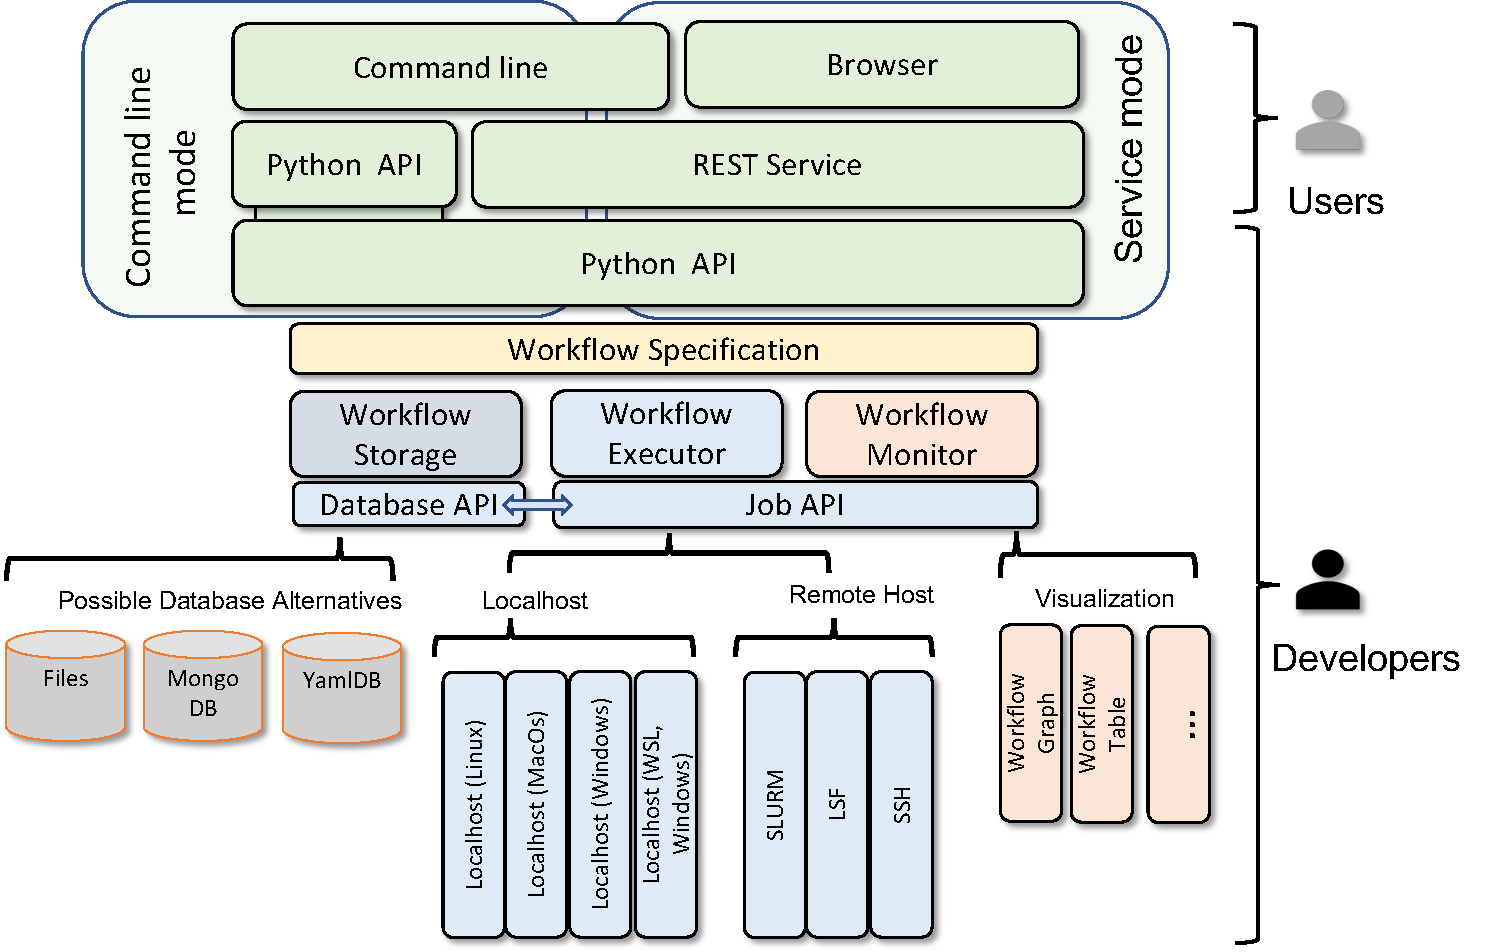
\includegraphics[width=1.0\columnwidth]{images/cloudmesh-cc-arch.pdf}
\caption{Architecture of the Cloudmesh-cc Framework.}\label{fig:arch}
\end{figure}

The framework is based on a layered architecture so it can be improved
and expanded on at each layer. We distinguish two kinds of users,
developers and endusers that define their own workflows to run on
compute resources. For the end user we provide a commandline and a
very simple browser interface. The simplicity is important as it does
not require to spend exorbitant amounts of time to learn how to use
the workflow framework. To support developers we have designed a
minimal Python API that is also used to implement a REST Service.
Currently the REST service is supposed to run on the client, but a
service deployment could also be conducted while assuring that proper
authentication and authorization is used. This is easily possible as
we use a well-known REST service framework (FastAPI) that can integrate
with common security frameworks to secure services. The API, workflow
specification, commandline interface, and browser are well documented
with the help of Sphinx and OpenAPI.

The workflow specification plays an important role to not only define
a workflow, but also to keep the status of a currently executed
workflow. Here we have completely separated the status of the workflow
and synchronize the state of the Workflow with pull requests to the
service that executes the computation. This allows the system to be
shut down at any time while the running jobs are completely
independent from the client application accessing the state. Thus the
client appears to be stateless and fetches the state of the submitted
jobs on demand. It will return the latest state found on the job
execution services.

The workflows are defined with YAML. The workflow is stored in a
database that can be implemented using a variety of backends such as
YamlDB which is file based, MongoDB, or pickle. In our current
implementation we just use a file-based implementation as it does not
require to set up and manage more complex databases. This is an
important capability as we found that scientists and beginning
students do not want to engage in the hassle of setting up and
managing a datastore such as MongoDB.

As we use a YAML file to represent the status of the workflow it is
easy to create monitoring components for example as part of a Web
browser. Various graph sophisticated display frameworks could be
used. For now we have simply exposed the graph in table format using
datatables.net and the graph as SVG while leveraging Graphviz.

One of the most important parts of the framework is how we manage jobs
and monitor their status. For this, we have introduced a abstract job
class that is integrated in our workflow class. The job class has the
ability to define jobs, start them, and cancel them, to name only the
most important management methods. However, each job defines a status
file in which the actual progress of the job is recorded. This status
file is managed on the compute resource where the job is run and is
queried on demand to return the status to the client. This way, the
status of all jobs can be monitored. As our goal is not to run jobs
that execute in milliseconds, but rather than in the second range such
status reporting and propagation is well suited for us. We have
defined a special status progress update specification that is
universally applicable. These jobs can be bash scripts, Python scripts,
Jupyter notebooks, or Slurm scripts.

Workflows are compilations of jobs to be run on nodes. These workflows
report information on the status of jobs as they are run, whether
locally or remotely.  These types of jobs can be mixed
with one another in a single workflow. This allows us, as already mentioned, 
to view the progress of a workflow as it is being run in quasi-realtime.
The workflow can be monitored as a graph or a datatable. These interfaces
report the statuses of the jobs. Additionally, the order in which the jobs
are run can be specified, enabling prerequisite jobs and the segmentation of a
workflow.

To address the requirement of simplicity the overall code is less than
3600 lines of code with additional 2600 lines for extensive test
cases.

The framework is managed as OpenSource repository in GitHub and uses
Python as the implementation language. The code is compatible with
Windows, macOS, and Linux.


\FILE{cc-design.tex}

\section{Design}

To fulfill our requirements, we have developed a framework for
workflow-controlled computing called Cloudmesh compute cluster,
otherwise referred to as {\em Cloudmesh-cc}. The architecture of the
framework is depicted in Figure~\ref{fig:arch}.

\begin{figure}[htb] \centering
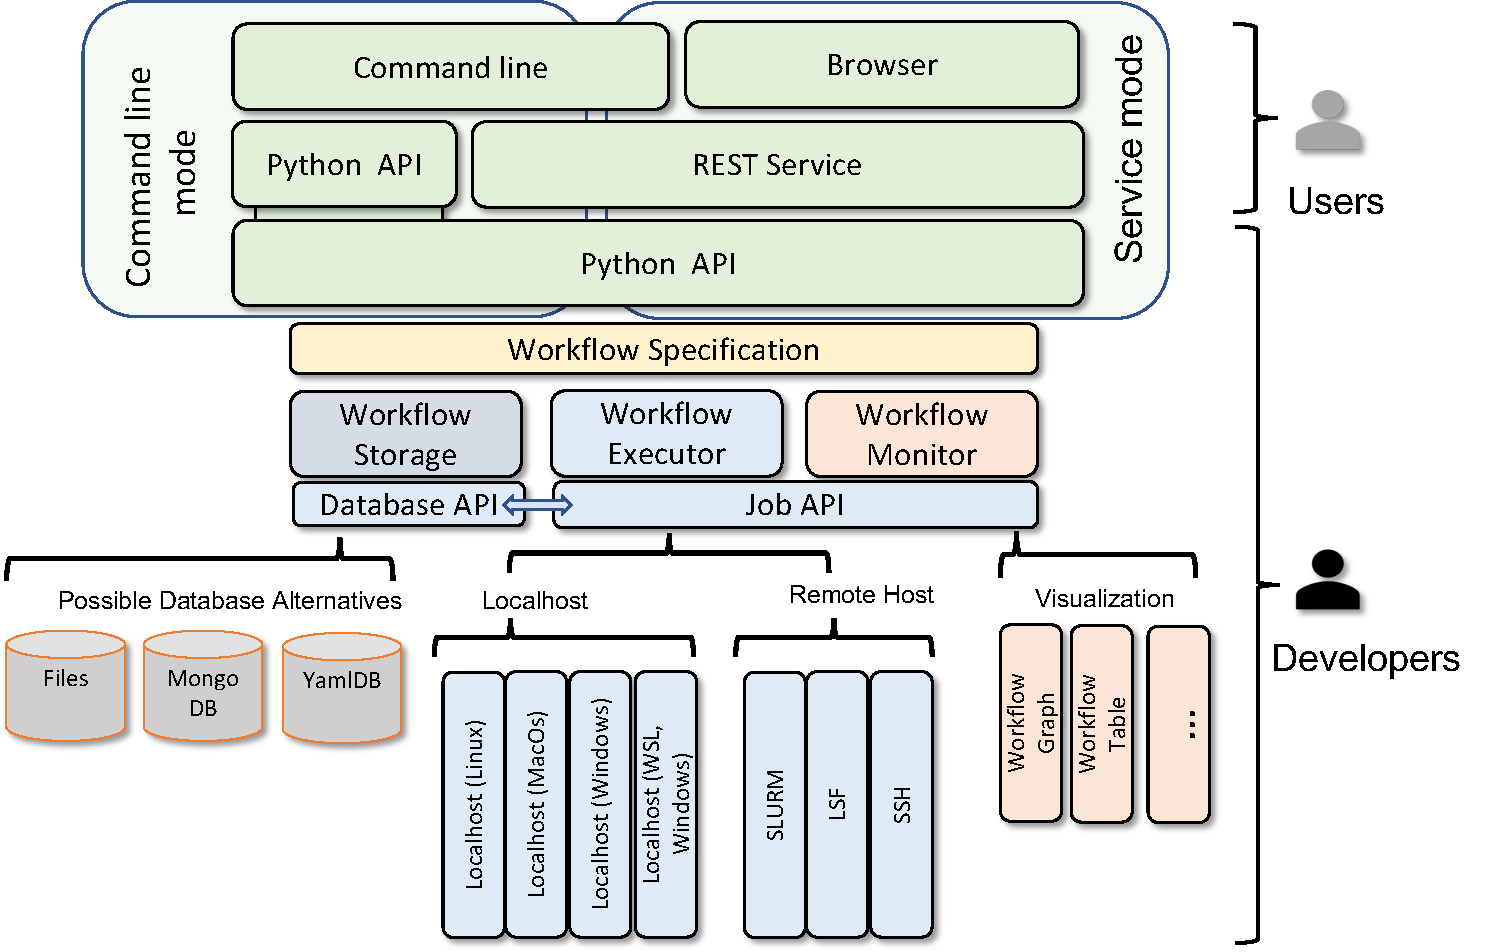
\includegraphics[width=1.0\columnwidth]{images/cloudmesh-cc-arch.pdf}
\caption{Architecture of the Cloudmesh-cc Framework}\label{fig:arch}
\end{figure}

The framework is based on a layered architecture so it can be improved
and expanded on at each layer. We distinguish two kinds of users,
developers and end users, that define their workflows to run on
compute resources. For the end user, we provide a command line and a
very simple browser interface. Simplicity is important as it does not
require spending exorbitant amounts of time to learn how to use the
workflow framework. To support developers, we have designed a minimal
Python API that is also used to implement a REST Service.  Currently,
the REST Service is supposed to run on the client, but a service
deployment could also be conducted while assuring that proper
authentication and authorization are used. This is easily possible as
we use a well-known REST service framework (FastAPI) that can
integrate with common security frameworks to secure services. The API,
workflow specification, command line interface, and browser are well
documented with the help of Sphinx and OpenAPI.

The workflow specification plays an important role in not only
defining a workflow but also keeping the status of a currently
executed workflow. Here we have completely separated the status of the
workflow and synchronize the state of the workflow with pull requests
to the service that executes the computation. This allows the system
to be shut down at any time while the running jobs are completely
independent of the client application accessing the state. Thus, the
client appears to be stateless and fetches the state of the submitted
jobs on demand. It will return the latest state found on the job
execution services.

The workflows are defined with YAML. The workflow is stored in a
database that can be implemented using a variety of backends such as
YamlDB (which is file-based), MongoDB, or pickle. In our current
implementation, we simply use a file-based implementation as it is not
required to set up and manage more complex databases. This is an
important capability as we found that scientists and beginning
students do not want to engage in the hassle of setting up and
managing a datastore such as MongoDB.

As we use a YAML file to represent the status of the workflow, it is
easy to create monitoring components (for example, as part of a Web
browser). Various sophisticated graph display frameworks could be
used. For now, we have simply exposed the graph in table format using
datatables.net and the graph as SVG while leveraging Graphviz.

One of the most important parts of the framework is how we manage jobs
and monitor their status. For this, we have introduced an abstract job
class that is integrated into our workflow class. The job class can
define jobs, start them, and cancel them, to name only the most
important management methods. However, each job defines a status file
in which the actual progress of the job is recorded. This status file
is managed on the compute resource where the job is run and is queried
on demand to return the status to the client. This way, the status of
all jobs can be monitored. As our goal is not to run jobs that execute
in milliseconds, but rather in the second range, such status reporting
and propagation is well-suited for us. We have defined a special
status progress update specification that is universally
applicable. These jobs can be bash scripts, Python scripts, Jupyter
notebooks, or Slurm scripts.

Workflows are compilations of jobs to be run on nodes. These workflows
report information on the status of jobs as they are run, whether
locally or remotely. These types of jobs can be mixed with others into
a single workflow. This allows us, as already mentioned, to view the
progress of a workflow as it is being run in quasi-realtime.  The
workflow can be monitored as a graph or a DataTable. These interfaces
report the statuses of the jobs. Additionally, the order in which the
jobs are run can be specified, enabling prerequisite jobs and the
segmentation of a workflow.

To address the requirement of simplicity, the overall code is less
than 3600 lines of code, with additional 2600 lines for extensive test
cases.

The framework is managed as an open-source repository in GitHub and
uses Python as the implementation language. The code is compatible
with Windows, macOS, and Linux.

% \section{Specifying Workflows}\label{specifying-workflows}

Users of cloudmesh cc must follow a certain configuration style to best
specify how a workflow should be run. Customization options include
specifying the job types, the order of how the jobs should be run, and
the portrayal of the graph.

\subsection{Workflow YAML format}\label{workflow-yaml-format}

A workflow yaml file with three Shell script jobs \texttt{a},
\texttt{b}, and \texttt{c} is as follows:

\begin{verbatim}
```text
workflow:
  nodes:
    a:
       name: a
       user: gregor
       host: localhost
       kind: local
       status: ready
       label: '{name}\nprogress={progress}'
       script: test-a.sh
    b:
       name: b
       user: gregor
       host: localhost
       kind: local
       status: ready
       label: '{name}\nprogress={progress}'
       script: test-b.sh
    c:
      name: c
      user: gregor
      host: localhost
      kind: local
      status: ready
      label: '{name}\nprogress={progress}'
      script: test-c.sh
  dependencies:
    - a,b,c
```
\end{verbatim}

\subsection{Example Workflows}\label{example-workflows}

Sample yaml files can be found at the following link:

\url{https://github.com/cloudmesh/cloudmesh-cc/blob/main/tests/workflow-example/workflow-example.yaml}

\subsection{Defining nodes in the
workflow}\label{defining-nodes-in-the-workflow}

Nodes can be customized in various ways within the workflow
configuration YAML file, including their job types (python, sh, jupyter,
or slurm), their virtual Python environment (by specifying
\texttt{venv}), their appearance on the graph, and other
characteristics.

\subsubsection{Defining labels for the
workflow}\label{defining-labels-for-the-workflow}

These variables must be in curly braces when defining the labels inside
the yaml workflow files.

For example, a label could be defined as follows:

\begin{verbatim}
```text
workflow:
  nodes:
    start:
      label: 'start\nCreated={created.%Y/%m/%d, %H--%M--%S}\nWorkflow Started={t0.%Y/%m/%d, %H--%M--%S}\nNow={now.%Y/%m/%d, %H--%M--%S}\nElapsed={dt0.%M--%S}'
```
\end{verbatim}

This creates a node on the graph that looks similar to the following
example:

\begin{figure}
\centering
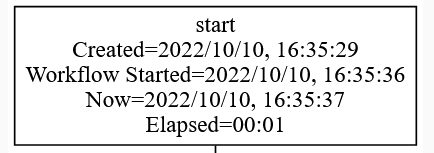
\includegraphics{images/labelmaker-example.png}
\caption{An example node with labels}
\end{figure}

Initially, the created and elapsed labels are \texttt{N/A} if the
workflow has not yet started, but they are replaced during runtime. This
can be observed by running a workflow in graph view in the web
interface.

Colons must be replaced with \texttt{-\/-} and the years, months, days,
hours, minutes, and seconds can be arranged as desired, as long as the
corresponding letters remain consistent (\texttt{\%Y} \texttt{\%m}
\texttt{\%d} \texttt{\%H} \texttt{\%M} \texttt{\%S} respectively). Also,
the format of the time must come immediately following the period.

\begin{itemize}
\tightlist
\item
  \texttt{name} name of job
\item
  \texttt{progress} progress of job from 0-100
\item
  time labels:

  \begin{itemize}
  \tightlist
  \item
    \texttt{now.} current time
  \item
    \texttt{now.\%Y/\%m/\%d,\ \%H-\/-\%M-\/-\%S} now in particular
    format (this can be used for other times as well)
  \item
    \texttt{created.} time when workflow was created
  \item
    \texttt{t0.} workflow start time
  \item
    \texttt{t1.} workflow end time
  \item
    \texttt{dt0.} elapsed time since workflow began
  \item
    \texttt{dt1.} total time of workflow once complete
  \item
    \texttt{tstart.} job start time
  \item
    \texttt{tend.} job end time
  \item
    \texttt{modified.} job modified time
  \end{itemize}
\item
  \texttt{os.} operating system environment variable (like os.HOME)
\item
  \texttt{cm.} cloudmesh variable that is read from \texttt{cms\ set}
\end{itemize}

\subsection{Defining format for timestamp
labels}\label{defining-format-for-timestamp-labels}

Various formats can be used for the timestamps, such as the American
datetime format \texttt{\%m/\%d/\%Y,\ \%H-\/-\%M-\/-\%S} or the
international datetime format \texttt{\%Y/\%m/\%d,\ \%H-\/-\%M-\/-\%S}.
As long as the letters stay consistent (\texttt{\%Y} \texttt{\%m}
\texttt{\%d} \texttt{\%H} \texttt{\%M} \texttt{\%S} for year, month,
day, hour, minute, and second, respectively), any format can be created.

If no format is specified following the period after the variable, the
datetime defaults to American format.

\subsection{Defining graphviz shapes and
styles}\label{defining-graphviz-shapes-and-styles}

Any shape and style for the nodes in the graph can be chosen, as long as
they are taken from the graphviz documentation:

\url{https://graphviz.org/doc/info/shapes.html}

\url{https://graphviz.org/docs/attr-types/style/}

The following is an example of a node in YAML format that uses a box
shape and an empty style. The empty style defaults to \texttt{filled},
which allows the node to change color when the job status is changed.

\begin{verbatim}
```text
workflow:
  nodes:
    start:
      label: 'start\nCreated={created.%Y/%m/%d, %H--%M--%S}\nWorkflow Started={t0.}\nElapsed={dt0.}'
      kind: local
      user: grey
      host: local
      status: ready
      exec: 'echo hello'
      name: start
      shape: box
      style: ''
```
\end{verbatim}

\subsection{Defining dependencies in the
workflow}\label{defining-dependencies-in-the-workflow}

Dependencies are specified in the order which jobs should be run, from
left to right. They are listed under the workflow in the yaml file.

\begin{verbatim}
```bash
workflow:
  nodes:
    a:
       name: a
    b:
       name: b
    c:
       name: c
  dependencies:
    - a,b,c
```
\end{verbatim}

\subsection{Reporting Progress}\label{reporting-progress}

When running scripts/jobs inside a workflow, the scripts must leverage
some format of cloudmesh.progress to run successfully. Otherwise, the
Workflow class cannot tell if the scripts are done, breaking the
progress functionality.

The examples that are provided with cloudmesh-cc are already augmented
with cloudmesh.progress. Thus, if a user is running self-made jobs and
workflows, they must adhere to the guidelines as follows.

\subsection{Shell and Slurm Scripts}\label{shell-and-slurm-scripts}

For shell and Slurm scripts \texttt{.sh}, the script must contain:

\begin{verbatim}
```bash
echo "# cloudmesh status=running progress=1 pid=$$"
```
\end{verbatim}

at the beginning of the script, and

\begin{verbatim}
```bash
echo "# cloudmesh status=done progress=100 pid=$$"
```
\end{verbatim}

at the end of the script.

\subsection{Python Scripts and Jupyter
Notebooks}\label{python-scripts-and-jupyter-notebooks}

For Python scripts \texttt{.py} and Jupyter notebooks \texttt{.ipynb},
the script must contain an import module from cloudmesh.common and calls
to the progress function.

py\_script.py

\begin{verbatim}
```bash
from cloudmesh.common.StopWatch import progress
from cloudmesh.common.Shell import Shell
filename = Shell.map_filename('./py_script.log').path
progress(progress=1, filename=filename)

# your script does what you want it to do here...

progress(progress=100, filename=filename)
```
\end{verbatim}

The statements do not need to be at the absolute beginning or end of the
script, but the progress must:

\begin{itemize}
\tightlist
\item
  be written to a filename with the same name as the script, ending in
  \texttt{.log}
\item
  begin at progress=1
\item
  and end at progress=100
\end{itemize}



\FILE{specifying-workflows.tex}

\section{Specifying Workflows}\label{specifying-workflows}

The workflow definition for cloudmesh is rather simple and intuitive.
An example is provided in Figure~\ref{fig:workflow-example}. Here, a
DAG with three nodes are specified ($start \rightarrow fetch-data
\rightarrow compute \rightarrow analyze \rightarrow end$). The
workflow executes three scripts
(test-[fetch-data,compute,analyze].sh). It contains a specific start
and end node.

\subsection{Dependencies}

Each dependency is specified in the {\em dependency} section while
providing sequences of names in a list such as \mintinline{bash}|-
start,fetch-data| or, in our case where 3 more nodes are defined,
additional nodes are appended with commas, as in
\mintinline{bash}|,compute,analyze,end|.

In case one wants to execute nodes in parallel, we can simply define
them through a list such as 

\begin{minted}[breaklines]{yaml}
  dependencies:
    - start,a,end
    - start,b,end
    - start,c,end
\end{minted}

if the names of the nodes were $a$, $b$, and $c$. 


\subsection{Nodes}

Nodes can be customized in various ways within the workflow
configuration YAML file, including their job types (python, sh,
jupyter, or slurm), their virtual Python environment (by specifying
\mintinline{bash}|venv|), their appearance on the graph, and other
characteristics. This is controlled through a number of attributes
used by the nodes in the DAG. The attributes are summarized in
Table~\ref{tab:node-attributes}.

\begin{figure}
\begin{minted}[breaklines]{yaml}
workflow:
  nodes:
    start:
       name: start
    fetch-data:
       name: fetch-data
       user: gregor
       host: localhost
       kind: local
       status: ready
       label: '{name}\nprogress={progress}'
       script: test-fetch-data.sh
    compute:
       name: compute
       user: gregor
       host: localhost
       kind: local
       status: ready
       label: '{name}\nprogress={progress}'
       script: test-compute.sh
    analyze:
      name: analyze
      user: gregor
      host: localhost
      kind: local
      status: ready
      label: '{name}\nprogress={progress}'
      script: test-analyze.sh
    end:
       name: end
  dependencies:
    - start,fetch-data,compute,analyze,end
\end{minted}
\caption{Workflow YAML Configuration file.}\label{fig:workflow-example}
\label{fig:yaml-file}
\end{figure}

\begin{table}[htb]
\caption{Node attributes.}\label{tab:node-attributes}
\resizebox{1.0\columnwidth}{!}{
\begin{tabular}{|l|p{6cm}|}
\hline
{\bf Attribute} & {\bf Description} \\
\hline
\hline
name &  A unique name of the job, must be the same as defined in the : line \\
\hline
user &  The username for the host \\
\hline
host &  The hostname \\
\hline
kind &  The kind of the job, which can be local, ssh, wsl, or slurm  \\
\hline
status &  The status of the job in integer value between 0 and 100 \\
\hline
label &  A custom designed label \\
\hline
script &  The script name to be executed \\
\hline
\end{tabular}
}
\end{table}

\subsection{Node labels}

One particular useful attribute is that of a label. If no label is
used, the name of the node is used as the label. However, if a label
is specified, one can also use attribute names and timers to create
labels with implicit state information. This is done by introducing
variables through curly braces when defining the labels inside the
label defined in nodes within the YAML workflow file.

For example, a label could be defined as showcased in
Figure~\ref{fig:label-job}. The appropriate values will be dynamically
replaced during the execution of the workflow.  This creates a node on
the graph that looks similar to the node showcased in
Figure~\ref{fig:label-node}.

Initially, the created and elapsed labels are \mintinline{bash}|N/A|
if the workflow has not yet started, but they are replaced during
runtime. This can be observed by running a workflow in graph view in
the web interface.

In this format, we must use two dashes \mintinline{bash}|--| to
separate the various components.  However, when rendered, the dashes
will be replaced with a colon.  Thus you can easily use years, months,
days, hours, minutes, and seconds can be arranged as desired, as long
as the corresponding letters remain consistent:
(\mintinline{bash}|%Y| 
\mintinline{bash}|%m|
\mintinline{bash}|%d| 
\mintinline{bash}|%H| 
\mintinline{bash}|%M| 
\mintinline{bash}|%S|).
The time format must be specified immediately following the period
after a format-supported time variable.  If no format is specified
following the period after the variable, the datetime defaults to the
American format.  See Table~\ref{fig:labels-list} for a summary of
options for defining time based attributed to being replaced in the
label.


Nodes can be customized in various ways within the workflow
configuration YAML file, including their job types (python, sh,
jupyter, or slurm), their virtual Python environment (by specifying
\mintinline{bash}|venv|), their appearance on the graph, and other
characteristics.


\begin{figure}
\smallskip
    \begin{minted}[breaklines]{yaml}
    workflow:
      nodes:
        start:
          label: 'start\nCreated={created.%Y/%m/%d, %H--%M--%S}\nWorkflow Started={t0.%Y/%m/%d, %H--%M--%S}\nNow={now.%Y/%m/%d, %H--%M--%S}\nElapsed={dt0.%M--%S}'
    \end{minted}
    \caption{Example of job label in YAML configuration file.}
    \label{fig:label-job}

\centering
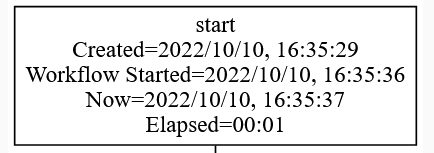
\includegraphics[width=0.7\columnwidth]{images/labelmaker-example.png}
\caption{An example node with labels.}\label{fig:label-node}
\end{figure}

\begin{table}[htb]
\caption{List of possible labels for nodes on the graph.}
\label{fig:labels-list}

{\footnotesize
  \begin{tabular}{|p{3.5cm}|p{4cm}|}
    \hline
    {\bf Name} & {\bf Description} \\
    \hline
    \hline
    progress &  progress of job from 0-100 \\
    \hline
    now & current time \\
    \hline
    now.\verb|%Y%m%d,%H--%M--%S| &
   now in particular format (this can be used for other times as well) \\
    \hline
    created & time when workflow was created \\
    \hline
    t0.\verb|%Y%m%d,%H--%M--%S| &  workflow start time \\
    \hline
    t1.\verb|%Y%m%d,%H--%M--%S| & workflow end time \\
    \hline
    dt0.\verb|%Y%m%d,%H--%M--%S| & elapsed time since workflow began \\
    \hline
    dt1.\verb|%Y%m%d,%H--%M--%S| & total time of workflow once complete \\
    \hline
    tstart.\verb|%Y%m%d,%H--%M--%S| & job start time \\
    \hline
    tend.\verb|%Y%m%d,%H--%M--%S| & job end time \\
    \hline
    modified.\verb|%Y%m%d,%H--%M--%S| & job modified time \\
    \hline
    os. & operating system environment variable (like os.HOME) \\
    \hline
    cm. & cloudmesh variable that is read from \verb|cms set| \\
    \hline
\end{tabular}
}
\end{table}



\subsection{Shapes and Styles}

As we use graphviz for rendering, we have also added the ability to
change the shape and style of each node in the graph. The
available \href{https://graphviz.org/doc/info/shapes.html}{shapes}
and \href{https://graphviz.org/docs/attr-types/style/}{styles} are
listed in the Graphviz documentation \cite{www-graphviz}.

Figure~\ref{fig:shape-style-yaml} is an example of a node in YAML
format that uses a box shape and an empty style. The empty style
defaults to \mintinline{bash}|filled|, which allows the node to change
color when the job status is changed.

\begin{figure}
    \begin{minted}[breaklines]{yaml}
    workflow:
      nodes:
        start:
          label: 'start\nCreated={created.%Y/%m/%d, %H--%M--%S}\nWorkflow Started={t0.}\nElapsed={dt0.}'
          kind: local
          user: grey
          host: local
          status: ready
          exec: 'echo hello'
          name: start
          shape: box
          style: ''
    \end{minted}
    \caption{Example of YAML config file that uses shape and style.}
    \label{fig:shape-style-yaml}
\end{figure}



\subsection{Reporting Progress}\label{reporting-progress}

When running scripts/jobs inside a workflow, the scripts must leverage
some format of {\em cloudmesh.progress} to notify the user and the
backend client monitoring system. If progress is not reported, the
Workflow class cannot tell if the scripts are done.

The examples that are provided with cloudmesh-cc are already augmented
with {\em cloudmesh.progress}. Thus, if a user is running jobs through
cloudmesh cc workflows, they must integrate progress strings into the
log files that are monitored. This is available for shell, batch,
Python, and Jupyter scripts.

For shell and Slurm scripts, the script must contain a progress update
lines as follows:

\begin{minted}[breaklines]{bash}
echo "# cloudmesh status=running progress=1 pid=$$"
\end{minted}

at the beginning of the script, and

\begin{minted}[breaklines]{bash}
echo "# cloudmesh status=done progress=100 pid=$$"
\end{minted}

at the end of the script.

For Python scripts and Jupyter notebooks, it is easiest to use our
built-in progress method and import it from the cloudmesh.common
module. The following example demonstrates its use:

\smallskip
\begin{minted}[breaklines]{python}
from cloudmesh.common.StopWatch import progress
from cloudmesh.common.Shell import Shell
filename = Shell.map_filename('./py_script.log').path
progress(progress=1, filename=filename)
# execute your analysis here ...
progress(progress=100, filename=filename)
\end{minted}
\smallskip

When recording progress, the progress should be ascending between 1
and 100. The last value must report 100 or the node will not be
completed and the workflow gets stuck. The output of the progress will
be written into a {\scriptsize \verb|{workflowname}.log|} file that
will be probed continuously by the client to report the progress to
the user.

\subsection{Generating Progress Image as Graph}

The framework has a built-in capability to export the progress of the
workflow in a DAG.

In Figure~\ref{fig:workflow-process}, we depict a simple example
workflow to be executed, where each task is executed sequentially. The
status of the execution can be displayed as a table or as a graph. In
Figure~\ref{fig:workflow-process}, we showcase how the graph changes
its appearance over time while using no label in the start and end
node and a defined label in the nodes for fetch-data, compute, and
analyze:

\begin{minted}[breaklines]{bash}
label: "{name}\nprogress={progress}"
\end{minted}

\begin{figure}[htb]
\resizebox{1.0\columnwidth}{!}{
\begin{minipage}[b]{0.18\textwidth}
Definition and start \\
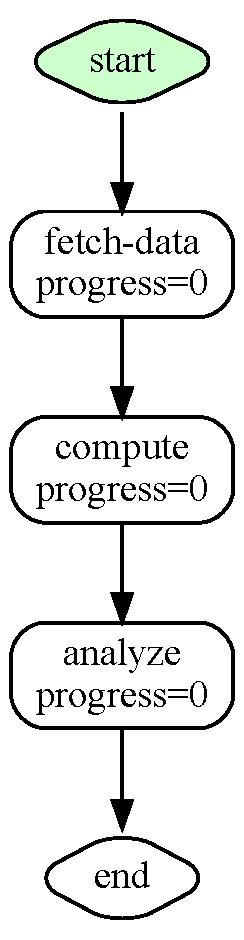
\includegraphics[height=9cm]{images/workflow-example-1.pdf}
\end{minipage} \ \
\begin{minipage}[b]{0.18\textwidth}
Running 1st task \\
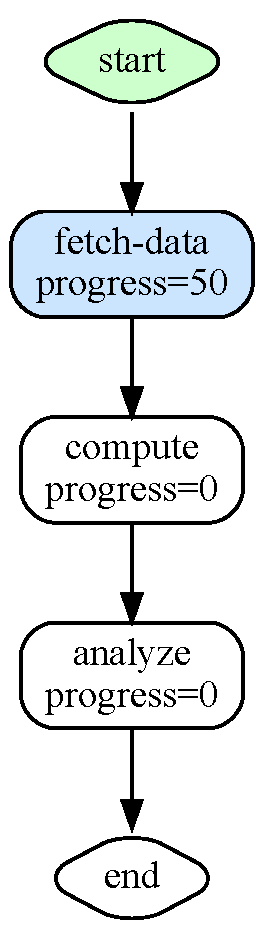
\includegraphics[height=9cm]{images/workflow-example-1.5.pdf} 
\end{minipage} \ \
\begin{minipage}[b]{0.18\textwidth}
Complete 1st task \\
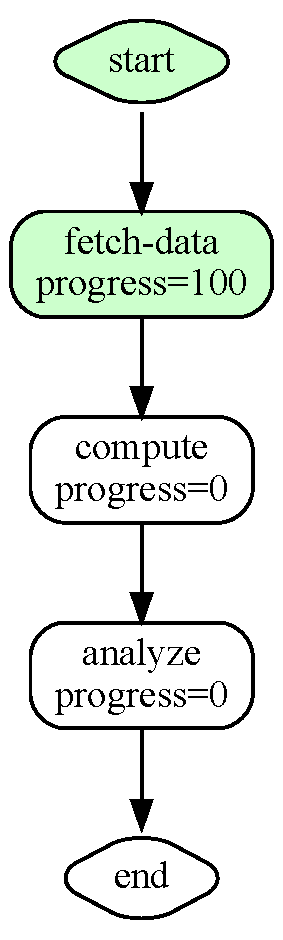
\includegraphics[height=9cm]{images/workflow-example-2.pdf}
\end{minipage} \ \
\begin{minipage}[b]{0.18\textwidth}
Complete 2nd task \\
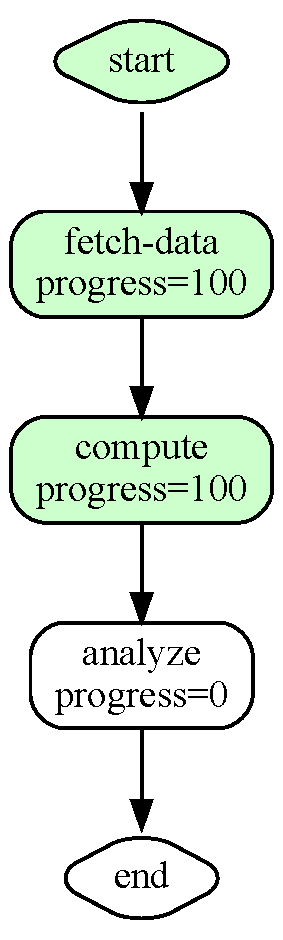
\includegraphics[height=9cm]{images/workflow-example-3.pdf}
\end{minipage} \ \
\begin{minipage}[b]{0.18\textwidth}
Complete workflow \\
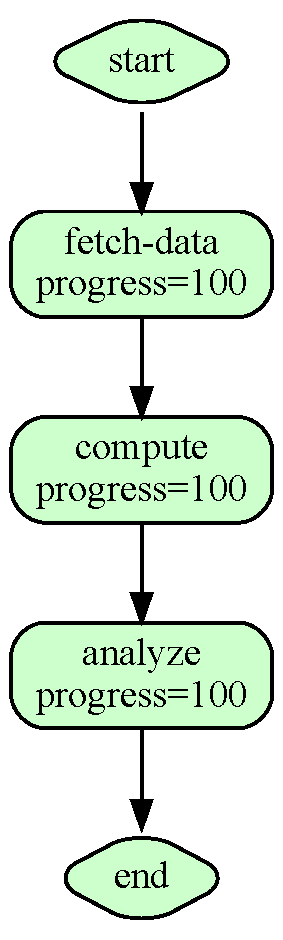
\includegraphics[height=9cm]{images/workflow-example-5.pdf}
\end{minipage} 
}
\caption{The gradual process of a simple workflow.}\label{fig:workflow-process}
\end{figure}





% \FILE{quickstart.tex}

\section{Cloudmesh-cc Interfaces}

In this section we explain the various ways of interfacing with cloudmesh-cc.

It is important to note that we have a {\em commandline mode} that interfaces directly with the backends while not requiering a service. This includes an easy to use python API.

In addition we have used this API to implement a {\em service mode}, so we an stand up a REST service as well as a GUI that can ba accessed through a Web browser.
Please note that the service mode can also be access through te command line in a terminal. To distinguish how we operate cloudmesh-cc we use the term {\em mode} to deliniate it from a command that is entered ina terminal to query the status of the workflow.

We will now discuss tes interfaces in more detail and also showcase
hwo we can access them.


\subsection{Python API}

Cloudmesh-cc is implemented in Python. Extensive documentation is
available in GitHub and through GitHub action it is automatically
updated \cite{github-cloudmesh-cc}.  We distingush two main classes
that are easy to use. The first is a {\em Job class} that can adapted
to include new computational resource types for executing jobs. The
second is a {\em Workflow class} to ccordinate the execution of
multiple jobs. Selected methods of the Job class include are listed in
Figure~\ref{fig:code-job}. Important to note is that the code for the
scripts are all managed locally and a synchronization step is invoked
prior to one running the job to assure that the latest script and
code to be executed on the compute resource is available.

The most important part of using the Workflow Python API is showcased
in Figure~\ref{fig:code-job}, where we explain how easy it is to set up a workflow
with the Python API.

\begin{figure}[!h]
\begin{minted}[breaklines]{bash}
class Job:
   ...
   def clear():
      """Clear job progress."""
   def create(filename=None, script=None, exec=None):
      """Create a template for the script with progress."""
   def get_log(refresh=True):
      """Get the log of the job."""
   def get_pid(refresh=False):
      """Get the pid that the job is running within determined by the compute resource it is running on."""
   def get_progress(refresh=False):
       """Get the progress of the job from the compute resource."""
   def get_status(refresh=False):
       """Get the status of the job."""
   def kill():
       """Kill the job."""
   def run():
       """Run the job."""
   def sync():
       """Synchronise the current directory with the remote. Copies the shell script to the experiment directory and ensures that the file is copied with the sync command."""
   def watch(period=10):
       """Watch the job and check for changes in the given period."""
\end{minted}
\caption{Pseudo code for the Job class with selected methhods}
\label{fig:code-job}

\bigskip

\begin{minted}[breaklines]{bash}
class Workflow:
    ...
    def add_dependencies(dependency)
        """Add a job dependency to the workflow (and the graph)."""
    add_dependency(source, destination)
        """Add a job dependency to the workflow (and the graph)."""
    def add_job( ... ):
        """Add a job to the workflow with appropriate parameters."""
    def display(filename=None, name='workflow', first=True)
        """Show the graph of the workflow."""
    def job(name):
        """Return the details of a job within the workflow."""
    def load(filename, clear=True)
        """Load the workflow."""
    def remove_job(name, state=False)
        """Remove a particular job from the workflow."""
    def remove_workflow()
        """Delete workflow from the local file system."""
    def run_parallel( ... )
        """Run a workflow in a parallel fashion."""
    def run_topo(order=None, dryrun=False, show=True, filename=None)
        """Run the workflow in a topological order."""
    def save(filename=None):
        """Save the workflow."""
    def save_with_state(filename, stdout=False):
        """Save the workflow with state."""
    def sequential_order():
        """Return a list of the topological order of the workflow."""
    property table
        """Return a table of the workflow."""
    def update_progress(name):
        """Manually update the progress of a job according to its log file."""
    def update_status(name, status):
        """Manually update a job’s status."""
\end{minted}
\caption{Pseudo code for the Job class with selected methhods}
\label{fig:code-workflow}
\end{figure}


\begin{figure}[htb]
\begin{minted}[breaklines]{bash}
    w = Workflow(name="workflow-analyze")
    # load a preexisting workflow
    # w.load(filename="source.yaml")
    
    # add jobs and dependencies explicitly
    w.add_job(name="fetch-data",
              exec="hostname",
              host='supercomputer-a' # defined in .ssh
              label="{name}\nprogress={progress}",
              kind="local",
              status="ready",
              progress=0)
    w.add_job(name="compute", command="... TBD ...")
    w.add_job(name="analyze", command="... TBD ...")
    w.add_dependencies(
              dependency="start,fetch-data,compute,analyze")
    w.run_topo()
\end{minted}
\caption{Pseudo code for the Job class with selected methods}
\label{fig:code-workflow-example}

\bigskip

\begin{minted}[breaklines]{bash}
      cms cc workflow add [--name=NAME] [--job=JOB] ARGS...
      cms cc workflow add [--name=NAME] --filename=FILENAME
      cms cc workflow delete [--name=NAME] [--job=JOB]
      cms cc workflow list [--name=NAME] [--job=JOB]
      cms cc workflow run [--name=NAME] [--job=JOB] [--filename=FILENAME]
      cms cc workflow [--name=NAME] --dependencies=DEPENDENCIES
      cms cc workflow status --name=NAME [--output=OUTPUT]
      cms cc workflow graph --name=NAME
\end{minted}
\caption{Command line interface to the workflow in terminal mode}
\label{fig:code-workflow-commandline}

\bigskip

\begin{minted}[breaklines]{bash}
      cms cc start [-c] [--reload] [--host=HOST] [--port=PORT]
      cms cc stop
      cms cc status
      cms cc workflow service add [--name=NAME] FILENAME
      cms cc workflow service list [--name=NAME] [--job=JOB]
      cms cc workflow service add [--name=NAME] [--job=JOB] ARGS...
      cms cc workflow service run --name=NAME
\end{minted}
\caption{Command line interface to the workflow in service mode}
\label{fig:code-workflow-service-commandline}.

% \bigskip

{\centering
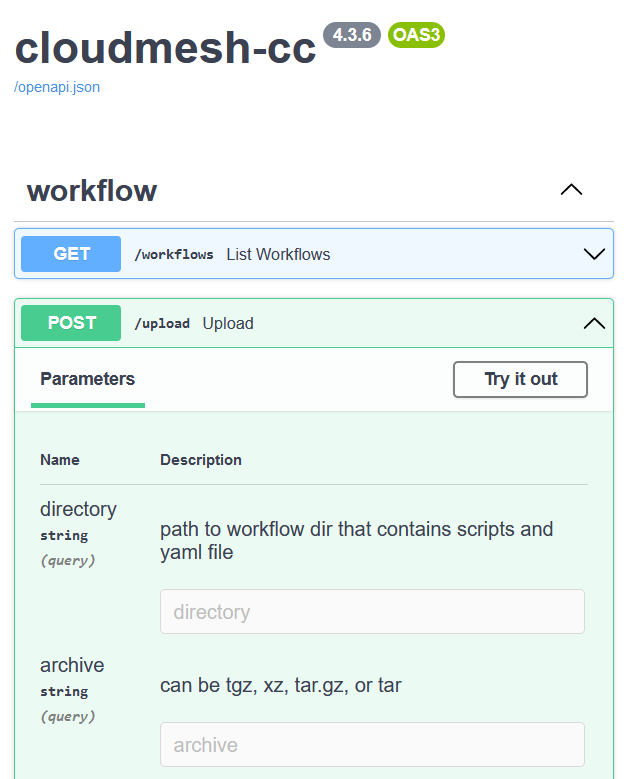
\includegraphics[width=0.52\columnwidth]{images/upload_api.png}
}
\caption{Browser API GUI for Cloudmesh Compute Cluster}

\label{fig:openapi}

\end{figure}


\subsection{Commandline Mode}

The commandline mode is an implementation that does not use a backend
service. It runs in the terminal until the workflow is completed. All
states of the jobs are managed on the compute service on which the job
is run and the status is replicated into the client on demand. This
allows easy reporting of the status through a table and a graph
display using client based rendering tools. The various commands to
interact with it on the commandline are shown in
Figure~\ref{fig:code-workflow-commandline}.


\subsection{Service Mode}

The Python API has ale been used to implement a REST service. To
easily interact with the REST service we have also added a couple of
conveneinet commannds one can issue from a terminal. They are listed
in Figure~\ref{fig:code-workflow-service-commandline}. It is clear for
these methods that starting stopping and getting the status of the
service is very easy, In contrast to the commandline mode this service
mode has an additional keyword {\em service} to interact with the rest service.

Certainly one can also directly interact with the REST service API for
this service. For ease of use we have exposed the interface through
an OpenAPI specification that is available to the user as shown in
Figure~\ref{fig:openapi}.



Thus other tools such as curl or other languages supporting url
requests can be used. A curl example to list the workflow
specifications uploaded to the service is

As we use a REST service, we can also easily upload the workflow
through a Python enabled REST call. We will use Python requests to
demonstrate this upload feature. To showcase the various ways to
access the service we focus on uploading a tar file that contains the workflow as well as the scripts or programs used in the workflow. The tar file is called {\em workflow.tar}

To also allow programming against the REST service in Python a Python
API similar to that pf the commandline mode is
available. Figure~\ref{fig:code-workflow-rest-commandline} showcases
this API.

To simplify interaction with the Rest service we create a special
RESTWorkflow class that is similar to the command module API but uses
instead the REST interface to the service rather than directly
communication with the command client API.

If the user wants to use instead just Python requests he can do so as
follows, while we just showcase the program in
Figure~\ref{fig:code-workflow-requests} for uploading.

\begin{figure}[t]
\begin{minted}[breaklines]{bash}
class RESTWorkflow
    ...
    def add_job(workflow_name, **kwargs):
        """Add a job to the workflow."""
    def delete_workflow(workflow_name, job_name=None):
        """Delete a workflow by using REST."""
    def get_workflow(workflow_name, job_name=None):
        """Retrieve a workflow by using REST."""
    def list_workflows():
        """Return a list of workflows that is found within
           the server."""
    def run_workflow( ... ):
        """Run a workflow by using REST."""
    def upload_workflow( ... ):
        """Upload a workflow by using REST."""
\end{minted}
\caption{Pseudo code for the Job class with selected methods}
\label{fig:code-workflow-rest-commandline}

\bigskip

\begin{minted}[breaklines]{python}
import requests
r = requests.post(
      'http://127.0.0.1:8000/workflow?archive=workflow-example.tar')
print(r.text)
\end{minted}
\caption{Upload to the REST service with Python requests}
\label{fig:code-workflow-requests}

\bigskip

\begin{minted}[breaklines]{bash}
$ curl -X 'POST' 'http://127.0.0.1:8000/ workflow?archive=workflow-example.tar'                           -H 'accept: application/json' -d ''
\end{minted}%$
\caption{Upload to the REST service with curl}
\label{fig:code-workflow-curl}

\end{figure}


\subsection{Webservice GUI}

A convenient Web service is included in Cloudmesh cc. It allows the user
to manage and visualize the status of workflows through a Web browser
interface. At this time the focus is that the interface can be run by a
singleuser on the local machine. This allows that remote executions of
workflow nodes run completely independent from cloudmesh cc and
interaction is possible in asynchronous mode.

As the service is using also an OpenAPI 2.0 specification the workflow
can also be uploaded implicitly through the specification
GUI. Navigate to \texttt{http://127.0.0.1:8000/docs} and use the POST
Upload method. Then click \texttt{Try\ it\ out} and enter the
location of the tar file, followed by clicking {\em Execute}.

Obviously, any REST service or REST API can be used allowing to
interface to it from different programming languages or frameworks.

The web server provides a more customizable, easy-to-use interface for
the Workflow class which can be started, viewed, and stoped with the
appropriate command line. 

\begin{minted}[breaklines]{bash}
  $ cms cc start
  $ cms cc view
  $ cms cc stop
\end{minted}%$

The view can also be achieved by opening the 
the link {\scriptsize \verb|http://127.0.0.1:8000/}.

Now the browser provides an interface to view preexisting workflows in both
a DataTable format and as a graph format. Both views will update
automatically, in a live fashion, as the workflows are run, reporting
live job status and progress.

For a quick and easy example of leveraging this GUI interface, click
on the Example tab in the left-hand sidebar. Then, a workflow-example
will appear underneath Workflows. Click on the workflow-example and
run the workflow by clicking the green Run button in the top-right. As
the workflow runs, the user is able to click on the Graph button (see
Figure~\ref{fig:graph}) and back to the Table button (see
Figure~\ref{fig:table}, as desired, to view the workflow's
progression.


\begin{figure}[htb]
{\centering
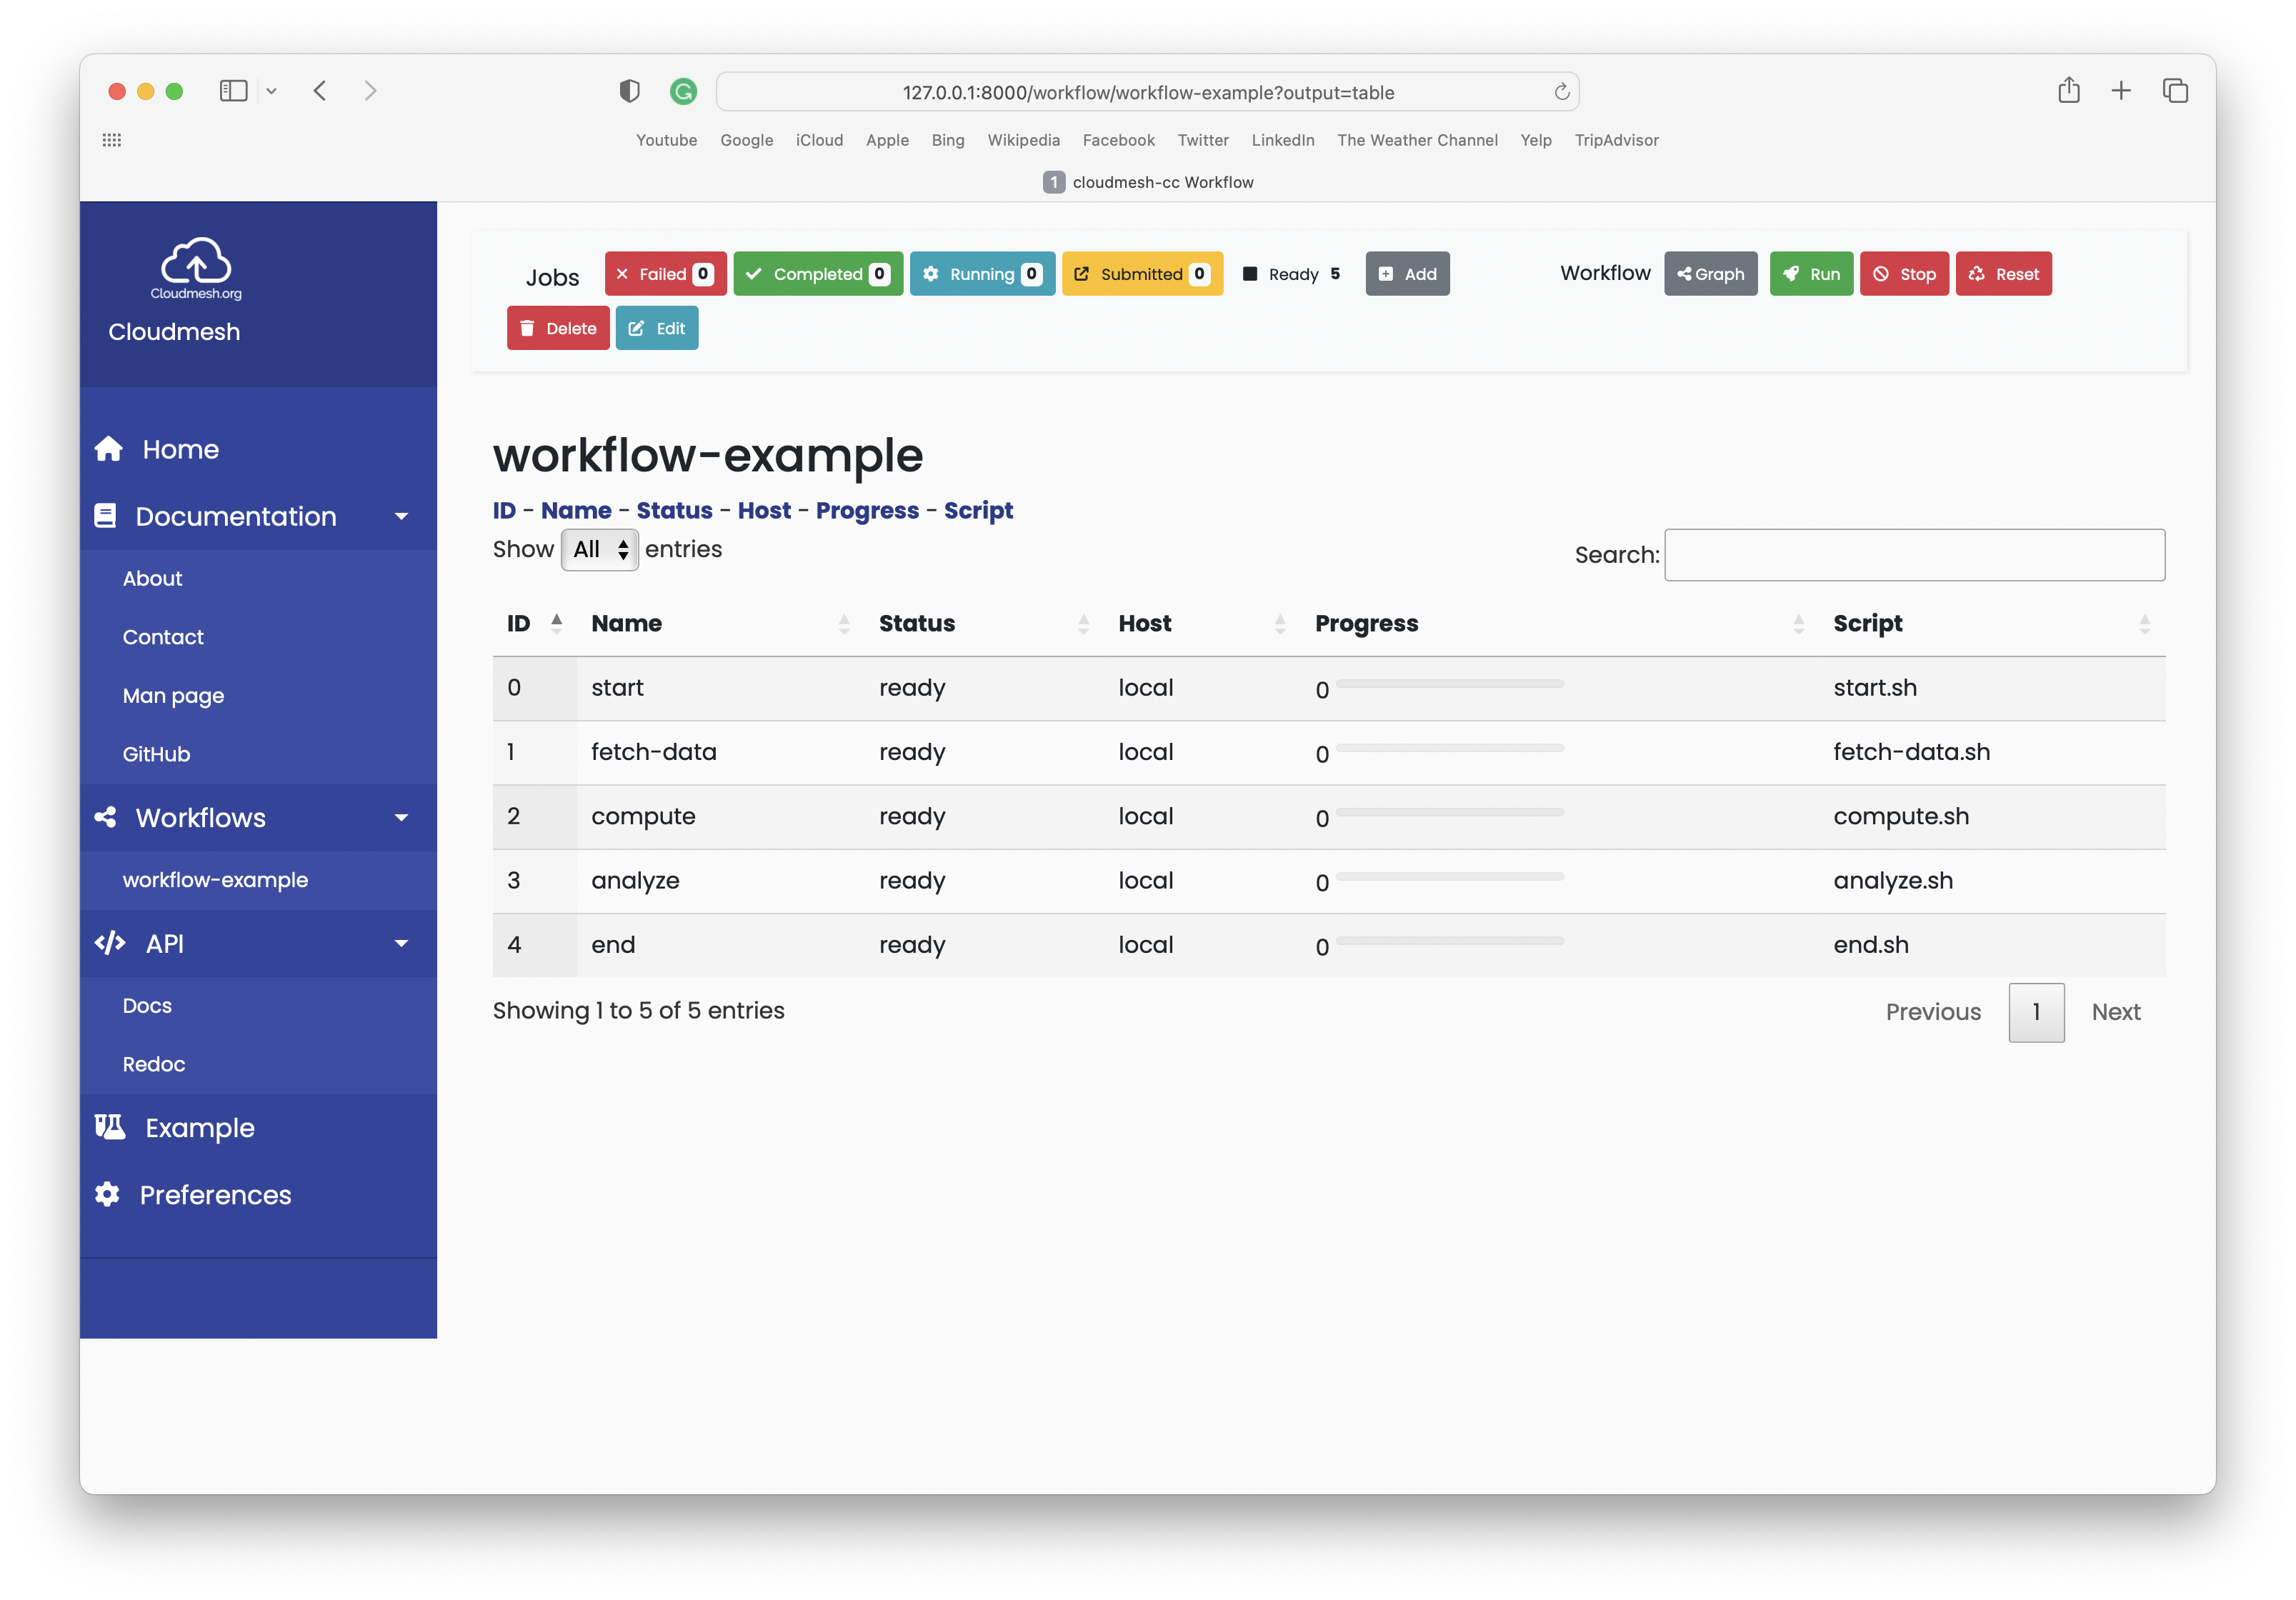
\includegraphics[width=1.05\columnwidth]{images/service-table.png}}
\caption{Cloudmesh cc workflow table view}\label{fig:table}

{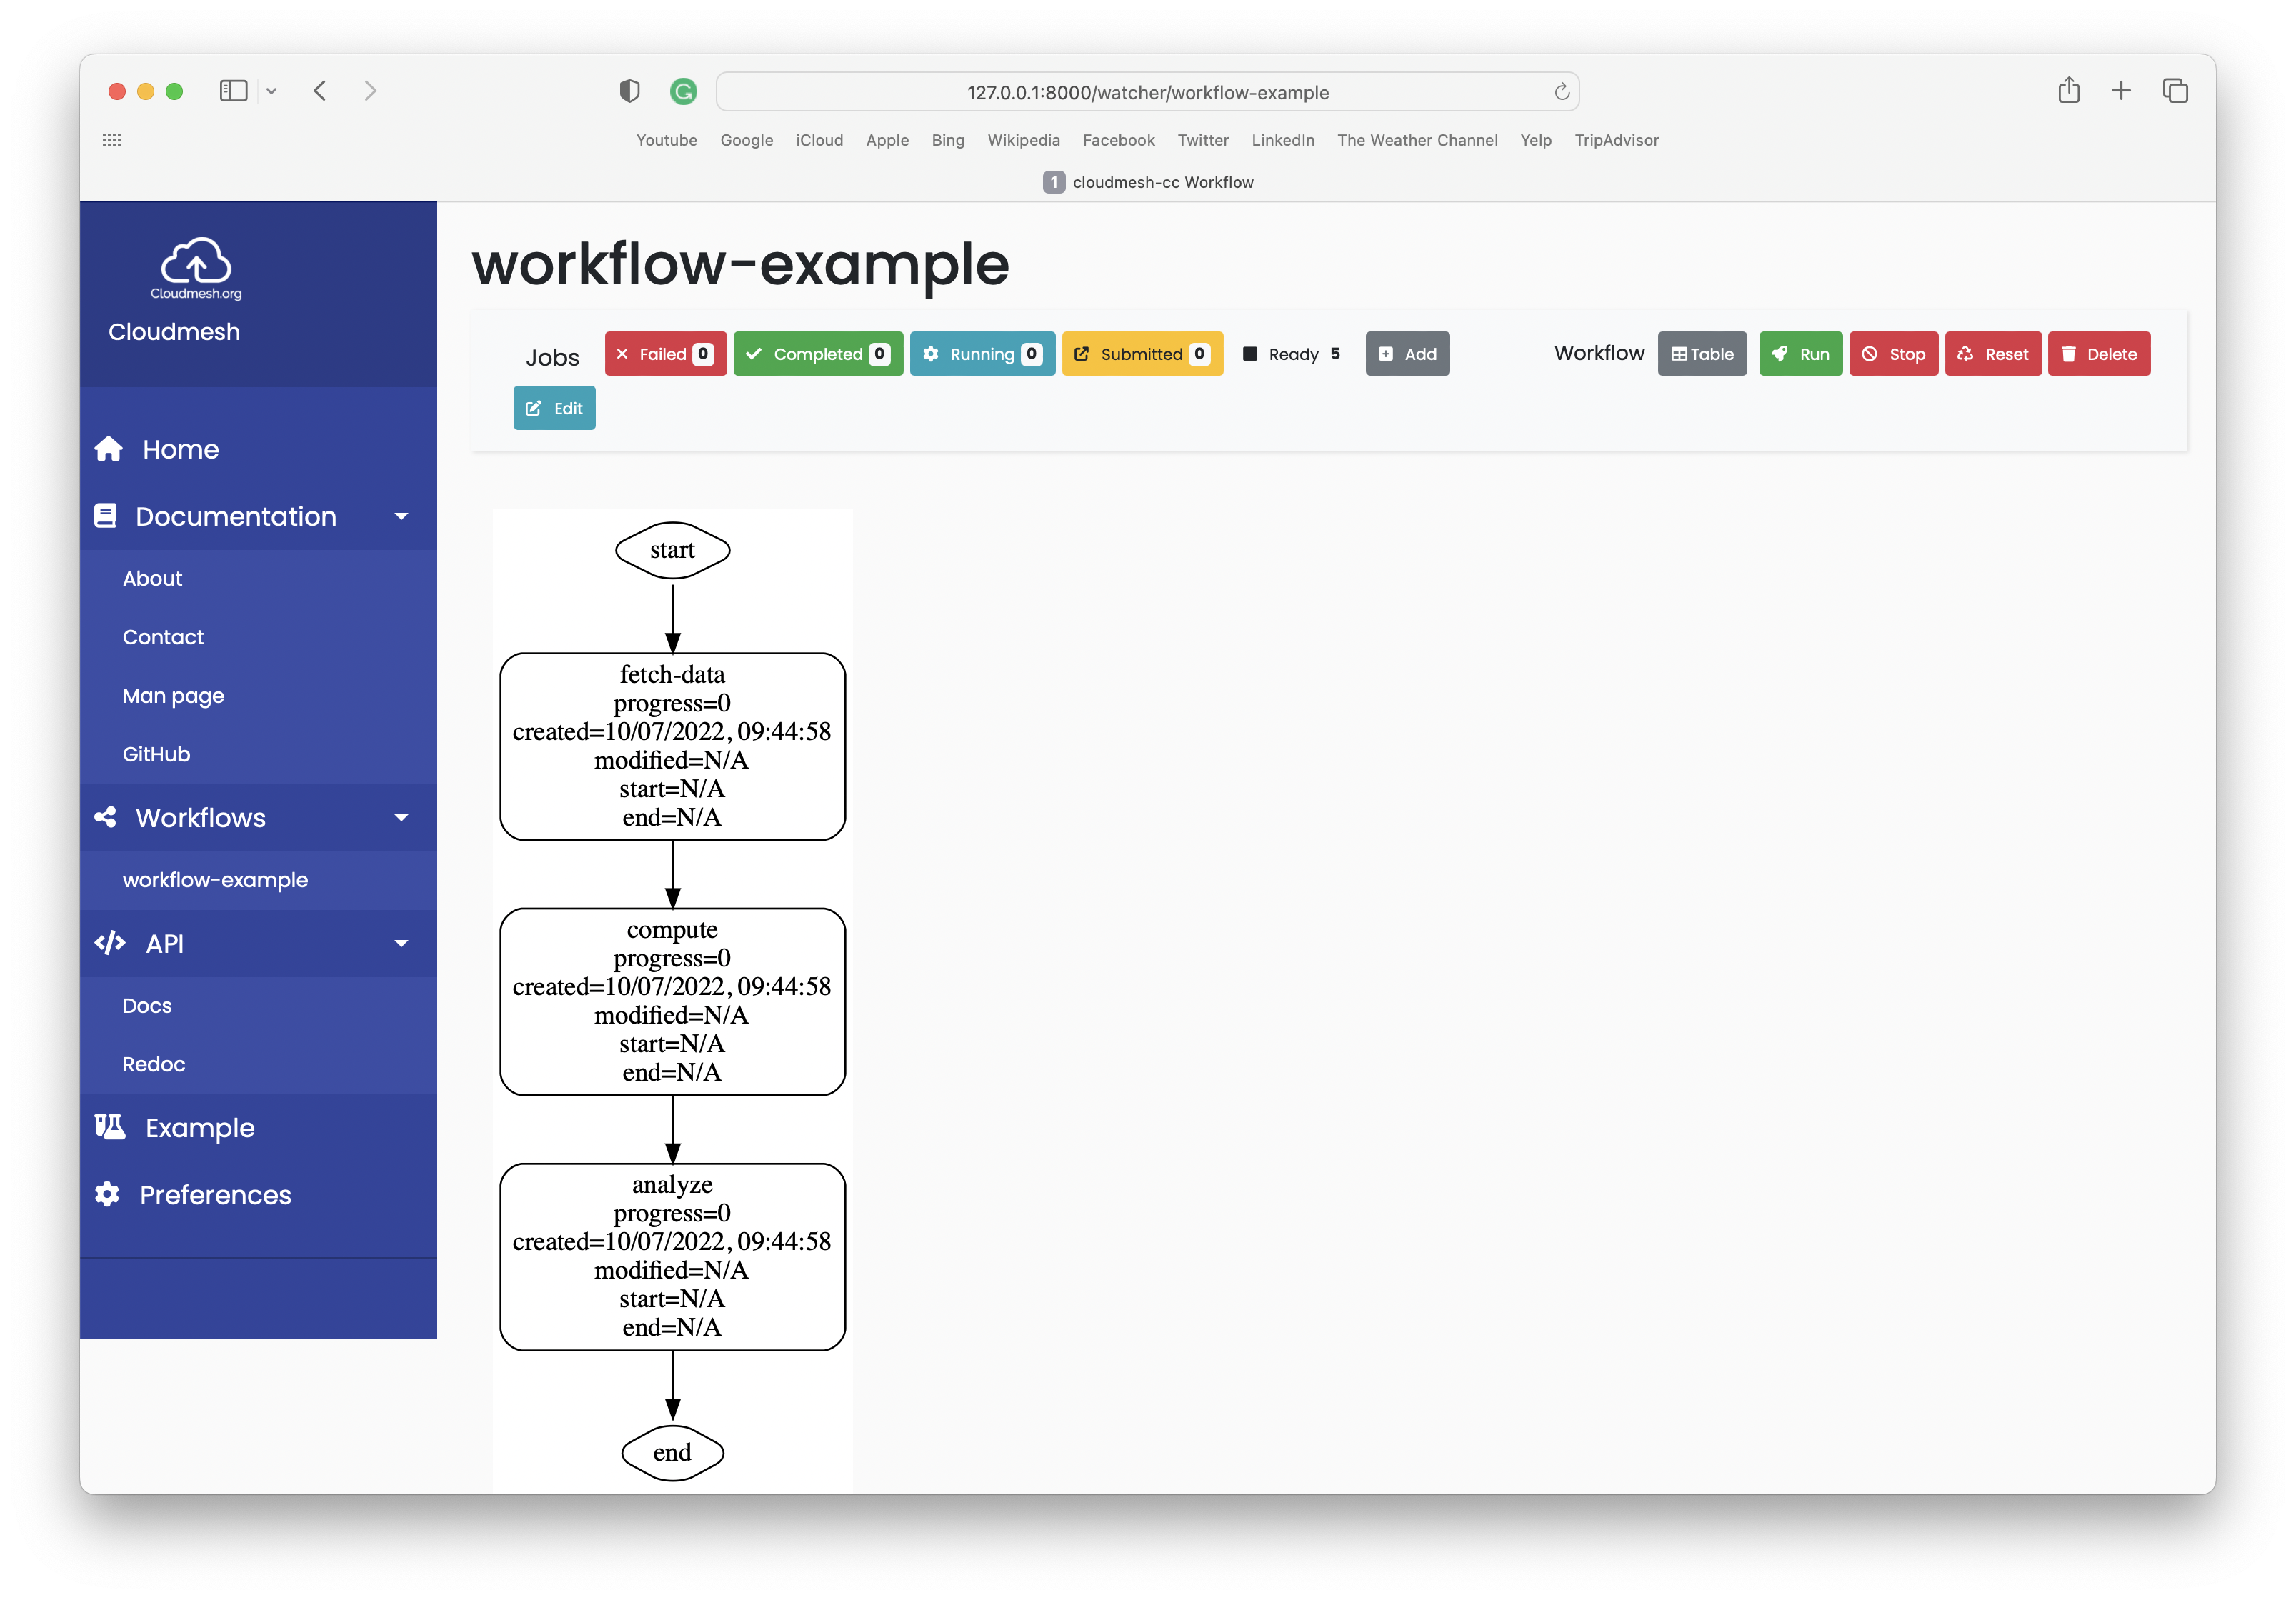
\includegraphics[width=1.05\columnwidth]{images/service-graph.png}
  \caption{Cloudmesh cc workflow graph view}}
\label{fig:graph}
\end{figure}



\subsection{Run the workflow}\label{run-the-workflow}

To run a workflow, you can use the various interfaces to do so. As an
example we will showcase here how to run is in the service mode bey
either the GUI or a curl call.

\paragraph{GUI.} To run, navigate to homepage at
\texttt{http://127.0.0.1:8000/} and click the workflow-example on the
left side. Then click Run.


\paragraph{Curl.} to run a workflow with curl please use

\begin{minted}[breaklines]{bash}
$ curl -X 'GET' 'http://127.0.0.1:8000/workflow/run/workflow-example
?show=True' -H 'accept: application/json'
\end{minted}%$

\paragraph{RESTWorkflow API}

To run the workflow with the Python cloudmesh REST API, please use the code

\begin{minted}[breaklines]{python} 
from cloudmesh.cc.workflowrest import RESTWorkflow
rest = RESTWorkflow()
result = rest.run_workflow('workflow-example')
\end{minted}

\paragraph{Python request API.} To run the workflow with the Python
request API, please use the code

\begin{minted}[breaklines]{python}
import requests
url = f'http://127.0.0.1:8000/workflow/run/workflow-example?show=True'
r = requests.get(url)
print(r)
\end{minted}








\FILE{interfaces.tex}

\section{Cloudmesh-cc Interfaces}

In this section, we explain the various ways of interfacing with
cloudmesh-cc that are part of our design (see Figure~\ref{fig:arch}).

It is important to note that we have a {\em command line mode} that
interfaces directly with the backends while not requiring a
service. This includes an easy-to-use Python API.

In addition, we have used this API to implement a {\em service mode}, so we can
stand up a REST service as well as a GUI that can be accessed through a Web browser.
Please note that the service mode can also be accessed through the command line
in a terminal. To distinguish how we operate cloudmesh-cc, we use the term
{\em mode} to delineate it from a command that is entered in a terminal to
query the status of the workflow.

We will now discuss these interfaces in more detail and also showcase
how we can access them.


\subsection{Python API}

Cloudmesh-cc is implemented in Python. Extensive documentation is
available in GitHub and, using GitHub Actions, it is automatically
updated~\cite{github-cloudmesh-cc}. We distinguish two main classes
that are easy to use. The first is a {\em Job class} that can be
adapted to include new computational resource types for executing
jobs. The second is a {\em Workflow class} to coordinate the execution
of multiple jobs. Selected methods of the Job class include are listed
in Figure~\ref{fig:code-job}. Important to note is that the code for
the scripts are all managed locally, and a synchronization step is
invoked prior to one running the job to assure that the latest script
and code to be executed on the compute resource is available.

The most important part of using the Workflow Python API is showcased
in Figure~\ref{fig:code-job}, where we explain how easy it is to set
up a workflow with the Python API.

\begin{figure}[!h]
\begin{minted}[breaklines]{bash}
class Job:
   ...
   def clear():
      """Clear job progress."""
   def create(filename=None, script=None, exec=None):
      """Create a template for the script with progress."""
   def get_log(refresh=True):
      """Get the log of the job."""
   def get_pid(refresh=False):
      """Get the pid that the job is running within determined by the compute resource it is running on."""
   def get_progress(refresh=False):
       """Get the progress of the job from the compute resource."""
   def get_status(refresh=False):
       """Get the status of the job."""
   def kill():
       """Kill the job."""
   def run():
       """Run the job."""
   def sync():
       """Synchronise the current directory with the remote. Copies the shell script to the experiment directory and ensures that the file is copied with the sync command."""
   def watch(period=10):
       """Watch the job and check for changes in the given period."""
\end{minted}
\caption{Pseudo code for the Job class with selected methods.}
\label{fig:code-job}

\bigskip

\begin{minted}[breaklines]{bash}
class Workflow:
    ...
    def add_dependencies(dependency):
        """Add a job dependency to the workflow (and the graph)."""
    def add_dependency(source, destination):
        """Add a job dependency to the workflow (and the graph)."""
    def add_job( ... ):
        """Add a job to the workflow with appropriate parameters."""
    def display(filename=None, name='workflow', first=True):
        """Show the graph of the workflow."""
    def job(name):
        """Return the details of a job within the workflow."""
    def load(filename, clear=True):
        """Load the workflow."""
    def remove_job(name, state=False):
        """Remove a particular job from the workflow."""
    def remove_workflow():
        """Delete workflow from the local file system."""
    def run_parallel( ... ):
        """Run a workflow in a parallel fashion."""
    def run_topo(order=None, dryrun=False, show=True, filename=None):
        """Run the workflow in a topological order."""
    def save(filename=None):
        """Save the workflow."""
    def save_with_state(filename, stdout=False):
        """Save the workflow with state."""
    def sequential_order():
        """Return a list of the topological order of the workflow."""
    property table:
        """Return a table of the workflow."""
    def update_progress(name):
        """Manually update the progress of a job according to its log file."""
    def update_status(name, status):
        """Manually update a job’s status."""
\end{minted}
\caption{Pseudo code for the Job class with selected methods.}
\label{fig:code-workflow}
\end{figure}


\begin{figure}[htb]
\begin{minted}[breaklines]{bash}
    w = Workflow(name="workflow-analyze")
    # load a preexisting workflow
    # w.load(filename="source.yaml")
    
    # add jobs and dependencies explicitly
    w.add_job(name="fetch-data",
              exec="hostname",
              host="supercomputer-a", # defined in .ssh
              label="{name}\nprogress={progress}",
              kind="local",
              status="ready",
              progress=0)
    w.add_job(name="compute", command="... TBD ...")
    w.add_job(name="analyze", command="... TBD ...")
    w.add_dependencies(
              dependency="start,fetch-data,compute,analyze")
    w.run_topo()
\end{minted}
\caption{Pseudo code for the Job class with selected methods.}
\label{fig:code-workflow-example}

\bigskip

\begin{minted}[breaklines]{bash}
      cms cc workflow add [--name=NAME] [--job=JOB] ARGS...
      cms cc workflow add [--name=NAME] --filename=FILENAME
      cms cc workflow delete [--name=NAME] [--job=JOB]
      cms cc workflow list [--name=NAME] [--job=JOB]
      cms cc workflow run [--name=NAME] [--job=JOB] [--filename=FILENAME]
      cms cc workflow [--name=NAME] --dependencies=DEPENDENCIES
      cms cc workflow status --name=NAME [--output=OUTPUT]
      cms cc workflow graph --name=NAME
\end{minted}
\caption{Command line interface to the workflow in terminal mode.}
\label{fig:code-workflow-commandline}

\bigskip

\begin{minted}[breaklines]{bash}
      cms cc start [-c] [--reload] [--host=HOST] [--port=PORT]
      cms cc stop
      cms cc status
      cms cc workflow service add [--name=NAME] FILENAME
      cms cc workflow service list [--name=NAME] [--job=JOB]
      cms cc workflow service add [--name=NAME] [--job=JOB] ARGS...
      cms cc workflow service run --name=NAME
\end{minted}
\caption{Command line interface to the workflow in service mode.}
\label{fig:code-workflow-service-commandline}.

% \bigskip

{\centering
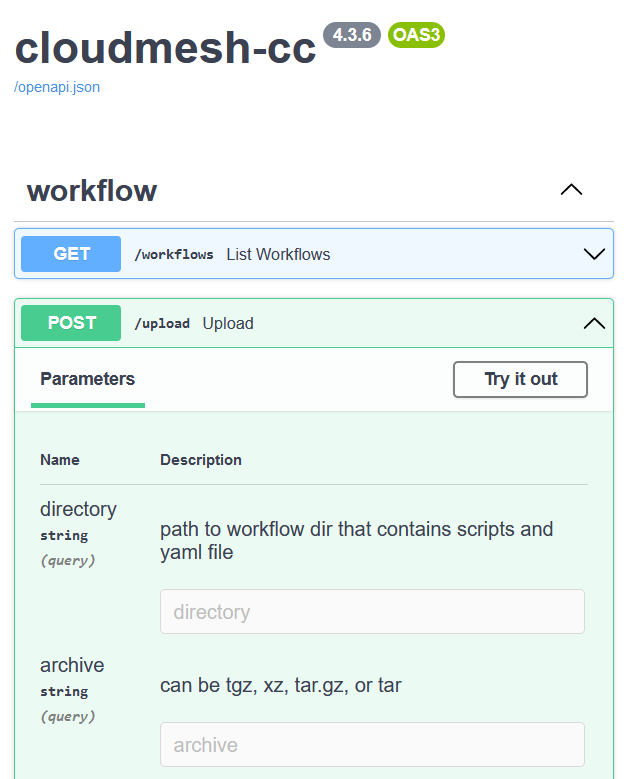
\includegraphics[width=0.52\columnwidth]{images/upload_api.png}
}
\caption{Browser API GUI for Cloudmesh Compute Cluster.}

\label{fig:openapi}

\end{figure}


\subsection{Commandline Mode}

The command line mode is an implementation that does not use a backend
service. It runs in the terminal until the workflow is completed. All
states of the jobs are managed on the compute service on which the job
is run and the status is replicated into the client on demand. This
allows easy reporting of the status through a table and a graph
display using client-based rendering tools. The various commands to
interact with it on the command line are shown in
Figure~\ref{fig:code-workflow-commandline}.


\subsection{Service Mode}

The Python API has been used to implement a REST service. To easily
interact with the REST service we have also added a couple of
convenient commands one can issue from a terminal. They are listed in
Figure~\ref{fig:code-workflow-service-commandline}. It is clear from
these methods that starting, stopping, and getting the status of the
service is very easy. In contrast to the command line mode, this
service mode has an additional keyword {\em service} to interact with
the rest service.

Certainly one can also directly interact with the REST service API for
this service. For ease of use, we have exposed the interface through
an OpenAPI specification that is available to the user as shown in
Figure~\ref{fig:openapi}.

Thus, other tools such as curl or other languages supporting URL
requests can be used. A curl example to list the workflow
specifications uploaded to the service is as follows:

\begin{minted}[breaklines]{bash}
$ curl -X 'GET'  'http://127.0.0.1:8000/workflows' -H 'accept: application/json'
\end{minted}
% $

As we use a REST service, we can also easily upload the workflow
through a Python-enabled REST call. We will use Python requests to
demonstrate this upload feature. To showcase the various ways to
access the service, we focus on uploading a tar file that contains the
workflow as well as the scripts or programs used in the workflow. The
tar file is called {\em workflow.tar}.

To also allow programming against the REST service in Python, a Python
API similar to that of the command line mode is
available. Figure~\ref{fig:code-workflow-rest-commandline} showcases
this API.

To simplify interaction with the REST service, we create a special
{\em RESTWorkflow class} that is similar to the command module API,
but instead uses the REST interface to the service rather than direct
communication with the command client API.

The user can also simply use the requests module in Python to
interface with the API. Figure~\ref{fig:code-workflow-requests}
demonstrates how to use requests to upload a workflow by using an
archive file that contains the YAML configuration file and the
scripts.

\begin{figure}[t]
\begin{minted}[breaklines]{bash}
class RESTWorkflow
    ...
    def add_job(workflow_name, **kwargs):
        """Add a job to the workflow."""
    def delete_workflow(workflow_name, job_name=None):
        """Delete a workflow by using REST."""
    def get_workflow(workflow_name, job_name=None):
        """Retrieve a workflow by using REST."""
    def list_workflows():
        """Return a list of workflows that is found within
           the server."""
    def run_workflow( ... ):
        """Run a workflow by using REST."""
    def upload_workflow( ... ):
        """Upload a workflow by using REST."""
\end{minted}
\caption{Pseudo code for the Job class with selected methods.}
\label{fig:code-workflow-rest-commandline}

\bigskip

\begin{minted}[breaklines]{python}
import requests
r = requests.post(
      'http://127.0.0.1:8000/workflow?archive=workflow-example.tar')
print(r.text)
\end{minted}
\caption{Upload to the REST service with Python requests.}
\label{fig:code-workflow-requests}

\bigskip

\begin{minted}[breaklines]{bash}
$ curl -X 'POST' 'http://127.0.0.1:8000/ workflow?archive=workflow-example.tar'                           -H 'accept: application/json' -d ''
\end{minted}
% $
\caption{Upload to the REST service with curl.}
\label{fig:code-workflow-curl}

\end{figure}


\subsection{Webservice GUI}

A convenient Web service is included in Cloudmesh cc. It allows the
user to manage and visualize the status of workflows through a Web
browser interface. At this time, the focus is that the interface can
be run by a single user on the local machine. This allows remote
executions of workflow nodes run completely independent from cloudmesh
cc and interaction is possible in asynchronous mode.

As the service is using also an OpenAPI 2.0 specification, the
workflow can also be uploaded implicitly through the specification
GUI. Navigate to {\scriptsize \texttt{http://127.0.0.1:8000/docs}} and
use the POST Upload method. Then click \texttt{Try\ it\ out} and enter
the location of the tar file, followed by clicking {\em Execute}.

Obviously, any REST service or REST API can be used, allowing the user
to interface to it from different programming languages or frameworks.

The web server provides a more customizable, easy-to-use interface for
the Workflow class which can be started, viewed and stopped with the
appropriate command line.

\begin{minted}[breaklines]{bash}
  $ cms cc start
  $ cms cc view
  $ cms cc stop
\end{minted}
%$

The view can also be achieved by opening the 
the link {\scriptsize\texttt http://127.0.0.1:8000/}.

The browser provides an interface to view preexisting workflows in
both a DataTable format and as a graph format. Both views will update
in a live, automatic fashion as the workflows are run, reporting
dynamic job status and progress.

For a quick and easy example of leveraging this GUI interface, click
on the Example tab in the left-hand sidebar. Then, a workflow-example
will appear underneath Workflows. Click on the workflow-example and
run the workflow by clicking the green Run button in the top-right. As
the workflow runs, the user is able to click on the Graph button to
view the graph interface (see Figure~\ref{fig:graph}) and back to the
Table button for the table interface (see Figure~\ref{fig:table}), as
desired, to view the workflow's progression.


\begin{figure}[htb]
{\centering
  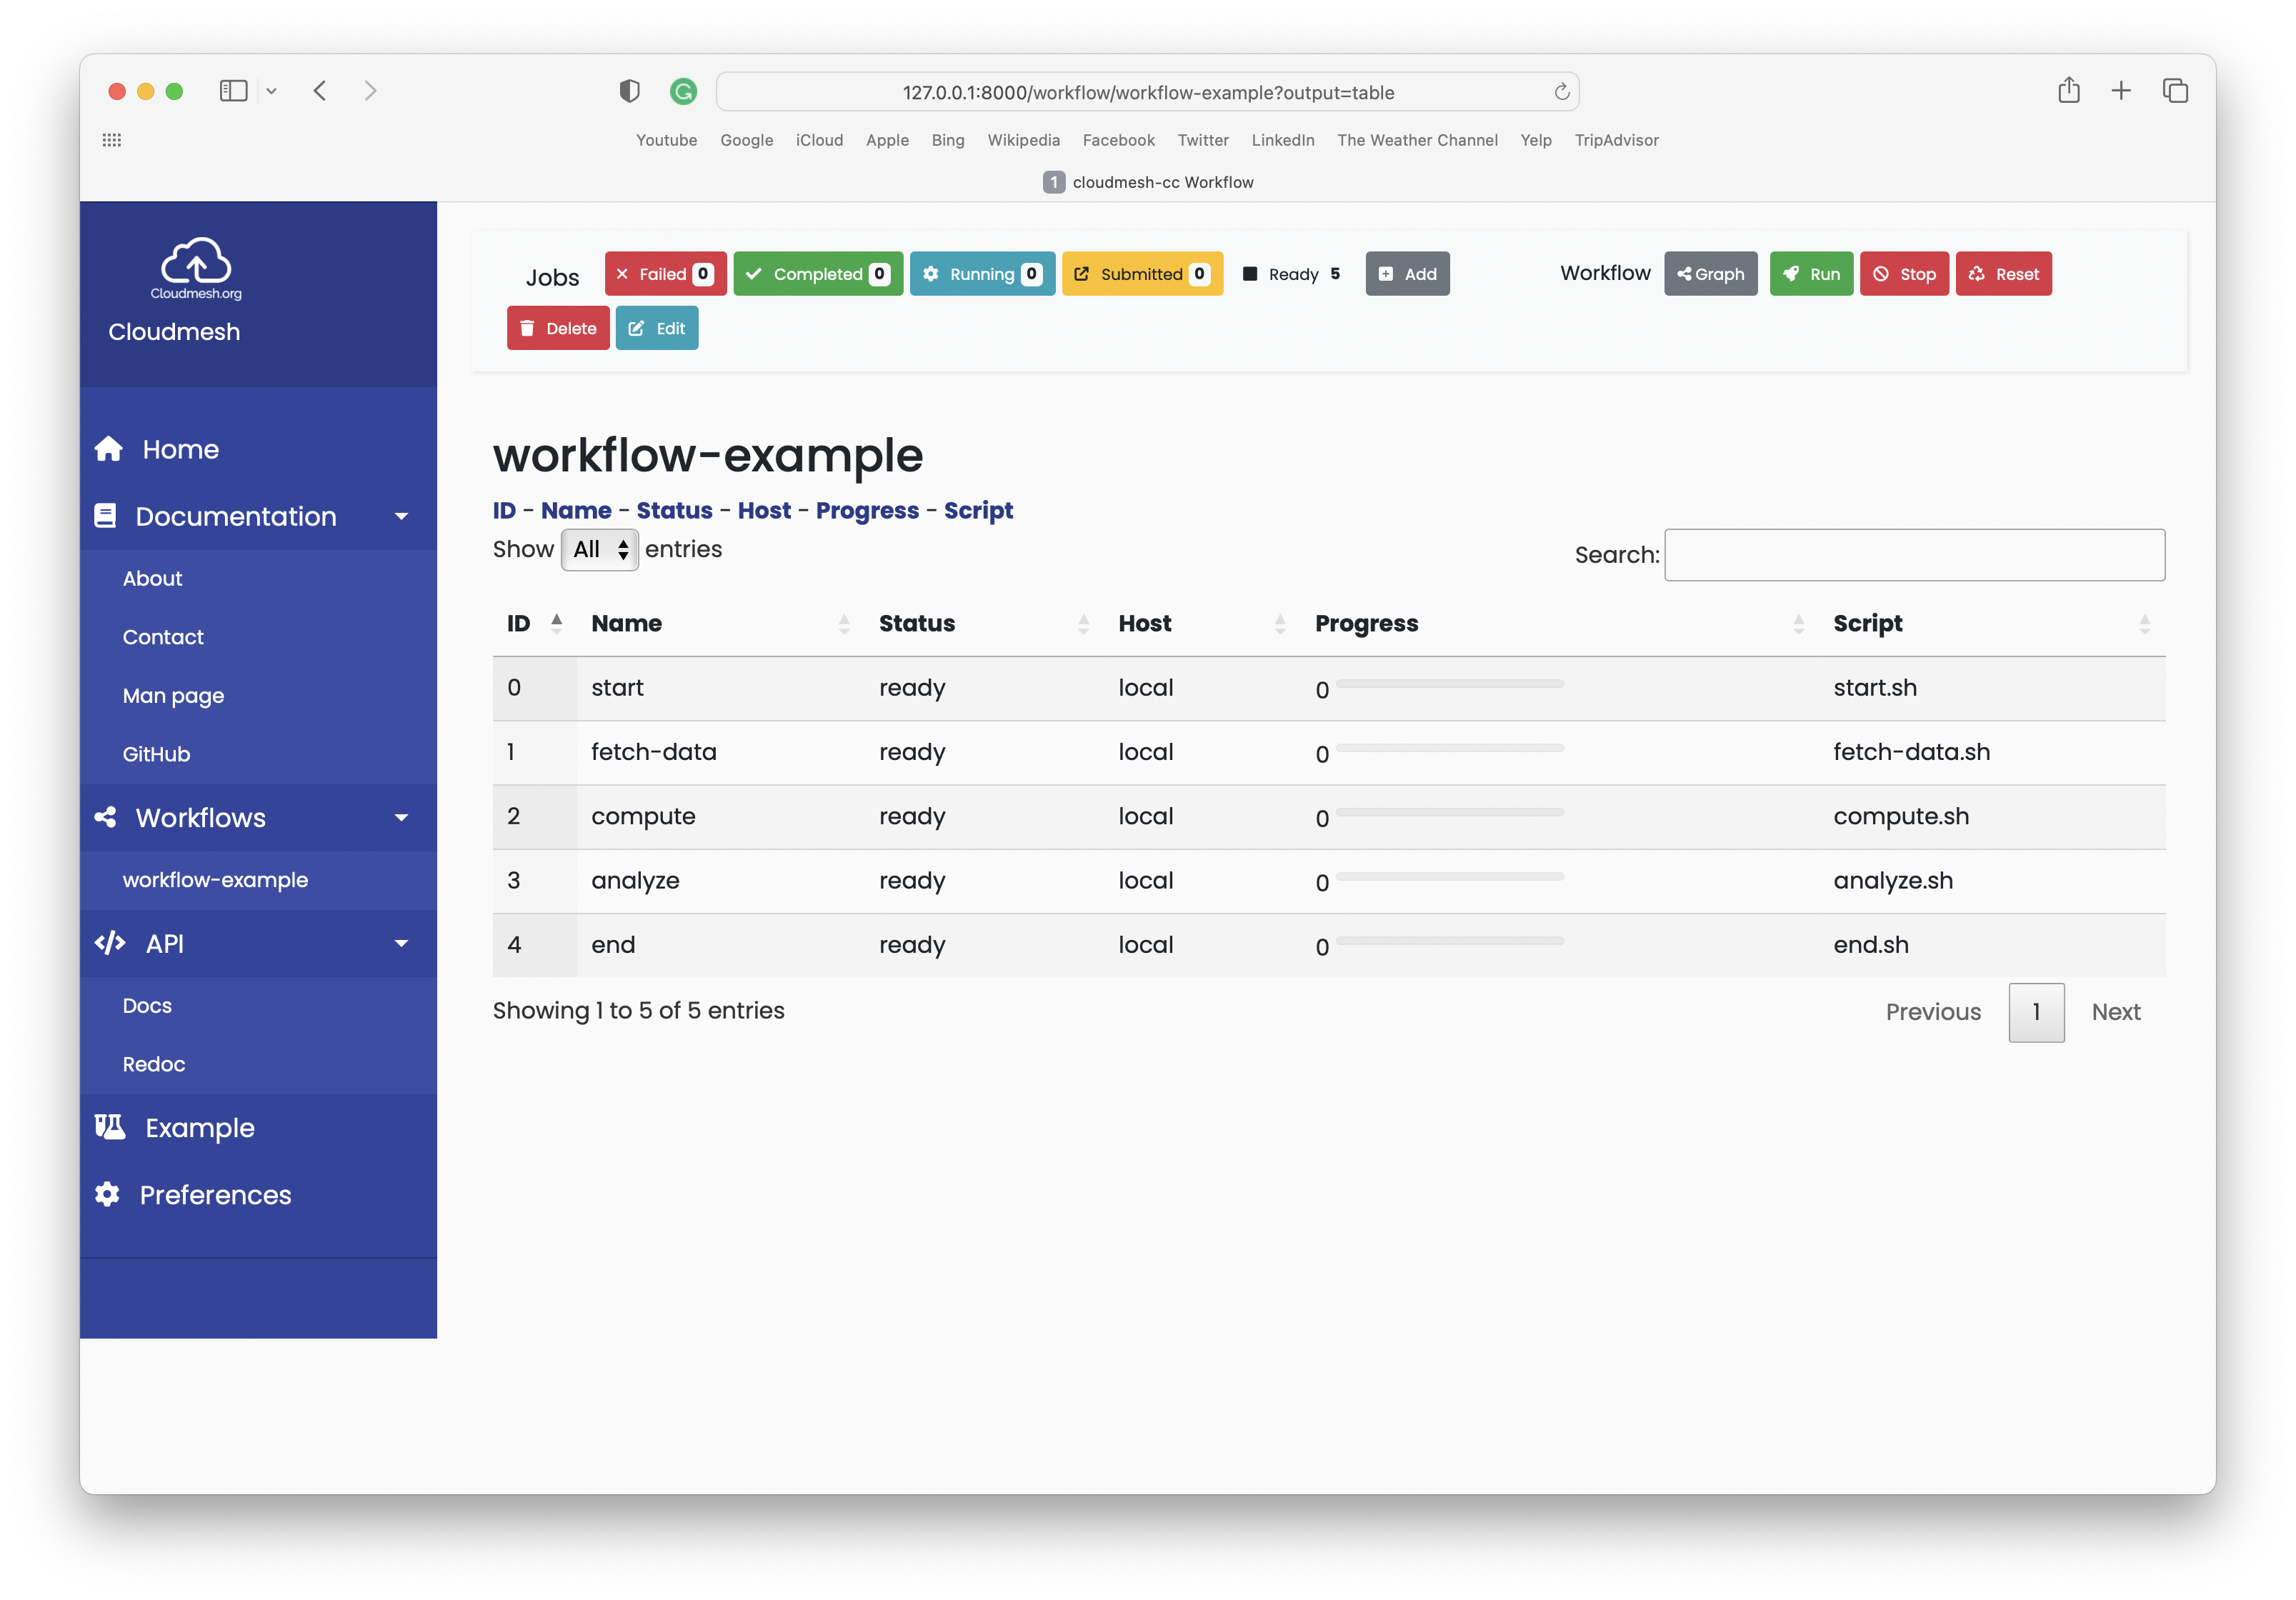
\includegraphics[width=1.0\columnwidth]{images/service-table.png}
}
\vspace{-1.0cm}
\caption{Cloudmesh cc workflow table view.}\label{fig:table}

\bigskip
{\centering
  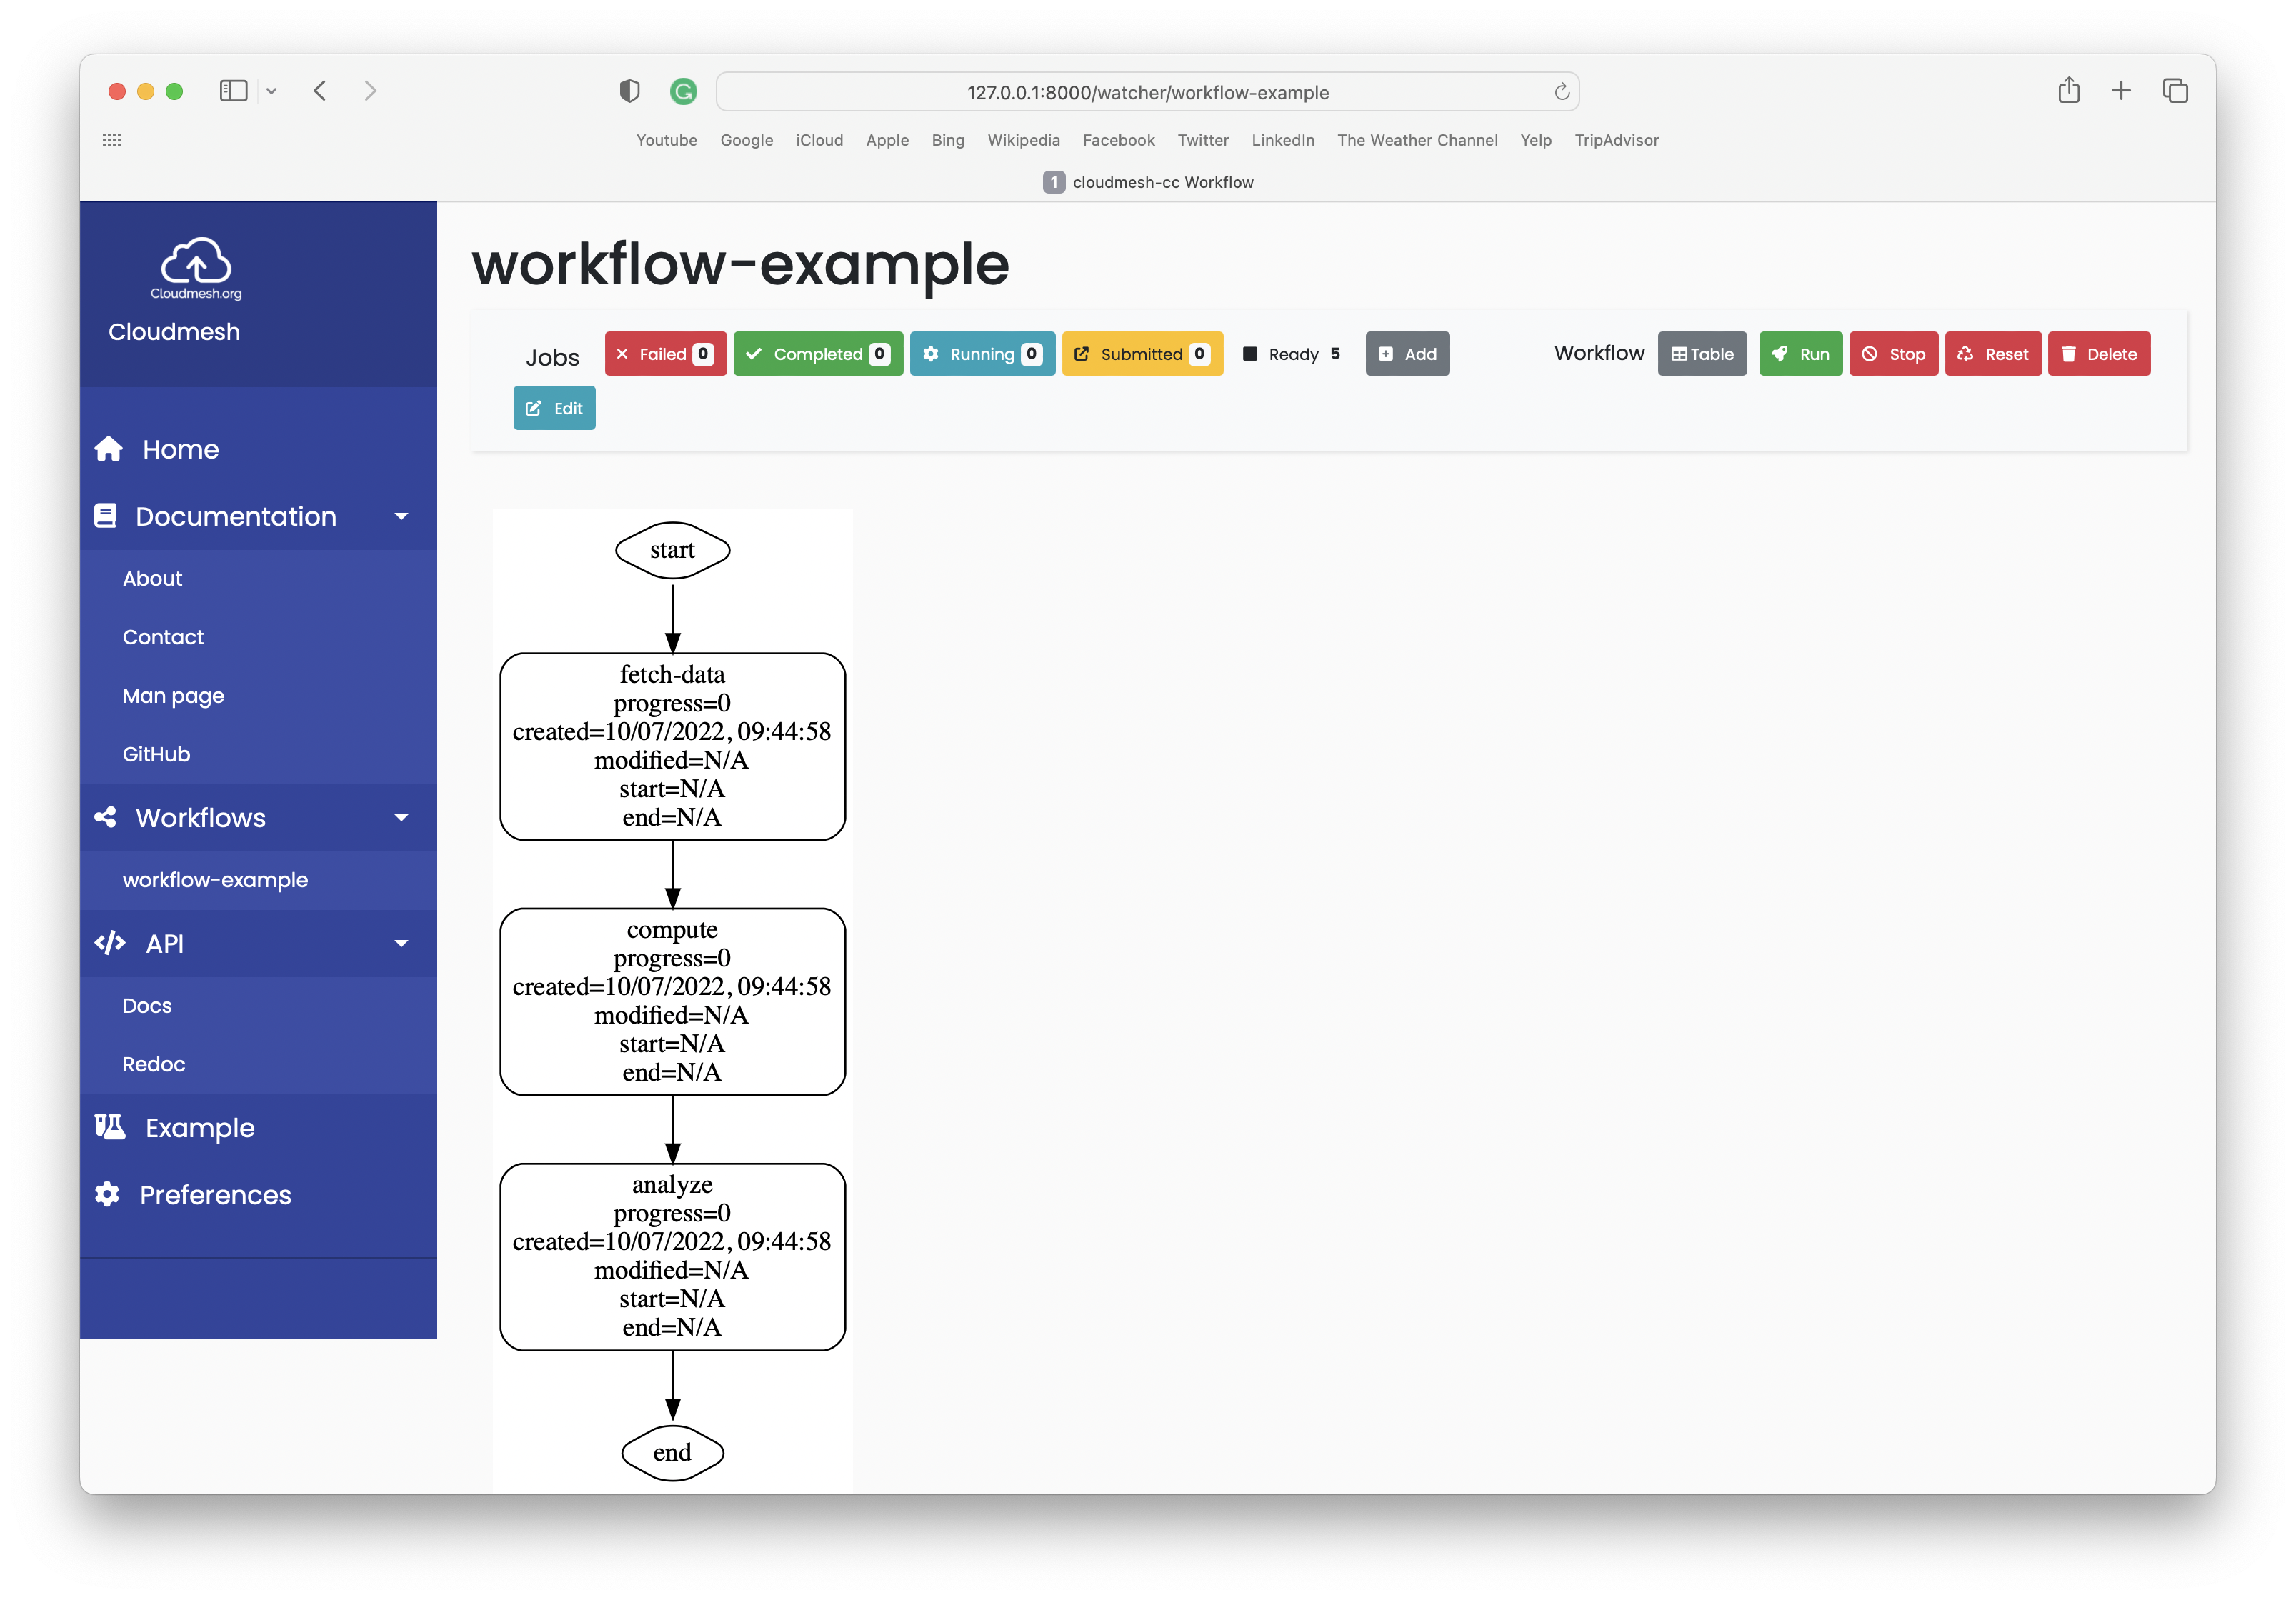
\includegraphics[width=1.0\columnwidth]{images/service-graph.png}
 }
\vspace{-1.0cm}
 \caption{Cloudmesh cc workflow graph view.}

\label{fig:graph}
\end{figure}



\subsection{Run the workflow}\label{run-the-workflow}

The workflow can be run easily via the GUI. We added a special set of
buttons to the workflow table and graph display to simplify running of
the workflow.  Certainly, the workflow can also be activated while
calling the appropriate REST call, either through, Python, the OpenAPI
docs page, or, for example, a curl call such as where {\em
workflow-example} is the name of the workflow to be
executed. Figure~\ref{fig:workflow-run-a}-\ref{fig:workflow-run-c}
showcases various methods to run the example workflow.


\begin{figure}[htb]

\begin{minted}[breaklines]{bash}
$ curl -X 'GET' 'http://127.0.0.1:8000/workflow/run/workflow-example?show=True' -H 'accept: application/json'
\end{minted}
% $
\flushleft
\caption{\parindent0pt Running the example workflow with curl.}
\label{fig:workflow-run-a}
\bigskip

\begin{minted}[breaklines]{python} 
from cloudmesh.cc.workflowrest import RESTWorkflow
rest = RESTWorkflow()
result = rest.run_workflow('workflow-example')
\end{minted}
\caption{Running the example workflow with cloudmesh RESTWorkflow API.}
\label{fig:workflow-run-b}
\bigskip

\begin{minted}[breaklines]{python}
import requests
url = f'http://127.0.0.1:8000/workflow/run/workflow-example?show=True'
r = requests.get(url)
print(r)
\end{minted}

\caption{Running the example workflow with requests API.}
\label{fig:workflow-run-c}

\end{figure}









% \FILE{cloudmesh.tex}

\section{Other Cloudmesh Features}

Cloudmesh comes with a sophisticated package management system, allowing to integrate packages on demand targeting varipus providers ond capabilities including a build in command shell and not just aonly a commanline tool.  Cloudmesh was first develped as a hybrid cloud API, commandline and command shell framework. It provided interfaces to AWS, Azure, Google, and OpenStack clouds for virtual machine\footnote{cloudmesh also provded support for clouds that are no longer supported such as Eucalyptsus and open cirrus. Academic clouds such as Chameloncloud were also supported.} and data file services. It is characterized be defining default templates for virtual machine management on these clouds. Hence it was possible to switch with only a view commands between clouds and stage virtual machines on them such as demonstarted in Figure~\ref{fig:cms}.

\begin{figure}[htb]

\begin{minted}[breaklines]{bash}
$ cms vm start --cloud aws
$ cms vm start --cloud azure
\end{minted}

  \caption{Simple VM managegment for hybrid clouds}
\label{fig:cms}.
\end{figure}  

In addition we have also developed a pacage called GAS that addresses the creation of analytics REST services from python functios. This package was developed to address the problem that integrating deployment frameworks in the age of cloud computing is often out of reach for domain experts.  GAS is a simple frameworks allowing even non-experts to deploy and host services in the cloud. To avoid vendor lock-in it supports multiple vendors through the use of cloudmesh vm management \cite{las21-gas}.


\FILE{cloudmesh.tex}

\section{Other Cloudmesh Features}

Cloudmesh comes with a sophisticated package management system,
allowing the integration of packages on demand targeting various providers
and capabilities including a built-in command shell (not just only
a command line tool). Cloudmesh was first developed as a hybrid cloud
API, command line and command shell framework. It provided interfaces
to AWS, Azure, Google, and OpenStack clouds for virtual
machine\footnote{cloudmesh also provided support for clouds that are no
longer supported such as Eucalyptus and Open Cirrus. Academic clouds
such as Chameleon Cloud were also supported.} and data file services. It
is characterized by defining default templates for virtual machine
management on these clouds. Hence, it was possible to switch between clouds
with only a few commands and stage virtual machines on them, such
as with the commands demonstrated in Figure~\ref{fig:cms}.

\begin{figure}[htb]

\begin{minted}[breaklines]{bash}
$ cms vm start --cloud aws
$ cms vm start --cloud azure
\end{minted}

  \caption{Simple VM management for hybrid clouds}
\label{fig:cms}.
\end{figure}  

In addition, we have developed a package called GAS that addresses
the creation of analytics REST services from Python functions. This
package was developed to address the problem that integrating
deployment frameworks in the age of cloud computing is often out of
reach for domain experts. GAS is a simple framework allowing even
non-experts to deploy and host services in the cloud. To avoid vendor
lock-in, it supports multiple vendors through the use of cloudmesh vm
management~\cite{las21-gas}.


% \FILE{applications.tex}

\section{Workflow Applications}

We have applied the workflow system on a number of appliactions. All workflows for these applications are avaialable in our GitHub and can be adapted easily.
This includes the Cloudmask and MNIST application workflows which we describe next in more details.



\FILE{applications.tex}

\section{Workflow Applications}

We have applied the workflow system on a number of applications. All
workflows for these applications are available in our GitHub and can
be adapted easily. This includes the Cloudmask and MNIST application
workflows which we describe next in more details.




% \section{Cloudmask Workflow}\label{cloudmask-workflow}

Cloudmesh cc comes with an example workflow that runs Cloudmask, which
is a program that develops a model to classify sections of satellite
images. Information regarding Cloudmask can be found at
\url{https://github.com/laszewsk/mlcommons/tree/main/benchmarks/cloudmask\#readme}

\subsection{Running the Cloudmask Workflow on
Rivanna}\label{running-the-cloudmask-workflow-on-rivanna}

To execute the workflow on UVA's HPC supercomputer, Rivanna, first
ensure that your UVA Computing ID is set with the following command,
replacing the X's with your ID:

\begin{verbatim}
me@mycomputer $ cms set username=XXXXXX
\end{verbatim}

Then, connect to the UVA Anywhere VPN and then download the satellite
data into your
\href{https://www.rc.virginia.edu/userinfo/storage/non-sensitive-data/\#scratch}{scratch}
directory on Rivanna:

\begin{verbatim}
me@mycomputer $ cms vpn connect
me@mycomputer $ ssh rivanna
rivanna $ cd /scratch/$USER
rivanna $ git clone https://github.com/laszewsk\
/mlcommons.git
rivanna $ cd mlcommons/benchmarks/cloudmask\
/target/rivanna
rivanna $ make data
# downloading the data will take a while.
rivanna $ exit
\end{verbatim}

Next, clone the \texttt{mlcommons} repository on your local machine and
run the workflow:

\begin{verbatim}
me@mycomputer $ cd ~/cm
me@mycomputer $ git clone https://github.com\
/laszewsk/mlcommons.git
me@mycomputer $ cd mlcommons
me@mycomputer $ pytest -v -x --capture=no \ 
benchmarks/cloudmask/target/rivanna/run_cloudmask\
_workflow.py
\end{verbatim}

The workflow iterates through the five GPUs available on Rivanna---
A100, V100, P100, RTX2080, and K80--- and runs the program three times
on each GPU. Each run trains the model with 10, 30, and 50 epochs for
benchmarking.

Upon completing a run, the logs and benchmarks of the program can be
found in the target folder:

\begin{verbatim}
me@mycomputer $ ssh rivanna
rivanna $ cd /scratch/$USER/mlcommons\
/benchmarks/cloudmask/target
\end{verbatim}

Additionally, the generated \texttt{.h5} model file can be found in the
home directory:

\begin{verbatim}
 rivanna $ cd ~/sciml_bench/outputs/slstr_cloud/
 \end{verbatim}

The program may take a while to run if the resources on Rivanna are
being used by other jobs.


\FILE{Cloudmask.tex}

\subsection{MLCommons Cloudmask Workflow}
\label{cloudmask-workflow}

Cloudmask is a program that develops a model to classify sections of
satellite images as either containing clouds or clear sky by using
machine learning. This is beneficial for temperature measurement and
meteorology. Information regarding Cloudmask can be found on its
GitHub page~\cite{www-cloudmask}. One of our goals is to run
Cloudmask for benchmarking. As benchmarking Cloudmask requires
several phases and scripts, including a mixture of shell scripts and
Python scripts, leveraging Cloudmesh-cc provides a much easier runtime
instead of manually issuing many commands at a terminal. We have
created a sample workflow the runs a coordinated workflow across a
number of hybrid resources. This includes an HPC computer at
University of Virginia called Rivanna, as well as two desktop
computers. This workflow can easily be adapted to include other
machines. In this particular workflow, we execute the benchmarks on a
number of different CUDA cards (see Figure~\ref{fig:cloudmaskwf}. For
Rivanna, the code also utilizes our cloudmesh-vpn component that
provides the ability to connect to the UVA VPN from Python, then
fetches the data and executes the various benchmarks once the data is
available.

\begin{figure*}[htb]
\centering
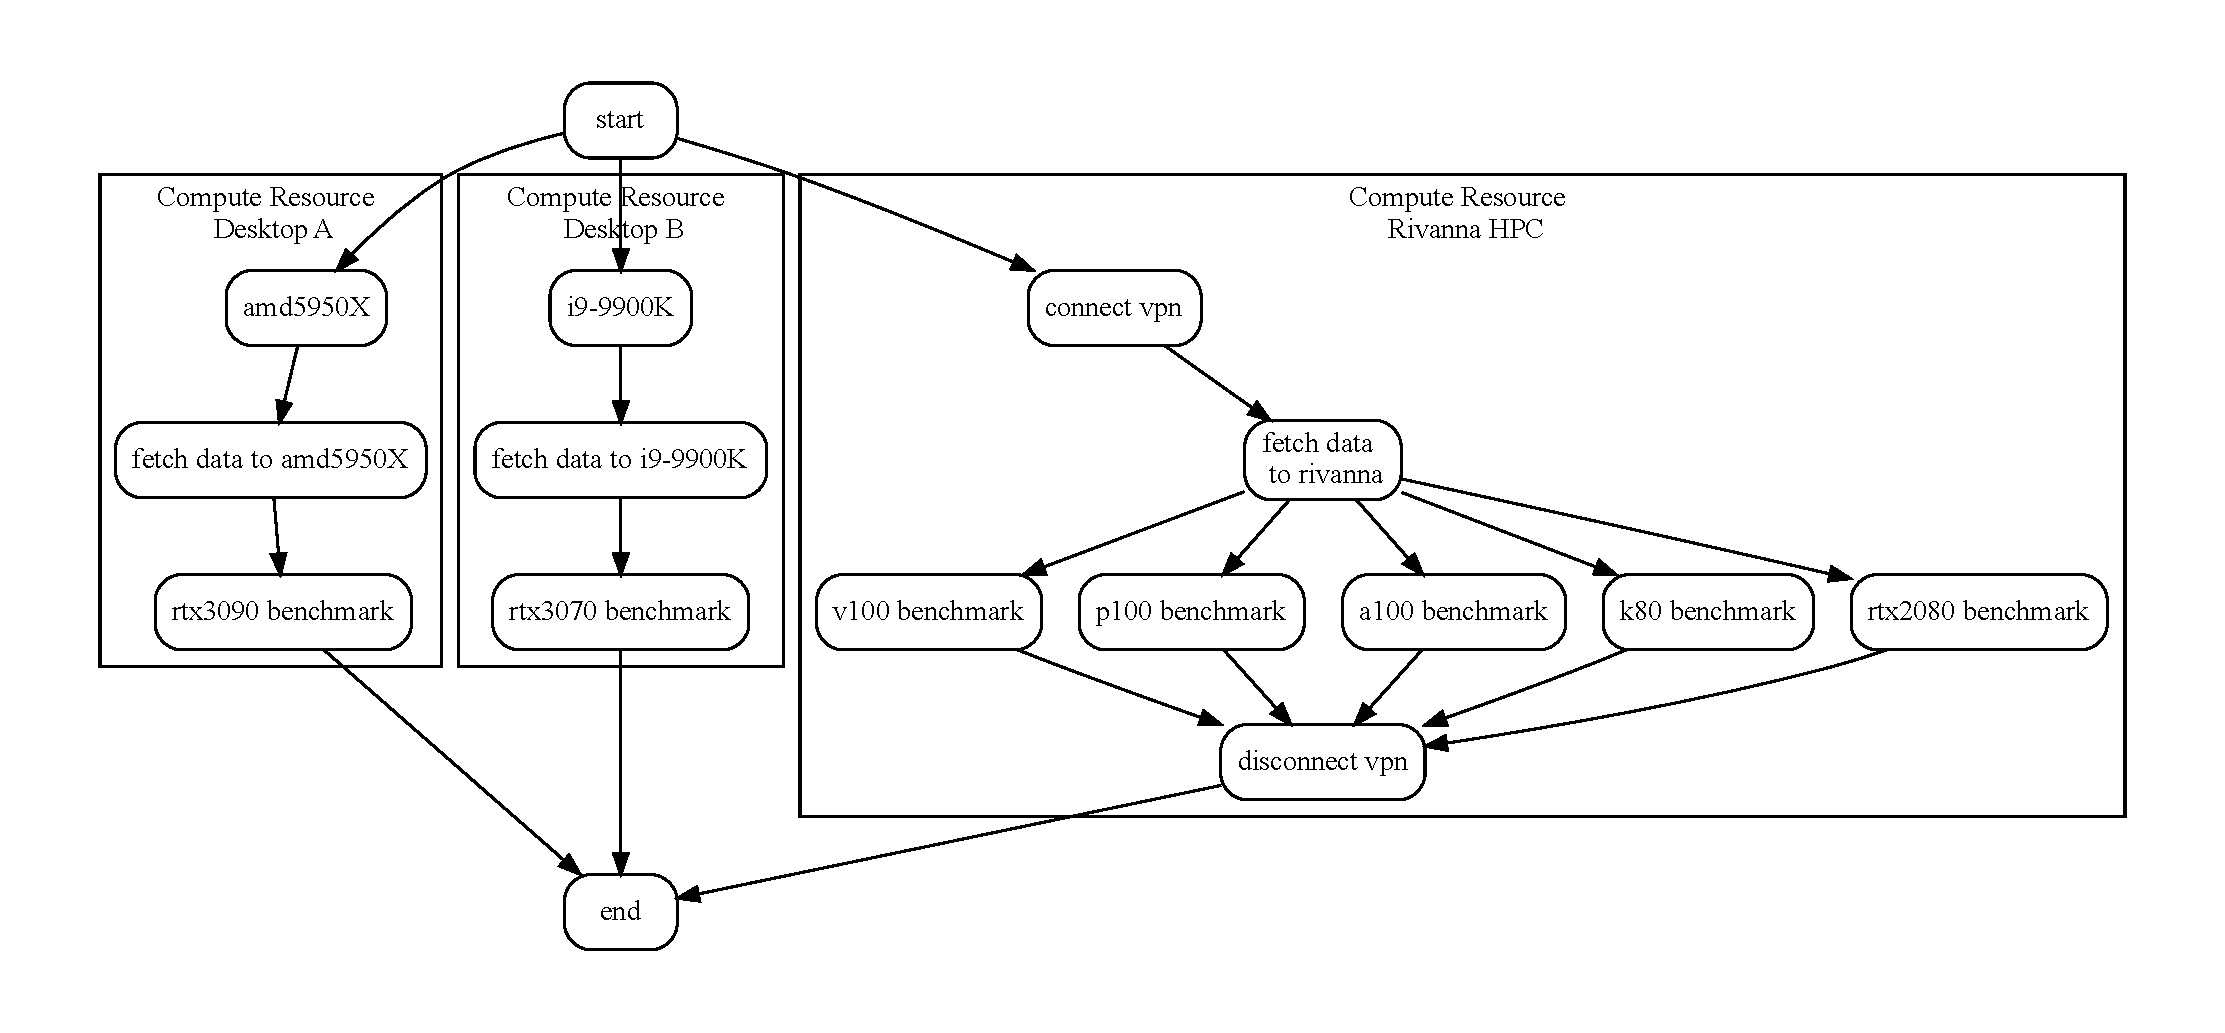
\includegraphics[width=0.75\textwidth]{images/cloudmask-wf.pdf}
%\vspace{-1cm}
\caption{Workflow for Cloudmask}\label{fig:cloudmaskwf}
\end{figure*}

The workflow will take approximately 24 hours to run if resources are
available. The workflow iterates through the five GPUs available on
Rivanna, including V100, P100, A100, K80, and RTX2080, and runs the
program three times on each GPU. Each run trains the model with 10,
30, and 50 epochs for benchmarking. Upon completing a run, the logs
and benchmarks are written into a results folder. In the appendix we
showcase how to run a portion of this workflow while utilizing
only Rivanna (see Appendix~\ref{sec:running-cloudmask}).



%\section{MNIST Workflow}\label{mnist-workflow}

For this example we use UVA's Rivanna machine. Please adopt it to your
HPC machine.

We can test Rivanna's GPUs and benchmark their runtimes for running
several MNIST Python programs. These programs include machine learning
processing, convolutional neural network, long short-term memory,
recurrent neural network, and others. The programs can be found at
\url{https://github.com/cybertraining-dsc/reu2022/tree/main/code/deeplearning/mnist}

To run the MNIST remote workflow on Rivanna, first ensure that your UVA
computing ID is set with the following command:

\begin{verbatim}
cms set username=XXXXXX
\end{verbatim}

where the X's are substituted with your computing ID.

Then, issue commands:

\begin{verbatim}
cd ~/cm/cloudmesh-cc
pytest -v -x --capture=no examples/example_run_mnist_workflow_exec.py
\end{verbatim}

This program uses SLURM and a shell script to iterate through the
available GPUs on Rivanna, which are V100, A100, K80, P100, and RTX2080.

On a successful run, the output will be similar to the following:

\begin{verbatim}
+---------+----------+---------+---------+---------------------+
| Name    | Status   |    Time |     Sum | Start               |
|---------+----------+---------+---------+---------------------+
| v100    | ok       | 138.087 | 138.087 | 2022-09-29 18:15:45 |
| a100    | ok       | 106.046 | 106.046 | 2022-09-29 18:18:05 |
| k80     | ok       | 171.057 | 171.057 | 2022-09-29 18:19:52 |
| p100    | ok       | 202.055 | 202.055 | 2022-09-29 18:22:44 |
| rtx2080 | ok       | 138.048 | 138.048 | 2022-09-29 18:26:07 |
+---------+----------+---------+---------+---------------------+
\end{verbatim}


\FILE{mnist.tex}

\subsection{MNIST Workflow}\label{mnist-workflow}

MNIST is a well-known program to detect handwritten digits. It
provides value for our work because it is well understood and is used
in many educational efforts. Also, we created a workflow that
integrates the UVA Rivanna HPC (the workflow can easily be adapted to other
machines). The nice feature about this application is that it can be
configured to run very quickly while still using various GPUs and
benchmark their runtimes for running several MNIST Python
programs. These programs include machine learning processing,
convolutional neural network, long short-term memory, recurrent neural
network, and others. The programs can be found on
GitHub~\cite{www-mnist-programs}.

As for the workflow, we adapted it not only to run one algorithm but
multiple in an iteration across the GPUs (similar to
\ref{fig:cloudmaskwf}).

On a successful run, the output will be receiving runtimes similar to:

\begin{table}[!ht]
\caption{MNIST Performance as obtained by cloudmesh-cc on various graphics cards using workflow scheduling}
    \centering
    \begin{tabular}{lr}
    \hline
        Name & Time \\ \hline
        a100 & 106.046 \\ 
        v100 & 138.087 \\ 
        rtx2080 & 138.048 \\
        k80 & 171.057 \\ 
        p100 & 202.055 \\
    \end{tabular}
    \label{table:mnist-times}
  \end{table}
  


% \FILE{conclusion.tex}

\section{Conclusion}

TBD

\FILE{conclusion.tex}

\section{Conclusion}

We have designed and implemented a Hybrid Reusable Computational
Analytics Workflow Management with the help of the cloudmesh component
framework. The component added focuses on the management of workflows
for computational analytics tasks and jobs. The tasks can be executed
on remote resources via ssh and even access queuing systems such as
Slurm. In addition, we can integrate the current computer on which the
workflow is running. This can include operating systems such as Linux,
macOS, Windows, and even Windows Subsystem for Linux. Through
cloudmesh, access to a command line and a command shell is provided. A
simple API and a REST interface are provided. The framework also has
an elementary Web browser interface that allows visualizing the
execution of the workflow. It is important to know that the workflow
can be started on remote resources and is running completely
independently from the client tool once a task is started. This allows
a ``stateless'' model that can synchronize with the remotely started
jobs on demand. Hence, the framework is self-recovering in case of
network interruptions or power failure. Due to our experiences with
real (and many) infrastructure failures at the authors' locations, the
availability of such a workflow-guided system was
beneficial. Furthermore, the developed code is rather small and, in
contrast to other systems, is less complex. Hence, it is suitable for
educational aspects as it is used for master's and undergraduate level
research projects. The project has also been practically utilized
while generating benchmarks for the MLCommons Science Working Group
showcasing real-world applicability beyond a student research project.


% \FILE{acknowledgements.tex}

%\begin{ack}

\section*{Acknowledgements}

Continued work was in part funded by the NSF CyberTraining: CIC:
CyberTraining for Students and Technologies from Generation Z with the
award numbers 1829704 and 2200409 and NIST 60NANB21D151T. We like to
thank the students that participated in the REU for their help and
evaluation in a pre-alpha version of the code. We are excited that
this effort contributed significantly to their increased understanding
of Python and how to develop in a team using the Python ecosystem.

%\end{ack}


\FILE{acknowledgements.tex}

%\begin{ack}

\section*{Acknowledgements}

Continued work was in part funded by the NSF CyberTraining: CIC:
CyberTraining for Students and Technologies from Generation Z with the
award numbers 1829704 and 2200409 and NIST 60NANB21D151T. We would like to
thank the students that participated in the REU for their help and
evaluation in a pre-alpha version of the code. We are excited that
this effort contributed significantly to their increased understanding
of Python and how to develop in a team using the Python ecosystem.

%\end{ack}


\bibliographystyle{ACM-Reference-Format}
\bibliography{references,references-cc}



\appendix

\section{Appendix}

% \FILE{installation.tex}

\section{Installation}\label{installation}

To leverage cloudmesh-cc, use the cloudmesh-installer to install the
Cloudmesh suite of repositories. Optionally, to utilize the graph
visualization you must install also {\em graphviz} must be
installed. On Windows, Git Bash is required, in addition.  The overall
installation is very simple and is supported on a variety of operating
systems.  We leverage the cloudmesh-installer to locally install the
cloudmesh suite of repositories by executing the following commands:

\begin{minted}[breaklines]{bash}
$ mkdir ~/cm
$ cd ~/cm
$ pip install cloudmesh-installer -U
$ cloudmesh-installer get cc
\end{minted}

To install graphviz you can use the following commands on the appropriate operating system:

\begin{description}

\item[Windows.]
Git Bash and Graphviz must be installed. The user can use Chocolatey to run
as an administrator for convenience:

\begin{minted}[breaklines]{bash}
$ choco install git.install --params "/GitAndUnixToolsOnPath /Editor:Nano /PseudoConsoleSupport /NoAutoCrlf" -y
$ choco install graphviz -y
\end{minted}

\item[macOS.] Graphviz must be installed. The user can use Homebrew for convenience:

\begin{minted}[breaklines]{bash}
$ brew install graphviz
\end{minted}

\item[Linux.] Graphviz must be installed. The user can use apt for convenience:

\begin{minted}[breaklines]{bash}
$ sudo apt install graphviz -y
\end{minted}

\end{description}

To test the workflow program, prepare a cm directory in your home
directory by executing the following commands:

\begin{minted}[breaklines]{bash}
$ cd ~/cm/cloudmesh-cc
$ pytest -v -x --capture=no tests
\end{minted}

A variety of separate tests are available that test individual capabilities. 


\FILE{installation.tex}

\subsection{Installation}\label{installation}

To leverage cloudmesh-cc, use the cloudmesh-installer to install the
Cloudmesh suite of repositories. Optionally, to utilize the graph
visualization you must install also {\em graphviz} must be
installed. On Windows, Git Bash is required, in addition.  The overall
installation is very simple and is supported on a variety of operating
systems.  We leverage the cloudmesh-installer to locally install the
cloudmesh suite of repositories by executing the following commands:

\begin{minted}[breaklines]{bash}
$ mkdir ~/cm
$ cd ~/cm
$ pip install cloudmesh-installer -U
$ cloudmesh-installer get cc
\end{minted}

To install graphviz you can use the following commands on the
appropriate operating system:

\begin{description}

\item[Windows.]  Git Bash and Graphviz must be installed. The user
can use an instance of Chocolatey that is run as an administrator for
convenience:

\begin{minted}[breaklines]{bash}
$ choco install git.install --params "/GitAndUnixToolsOnPath /Editor:Nano /PseudoConsoleSupport /NoAutoCrlf" -y
$ choco install graphviz -y
\end{minted}

\item[macOS.] Graphviz must be installed. The user can use Homebrew
for convenience:

\begin{minted}[breaklines]{bash}
$ brew install graphviz
\end{minted}

\item[Linux.] Graphviz must be installed. The user can use apt for
convenience:

\begin{minted}[breaklines]{bash}
$ sudo apt install graphviz -y
\end{minted}

\end{description}

To test the workflow program, prepare a cm directory in your home
directory by executing the following commands:

\begin{minted}[breaklines]{bash}
$ cd ~/cm/cloudmesh-cc
$ pytest -v -x --capture=no tests
\end{minted}

A variety of separate tests are available that test individual
capabilities.


% \FILE{cloudmask-appendix.tex}

\subsection{Running Cloudmask Workflow}\label{sec:running-cloudmask}

To run the Cloudmask workflow, run the following commands:

\begin{minted}[breaklines]{bash}
$ cd ~/cm
$ git clone https://github.com/laszewsk/mlcommons.git
$ cd mlcommons
$ pytest -v -x --capture=no benchmarks/cloudmask/target/rivanna/run_cloudmask_workflow.py
\end{minted}


\FILE{cloudmask-appendix.tex}

\subsection{Running Cloudmask Workflow}\label{sec:running-cloudmask}

To run the Cloudmask workflow, run the following commands:

\begin{minted}[breaklines]{bash}
$ cd ~/cm
$ git clone https://github.com/laszewsk/mlcommons.git
$ cd mlcommons
$ pytest -v -x --capture=no benchmarks/cloudmask/target/rivanna/run_cloudmask_workflow.py
\end{minted}


% \section{Contributing}\label{contributing}

\subsection{GitHub}\label{github}

The code is maintained on GitHub

\begin{itemize}
\tightlist
\item
  \href{https://github.com/cloudmesh/cloudmesh-cc}{Code}
\item
  \href{https://github.com/cloudmesh/cloudmesh-cc/issues}{Issues}
\item
  \href{https://github.com/cloudmesh/cloudmesh-cc/pulls}{Pull Requests}
\item
  \href{https://github.com/cloudmesh/cloudmesh-cc/actions}{Actions}
\item
  \href{https://github.com/cloudmesh/cloudmesh-cc/pulse}{Insights}
\end{itemize}

The code was developed by Gregor von Laszewski and J.P. Fleischer. Other
contributors to a pre alpha version are listed at

\begin{itemize}
\tightlist
\item
  \href{https://github.com/cloudmesh/cloudmesh-cc/graphs/contributors}{Contributors}
\end{itemize}

\subsection{Management}\label{management}

All contributions will be done under the apache license. The code will
be managed in open-source. Pull requests need to be made in the
repository. The main branch is the release branch. Contributions will
first be done in other branches, and once we agree that they need to be
integrated into the code, they will be merged into main. All new code
must have sufficient pytests. The pytests may need to be documented in
case special authentication is required.

We follow a
\href{https://docs.github.com/en/get-started/quickstart/github-flow}{typical
GitHub workflow} of:

\begin{itemize}
\tightlist
\item
  create a personal fork of this repo
\item
  create a branch
\item
  open a pull request
\item
  fix findings of various linters and checks
\item
  work through code review
\end{itemize}

For each pull request, the documentation is built and deployed to make
it easier to review the changes in the pull request.

\hypertarget{tests}{%
\subsection{Tests}\label{tests}}

Before creating a pull request it is important that the tests in the
test directory pass.

The tests are organized as follows:

\begin{itemize}
\tightlist
\item
  \texttt{pytest\ tests/test\_0??\_*} will run locally and only use
  ascii output
\item
  \texttt{pytest\ tests/test\_1??\_*} will run locally but also present
  graphs
\end{itemize}

in future we will likely change this and allow a test variable
\texttt{cms\ set\ test\_with\_graph=False/True} and if it is not
existent it is False. In case it is false the graohs will not be
displayed. but the test will be run. This change will also allow tests
with 1?? to be run on github workflows

\begin{itemize}
\tightlist
\item
  \texttt{pytest\ tests/test\_5??\_*} will run on remote machines and
  require at this time rivanna from UVA
\end{itemize}

in future this test will be modified so we can specify the remote user
and remote host \texttt{cms\ set\ test\_remote\_user=TBD}
\texttt{cms\ set\ test\_remote\_host=TBD}. If they do not exist they
will use the defualts from ssh config rivanna. verify if logic is ok.

\begin{itemize}
\tightlist
\item
  \texttt{pytest\ tests/test\_6??\_*} will test the rest service
\item
  \texttt{pytest\ tests/test\_9??\_*} will cleanup the tests
\end{itemize}


\FILE{contributing.tex}

\subsection{Contributing}\label{contributing}

All contributions are done under the Apache License. The code is
maintained as an open-source project on GitHub while using the typical
GitHub code management tools such as:

\begin{itemize}
\item
  \href{https://github.com/cloudmesh/cloudmesh-cc}{Code Repository}
\item
  \href{https://github.com/cloudmesh/cloudmesh-cc/issues}{Issue Management}
\item
  \href{https://github.com/cloudmesh/cloudmesh-cc/pulls}{Pull Request Management}
\item
  \href{https://github.com/cloudmesh/cloudmesh-cc/actions}{Automatic verification with GitHub Actions}
\end{itemize}

The main branch is the release branch and is supposed to be functional
at all times. Hence, contributions are first done in other branches,
and once agreeing that they need to be integrated into the code, they
are merged into main. All new code must be documented and have
sufficient automated tests. Before creating a pull request, it is
important that the tests within the test directory are passing. The
repository already contains several pytests that can be leveraged to
conduct routine testing of the code, including its SSH remote
functionality, REST capability, and Python interface, among others.


\title{Hybrid Reusable Computational Analytics Workflow Management with Cloudmesh}

% \author{Gregor von Laszewski}
\email{laszewski@gmail.com}
\orcid{0000-0001-9558-179X}
\authornote{Corresponding author}
\affiliation{%
  \institution{University of Virginia}
  \streetaddress{Biocomplexity Institute\\
Town Center Four\\
994 Research Park Boulevard}
  \city{Charlottesville}
  \state{VA}
  \postcode{22911}
  \country{USA}
}

\author{J.P. Fleischer}
\orcid{0000-0002-1102-1910}
\affiliation{%
  \institution{University of Virginia}
  \streetaddress{Biocomplexity Institute\\
Town Center Four\\
994 Research Park Boulevard}
  \city{Charlottesville}
  \state{VA}
  \postcode{22911}
  \country{USA}
}

\author{Geoffrey C. Fox}
\email{gcfexchange@gmail.com}
\affiliation{%
  \institution{University of Virginia}
  \streetaddress{Biocomplexity Institute\\
Town Center Four\\
994 Research Park Boulevard}
  \city{Charlottesville}
  \state{VA}
  \postcode{22911}
  \country{USA}
}

\author{Wo L. Chang}
\email{wchang@nist.gov}
\affiliation{%
  \institution{NIST}
  \streetaddress{Information Technology Laboratory\\
100 Bureau Drive}
  \city{Gaithersburg}
  \state{MD}
  \postcode{20899}
  \country{USA}
}

\renewcommand{\shortauthors}{von Laszewski, et al.}


\author{Gregor von Laszewski}
\email{laszewski@gmail.com}
\orcid{0000-0001-9558-179X}
\authornote{Corresponding author}
\affiliation{%
  \institution{University of Virginia}
  \streetaddress{Biocomplexity Institute\\
Town Center Four\\
994 Research Park Boulevard}
  \city{Charlottesville}
  \state{VA}
  \postcode{22911}
  \country{USA}
}

\author{J.P. Fleischer}
\email{jacquespfleischer@gmail.com}
\orcid{0000-0002-1102-1910}
\affiliation{%
  \institution{University of Virginia}
  \streetaddress{Biocomplexity Institute\\
Town Center Four\\
994 Research Park Boulevard}
  \city{Charlottesville}
  \state{VA}
  \postcode{22911}
  \country{USA}
}

\author{Geoffrey C. Fox}
\email{gcfexchange@gmail.com}
\orcid{0000-0003-1017-1391}
\affiliation{%
  \institution{University of Virginia}
  \streetaddress{Biocomplexity Institute\\
Town Center Four\\
994 Research Park Boulevard}
  \city{Charlottesville}
  \state{VA}
  \postcode{22911}
  \country{USA}
}

\begin{comment}
\author{Wo L. Chang}
\email{wchang@nist.gov}
\affiliation{%
  \institution{NIST}
  \streetaddress{Information Technology Laboratory\\
100 Bureau Drive}
  \city{Gaithersburg}
  \state{MD}
  \postcode{20899}
  \country{USA}
}
\end{comment}

\renewcommand{\shortauthors}{von Laszewski, et al.}

\begin{abstract}

% \FILE{abstract.tex}

In this paper, we summarize our effort to create and utilize a {\em simple} framework to coordinate computational analytics tasks with the help of a workflow system. Our design is based on a minimalistic approach while at the same time allowing to access computational resources offered through the owner's computer, HPC computing centers, cloud resources, and distributed systems in general. The access to this framework includes a simple GUI for monitoring and managing the workflow, a REST service, a command line interface, as well as a Python interface. The resulting framework was developed for several examples targeting benchmarks of AI applications on hybrid compute resources and as an educational tool for teaching scientists and students sophisticated concepts to execute computations on resources ranging from a single computer to many thousands of computers as part of on-premise and cloud infrastructure. We demonstrate the usefulness of the tool on a number of examples. The code is available as an open-source project in GitHub and is based on an easy-to-enhance tool called cloudmesh.

 \FILE{abstract.tex}

 In this paper, we summarize our effort to create and utilize a {\em
 simple} framework to coordinate computational analytics tasks with
 the help of a workflow system. Our design is based on a minimalistic
 approach while at the same time allowing to access computational
 resources offered through the owner's computer, HPC computing
 centers, cloud resources, and distributed systems in general. The
 access to this framework includes a simple GUI for monitoring and
 managing the workflow, a REST service, a command line interface, as
 well as a Python interface. The resulting framework was developed for
 several examples targeting benchmarks of AI applications on hybrid
 compute resources and as an educational tool for teaching scientists
 and students sophisticated concepts to execute computations on
 resources ranging from a single computer to many thousands of
 computers as part of on-premise and cloud infrastructure. We
 demonstrate the usefulness of the tool on a number of examples. The
 code is available as an open-source project in GitHub and is based on
 an easy-to-enhance tool called cloudmesh.
 
\end{abstract}


% 
\begin{CCSXML}
<ccs2012>
<concept>
<concept_id>10010520.10010521.10010537</concept_id>
<concept_desc>Computer systems organization~Distributed architectures</concept_desc>
<concept_significance>500</concept_significance>
</concept>
<concept>
<concept_id>10010520.10010521.10010537.10003100</concept_id>
<concept_desc>Computer systems organization~Cloud computing</concept_desc>
<concept_significance>500</concept_significance>
</concept>
<concept>
<concept_id>10011007.10010940.10010971.10011120</concept_id>
<concept_desc>Software and its engineering~Distributed systems organizing principles</concept_desc>
<concept_significance>500</concept_significance>
</concept>
</ccs2012>
\end{CCSXML}

\ccsdesc[500]{Computer systems organization~Distributed architectures}
\ccsdesc[500]{Computer systems organization~Cloud computing}
\ccsdesc[500]{Software and its engineering~Distributed systems organizing principles}

\keywords{high performance computing, batch queue, service}




\begin{CCSXML}
<ccs2012>
<concept>
<concept_id>10010520.10010521.10010537</concept_id>
<concept_desc>Computer systems organization~Distributed architectures</concept_desc>
<concept_significance>500</concept_significance>
</concept>
<concept>
<concept_id>10010520.10010521.10010537.10003100</concept_id>
<concept_desc>Computer systems organization~Cloud computing</concept_desc>
<concept_significance>500</concept_significance>
</concept>
<concept>
<concept_id>10011007.10010940.10010971.10011120</concept_id>
<concept_desc>Software and its engineering~Distributed systems organizing principles</concept_desc>
<concept_significance>500</concept_significance>
</concept>
</ccs2012>
\end{CCSXML}

\ccsdesc[500]{Computer systems organization~Distributed architectures}
\ccsdesc[500]{Computer systems organization~Cloud computing}
\ccsdesc[500]{Software and its engineering~Distributed systems organizing principles}

\keywords{high performance computing, batch queue, service}



%\received{20 February 2007}
%\received[revised]{12 March 2009}
%\received[accepted]{5 June 2009}

% set page numbers
\settopmatter{printfolios=true}

\maketitle

% \FILE{cc.tex}

\section{Introduction}

In this section we provide an introduction to or work while 
moving forward to motivate a 
Hybrid Reusable Computational Analytics Workflow
Management Framework.

\subsection{Reusable Computational Analytics}

{\em Reusable computational analytics} (RCA) focuses on  the creation of reusable programs, patterns, and services to conduct analytics tasks that are part of the scientific discovery process.  RCA service need varies widely and may include multi-scale hardware resources as well as multi-scale scientific applications. To utilize such services and their resources in a reusable way we need to have a mechanism to express them in an easy fashion that goes beyond just the definition in one programming language or framework, but allows the integration into many different programming languages and frameworks so that services that may be designed in one framework or language may be reusable in others.

\subsection{Reusable Multi-scale Algorithms}

In current scientific problems we encounter a rich set of applications that leverage a number of sophisticated methods that may require adaptations on multiple scales. The scales are influenced by their Domain size, accuracy and time requirement to solve them in sufficient manner. It is of advantage to provide reusable components that can be controlled by parameters to simplify reuse.

\subsection{Hybrid Cloud and Compute Resources and Serices}

As we deal with multi-scale algorithms not every analytics task needs to be conducted on a High Performance Computer (HPC). This is especially the case with the advent of GPUs in the desktop which we termed in the authors termed in past with {\em desktop supercomputing}. Also the availability of cloud computers and hyper-scale data centers play a significant role in today's analytics processes. This not only includes the use compute resources, but also services that are these days offered by cloud service providers. A well known example for this is natural language processing.

\subsection{Reusable and Adaptable HPC and Cloud Service Workflows}

High-performance computing (HPC) has been, for decades, a very important tool
for science. Scientific tasks can leverage the processing power of
a supercomputer so they can run at previously unobtainable high speeds
or utilize specialized hardware for acceleration that otherwise are not
available to the user. HPC can be used for analytic programs that
leverage machine learning applied to large data sets to, for example,
predict future values or to model current states. For such
high-complexity projects, there are often multiple complex programs that
may be running repeatedly in either competition or cooperation.
Leveraging computational GPUs, for instance, leads to several times higher
performance when applied to deep learning algorithms. With such
projects, program execution is submitted as a job to a typically remote
HPC center, where time is billed as node hours. Such projects must have
a service that lets the user manage and execute without supervision. We
have created a service that lets the user run jobs across multiple
platforms in a dynamic queue with visualization and data storage.

Similar aspects are available for cloud services that abstract the infrastructure needs and focus on the availability of services that can be integrated in concert with HPC, as well as the users local resources (for example a PC).




\FILE{cc.tex}

\section{Introduction}

In this section we provide an introduction to our work while
moving forward to motivate a 
Hybrid Reusable Computational Analytics Workflow
Management Framework.

\subsection{Reusable Computational Analytics}

{\em Reusable computational analytics} (RCA) focuses on the creation
of reusable programs, patterns, and services to conduct analytics
tasks that are part of the scientific discovery process. RCA service
need varies widely and may include multi-scale hardware resources as
well as multi-scale scientific applications. To utilize such services
and their resources in a reusable way, we need to have a mechanism to
express them in an easy fashion that goes beyond just the definition
in one programming language or framework, but allows the integration
into many different programming languages and frameworks so that
services that may be designed in one framework or language may be
reusable in others.

\subsection{Reusable Multi-scale Algorithms}

In current scientific problems we encounter a rich set of applications
that leverage a number of sophisticated methods that may require
adaptations on multiple scales. The scales are influenced by their
Domain size, accuracy and time requirement to solve them in a
sufficient manner. It is of advantage to provide reusable components
that can be controlled by parameters to simplify reuse.

\subsection{Hybrid Cloud and Compute Resources and Serices}

As we deal with multi-scale algorithms, not every analytics task needs
to be conducted on a High Performance Computer (HPC). This is
especially the case with the advent of desktop GPUs, which authors
have termed in past {\em desktop supercomputing}. Also the
availability of cloud computers and hyper-scale data centers play a
significant role in today's analytics processes. This not only
includes the use compute resources, but also services that are these
days offered by cloud service providers. A well-known example for this
is natural language processing.

\subsection{Reusable and Adaptable HPC and Cloud Service Workflows}

High-performance computing (HPC) has been, for decades, a very important tool
for science. Scientific tasks can leverage the processing power of
a supercomputer so they can run at previously unobtainable high speeds
or utilize specialized hardware for acceleration that otherwise are not
available to the user. HPC can be used for analytic programs that
leverage machine learning applied to large data sets to, for example,
predict future values or to model current states. For such
high-complexity projects, there are often multiple complex programs that
may be running repeatedly in either competition or cooperation.
Leveraging computational GPUs, for instance, leads to several times higher
performance when applied to deep learning algorithms. With such
projects, program execution is submitted as a job to a typically remote
HPC center, where time is billed as node hours. Such projects must have
a service that lets the user manage and execute without supervision. We
have created a service that lets the user run jobs across multiple
platforms in a dynamic queue with visualization and data storage.

Similar aspects are available for cloud services that abstract the
infrastructure needs and focus on the availability of services that
can be integrated in concert with HPC, as well as the users local
resources (for example a PC).




% \FILE{requirements.tex}

\section{Requirements}

For the design of the framework we have the following requirements.

\begin{description}

\item[Simplicity.] The design must e simpla and the code base must be small. THis helps the future maintenance of the code, but also allows the code to become part of eductaional oppertunities such as in Research experience for undergraduates (REU), capstone project, and class projects. The challange here is that many other systems are too big to be used in introductory undergraduate and mastares activities. 
However the framework should be capable enough to support also research projects.

\item[Workflow specification.]  The specification of the workflow must be simple. From the past we have learned that the introduction of programming controll components such as loops, and conditions, in addition to DAG's is essential to provide maximum flexibility. 

\item[Workflow Monitoring.] The workflow framework must be able to monitor the progress of individual jobs as well as the overall progress of the workflow. 

\item[Workflow Interfaces.] To specify and interface with the workflow we must provide several interface layers. This includes, specification through a YAML file, interfacing  through REST calles, interfacing through a python API, and interfaceing with a very simple GUI component. For the workflow monitoring with the GUI we must be able to easily define custom text to reflect user designable monitoring labels.

\item[Langaugae Independence.] As we want to make the framework integratable in other frameworks we need a simple mechanism to provide either API or interface portability. To keep the code base small a REST API seems very well suited.

\item[OpenAPI.] To further strengthen usability the framework must have an OpenAPI interface. THis allows the integration via 3rd party tools into other frameworks and languages if desired.

\item[Hybrid multicloud Providers.] The service must be able to be deployable on an on-premisse local computer or various cloud providers.

\item[Generalized Job Interface.] The framework must be able to interface 
with a wide variety of computation services. This includes the support
of ssh, batch queues such as SLURM and LSF, local compute resources
including shell scripts as well as support for WSL.

\item[Support of various Operating Systems.] The framework must be runnable on various client operating systems including Linux, macOS, Windows.

\item[State Management.] The state management must be recoverable and the client must be able to completely recover from a network failure. As such the state will be queried on demand. This allows one to deploy the framework on a laptop, start the workflow, close or shutdown the laptop and at a alater time open the laptop while the workflow framework can be refreshed with the latest state.

\end{description}


\FILE{requirements.tex}

\section{Requirements}

For the design of the framework, we have the following requirements.

\begin{description}

\item[Simplicity.] The design must be simple and the code base must be
small.  This helps the future maintenance of the code, but also allows
the code to become part of educational opportunities such as in a
Research Experience for Undergraduates (REU), capstone project, and
class projects. The challenge here is that many other systems are too
big to be used in introductory undergraduate and masters activities.
However, the framework should be capable enough to also support
research projects.

\item[Workflow specification.] The specification of the workflow must
be simple.  From the past we have learned that the introduction of
programming control components such as loops, and conditions, in
addition to DAGs, is essential to provide maximum flexibility.

\item[Workflow Monitoring.] The workflow framework must be able to
monitor the progress of individual jobs as well as the overall
progress of the workflow.

\item[Workflow Interfaces.] To specify and interface with the
workflow, we must provide several interface layers. This includes
specification through a YAML file, interfacing through REST calls,
interfacing through a Python API, and interfacing with a very simple
GUI component.  For the workflow monitoring with the GUI, we must be
able to easily define custom text to reflect user designable
monitoring labels.

\item[Language Independence.] As we want to make the framework
integrable in other frameworks, we need a simple mechanism to provide
either API or interface portability. To keep the code base small, a
REST API seems very well-suited.

\item[OpenAPI.] To further strengthen usability, the framework must
have an OpenAPI interface. This allows the integration via 3rd party
tools into other frameworks and languages, if desired.

\item[Hybrid multicloud Providers.] The service must be able to be
deployable on an on-premise local computer or various cloud providers.

\item[Generalized Job Interface.] The framework must be able to
interface with a wide variety of computation services. This includes
the support of ssh, batch queues such as Slurm and LSF, and local
compute resources including shell scripts, as well as support for WSL.

\item[Support of various Operating Systems.] The framework must be
runnable on various client operating systems including Linux, macOS,
Windows.

\item[State Management.] The state management must be recoverable and
the client must be able to completely recover from a network failure.
As such, the state will be queried on demand. This allows one to
deploy the framework on a laptop, start the workflow, close or
shutdown the laptop, and at a later time open the laptop while the
workflow framework can be refreshed with the latest state.

\end{description}

% \FILE{related-research.tex}

\section{Related Research}

Many different workflow systems have been developed in the past.  It
is out of scope of this document to present a complete overview of all
the different stystems. Instead we compare some selected features of
the systems and identify features that are important for us. The
following features are important.

\begin{description}

\item[Batch.] Long running jobs on HPC systems are coordinated through Batch services.

\item[Resource Reservation.] In some cases access to batch queuses on HPC systems take a long time in case of many different tasks it is sometimes useful to researce a number of batch nodes and run many short running programs on them if the need arises. THis haowever can often be replacesd just with properly coordinated workflows using a batch system. In fact frameworks using such reservation internally implement them using the batch system.

\item[Computational Grids.] Grids provide a service level access to distributed HPC computing resources. However Grids popular a decade ago are no longer the predominantly deployed and focus has shifted to CLoud computing. 

\item[Cloud.] Computing resourcesa are these days also available in the cloud as HPC, batch, and compute services, including specialized SaaS offerings that allow to integrate analytics finctions into workflows.

\item[REST.] The predominant specification for cloud services uses the REST framework relying on a stateles model. This contrasts the WSRF model that uses statefull services.

\item[Specification.] Some work has focused on the spcification of the workflows rather.

\item[GUI.] Some foremworks provide extensive GUIs.

\end{description}

In Table \ref{tab:workflow-table} we provide a number of examples for the various
features we found in workflow systems.


\begin{table*}[htb]

\caption{Example of workflow frameworks with selected features.}
\label{tab:workflow-table}q

\resizebox{1.0\textwidth}{!}{
{\footnotesize
\begin{tabular}{|p{3cm}|p{3cm}|p{10cm}|}
\hline
{\bf Name} & {\bf Selected Features} & {\bf Description} \\
\hline
\hline

LSF \cite{www-lsf} & Batch, HPC & Batch Queue Manager. \\
\hline

SLURM \cite{www-slurm} & Batch, HPC & Batch queue workflow manager. \\
\hline

Cloudmesh  \cite{www-cloudmesh-manual} & HPC, Cloud, on-Premisse & Suite 
of Python code for cloud computing. \\
\hline

Airflow \cite{www-airflow} & HPC, Cloud, Remote Tasks & ``Airflow is a platform created by the community to programmatically author, schedule and monitor workflows.'' \\
\hline


Loosely coupled Metacomputer \cite{las-1996-thesis,las-1999-loosely} &
                                                                       HPC, on-Premisse
             & Early work on workflow management system comnnecting multiple super computers. \\
\hline

Karajan CoGkit  \cite{las07-workflow} & Service, Langauage, HPC, on-Premisse & Sophisticated Workflow management system with Dag and loops for Grid computing and loosely coupled compute resources thorugh services. \\
\hline

Snakemake  \cite{www-snakemake} & Language & ``The Snakemake workflow management system is a tool to create reproducible and scalable data analyses. Workflows are described via a human readable, Python based language. They can be seamlessly scaled to server, cluster, grid and cloud environments, without the need to modify the workflow definition. Finally, Snakemake workflows can entail a description of required software, which will be automatically deployed to any execution environment.'' \\
\hline

Gridant  \cite{las-2004-gridant} & Language & 
Client based workflow management toolkit to orchestrate complex workflows on the fly without substantial help from the service providers. It integrates on premisse and Grid resources. \\
\hline

Keppler  \cite{www-kepler} & Service, GUI & ``Kepler is designed to help scientists, analysts, and computer programmers create, execute, and share models and analyses across a broad range of scientific and engineering disciplines.'' \\
\hline

Pegasus  \cite{www-pegasus} & DAG, Service, HPC, Coud &  A DAG based workflow management tool for scientific workflow.  \\
\hline

Swift \cite{las-2007-swift} & Language, Many task & A language for distributed parallel scripting.\\
\hline

Parsl \cite{www-parsl} & Language, Many task & A language for distributed parallel scripting. \\
\hline

Radical Pilot \cite{arxiv-radical-pilot} & Many task & Pilot system that enables scalable workflows \\ 
\hline

Gcloud workflow \cite{www-gcloud} & Cloud & Google Cloud documentation for creating a workflow with the command line interface. \\
\hline

Azure REST \cite{www-azure-rest} & Cloud & Microsoft Azure REST API documentation to interface with Azure Logic Apps. \\
\hline

GitHub REST Cancel a Workflow Run \cite{www-github-rest-cancel}
& GitHub Actions
& GitHub REST API documentation to cancel a GitHub Workflow. \\
\hline

ArcGIS Rest \cite{www-arcgis-rest} & & ArcGIS documentation for its REST API to interface with the ArcGIS Server. \\
\hline

Azure Enterprise Workflow \cite{www-azure-enterprise-workflow} & & Article showcasing how to use Enterprise Workflows with Azure Logic Apps. \\
\hline

WSDL \cite{www-wsdl} & Specification & Microsoft Azure schema reference for the Workflow Definition Language in Azure Logic Apps. \\
  \hline

  WSRF \cite{www-wsrf} & Specification & OASIS Web Services Resource Framework\\

AWS Workflow \cite{www-aws-workflow} & & Amazon Web Services documentation definition of a workflow.\\
\hline

AWS SWF \cite{www-aws-swf} & & Amazon Web Services documentation for managing simple workflows with tasks. \\
\hline

AWS Step Functions \cite{www-aws-stepfunctions} & & Amazon Web Services documentation for visual workflow service. \\
\hline

AWS HPC  \cite{www-aws-batch-workflow} & Cloud, HPC & Amazon Web Services documentation for setting workflow dependencies using batch processing in HPC on the cloud. \\
\hline

Azure Batch \cite{www-azure-batch} & Cloud, Batch & Microsoft Azure documentation for running batch service workflows. \\
  \hline

 Business Automation with REST \cite{www-business-rest-ibm} & Buisiness
                                        Process& IBM REST API documentation for its Business Automation Workflows. \\
\hline

  
% --  Artifact Visualization \cite{www-artifact} & & Argo Workflows documentation for kubernetes which shows how to visualize artifacts. \\
% \hline

% -- REST Capabilities for RESTful Workflows \cite{www-rest-workflows} & & Article that demonstrates various examples of REST APIs, such as KNIME. \\
% \hline

Infogram \cite{las-02-infogram} & Service & A Peer-to-Peer Information and Job Submission Service.\\
\hline
\end{tabular}
}
}
\end{table*}


\FILE{related-research.tex}

\section{Related Research}

Many different workflow systems have been developed in the past. It is
out of the scope of this document to present a complete overview of
all the different systems. Instead, we compare some selected features
of the systems and identify features that are important for us. The
following features are important.

\begin{description}

\item[Batch paralelism.] Long-running jobs on HPC systems are coordinated through
Batch services.

\item[Task paralleleism.] Tasks are a logical unit of work that is
executed by a resource, service, or component. Often trask paralelism
is used in distributed resource frameworks.  

\item[Resource Reservation.] In some cases, access to batch queues on
HPC systems take a long time. In the case of many different tasks, it
is sometimes useful to research a number of batch nodes and run many
short-running programs on them if the need arises. This, however, can
often be replaced just with properly coordinated workflows using a
batch system. In fact, frameworks using such reservations internally
implement them using the batch system.

\item[Computational Grids.] Grids provide service-level access to
distributed HPC computing resources. However, Grids (popular a decade
ago) are no longer predominantly deployed and the focus has shifted to
Cloud computing.

\item[Cloud.] Presently, computing resources are also available in
the cloud as HPC, batch, and compute services, including specialized
SaaS offerings that allow to integrate analytics functions into
workflows.

\item[REST.] The predominant specification for cloud services uses the
REST framework relying on a stateless model. This contrasts with the
WSRF model that uses stateful services.

\item[Specification.] Some work has also focused on the specification
of the workflows.

\item[GUI.] Some frameworks provide extensive GUIs.


\end{description}

In Table~\ref{tab:workflow-table}, we provide a number of examples for
the various features we found in workflow systems.


\begin{table*}[htb]

\caption{Example of workflow frameworks with selected features.}
\label{tab:workflow-table}

\resizebox{1.0\textwidth}{!}{
{\footnotesize
\begin{tabular}{|p{3cm}|p{3cm}|p{10cm}|}
\hline
{\bf Name} & {\bf Selected Features} & {\bf Description} \\
\hline
\hline

LSF \cite{www-lsf} & Batch, HPC & Batch Queue Manager. \\
\hline

SLURM \cite{www-slurm} & Batch, HPC & Batch queue workflow manager. \\
\hline

Cloudmesh  \cite{www-cloudmesh-manual} & HPC, Cloud, on-Premise, Task & Suite
of Python code for cloud computing. \\
\hline

Airflow \cite{www-airflow} & HPC, Cloud, Remote Tasks & ``Airflow is a platform created by the community to programmatically author, schedule, and monitor workflows.'' \\
\hline


Loosely coupled Metacomputer \cite{las-1996-thesis,las-1999-loosely} &
                                                                       HPC, on-Premise
             & Early work on workflow management system connecting multiple supercomputers. \\
\hline

Karajan CoGkit  \cite{las07-workflow} & Service, Language, HPC, on-Premise & Sophisticated Workflow management system with Dag and loops for Grid computing and loosely coupled compute resources through services. \\
\hline

Snakemake  \cite{www-snakemake} & Language & ``The Snakemake workflow management system is a tool to create reproducible and scalable data analyses. Workflows are described via a human-readable, Python-based language. They can be seamlessly scaled to server, cluster, grid, and cloud environments, without the need to modify the workflow definition. Finally, Snakemake workflows can entail a description of the required software, which will be automatically deployed to any execution environment.'' \\
\hline

Gridant  \cite{las-2004-gridant} & Language & 
Client-based workflow management toolkit to orchestrate complex workflows on the fly without substantial help from the service providers. It integrates on premise and Grid resources. \\
\hline

Keppler  \cite{www-kepler} & Service, GUI & ``Kepler is designed to help scientists, analysts, and computer programmers create, execute, and share models and analyses across a broad range of scientific and engineering disciplines.'' \\
\hline

Pegasus  \cite{www-pegasus} & DAG, Service, HPC, Cloud &  A DAG-based workflow management tool for scientific workflow.  \\
\hline

Swift \cite{las-2007-swift} & Language, Resource Reservation & A language for distributed parallel scripting.\\
\hline

Parsl \cite{www-parsl} & Language, Resource Reservation & A language for distributed parallel scripting. \\
\hline

Radical Pilot \cite{arxiv-radical-pilot} & Resource Reservation & Pilot system that enables scalable workflows \\ 
\hline

Gcloud workflow \cite{www-gcloud} & Cloud & Google Cloud documentation for creating a workflow with the command line interface. \\
\hline

Azure REST \cite{www-azure-rest} & Cloud & Microsoft Azure REST API documentation to interface with Azure Logic Apps. \\
\hline

GitHub REST Cancel a Workflow Run \cite{www-github-rest-cancel}
& GitHub Actions
& GitHub REST API documentation to cancel a GitHub Workflow. \\
\hline

%ArcGIS Rest \cite{www-arcgis-rest} & & ArcGIS documentation for its REST API to interface with the ArcGIS Server. \\
%\hline

Azure Enterprise Workflow \cite{www-azure-enterprise-workflow} & GUI,
Workflow & Enterprise Workflows with Azure Logic Applications \\
\hline

WSDL \cite{www-wsdl} & Specification & Microsoft Azure schema reference for the Workflow Definition Language in Azure Logic Apps. \\
  \hline

  WSRF \cite{www-wsrf} & Specification & OASIS Web Services Resource Framework\\

AWS Workflow \cite{www-aws-workflow} &  & Amazon Web Services documentation definition of a workflow.\\
\hline

AWS SWF \cite{www-aws-swf} & Task & Amazon Web Services documentation for managing simple workflows with tasks. \\
\hline

AWS Step Functions \cite{www-aws-stepfunctions} & GUI, Task & Amazon Web Services documentation for visual workflow service. \\
\hline

AWS HPC  \cite{www-aws-batch-workflow} & Cloud, HPC & Amazon Web Services documentation for setting workflow dependencies using batch processing in HPC on the cloud. \\
\hline

Azure Batch \cite{www-azure-batch} & Cloud, Batch & Microsoft Azure documentation for running batch service workflows. \\
  \hline

 Business Automation with REST \cite{www-business-rest-ibm} & Business
                                        Process& IBM REST API documentation for its Business Automation Workflows. \\
\hline

  
% --  Artifact Visualization \cite{www-artifact} & & Argo Workflows documentation for Kubernetes which shows how to visualize artifacts. \\
% \hline

% -- REST Capabilities for RESTful Workflows \cite{www-rest-workflows} & & Article that demonstrates various examples of REST APIs, such as KNIME. \\
% \hline

Infogram \cite{las-02-infogram} & Service & A Peer-to-Peer Information and Job Submission Service.\\
\hline
\end{tabular}
}
}
\end{table*}

% \FILE{cc-design.tex}

\section{Design}

To fulfill our requirements we have developed a framework for workflow
controlled computing called Cloudmesh compute cluster that we call
{\em Cloudmesh-cc}. The architecture of the framework is depicted in
Figure~\ref{fig:arch}.

\begin{figure}[htb]
\centering
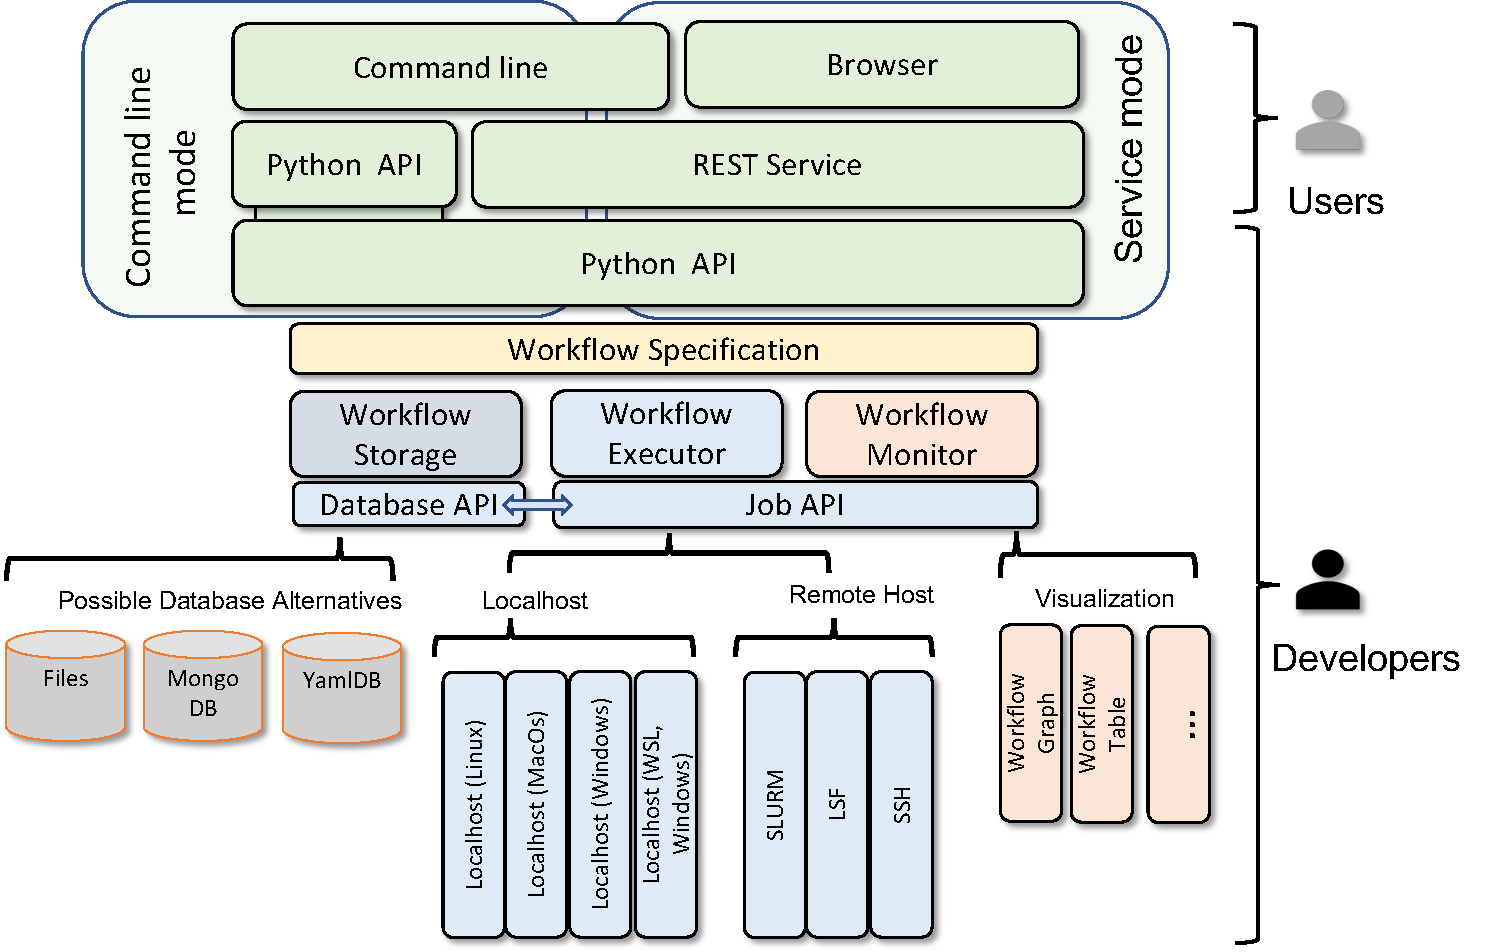
\includegraphics[width=1.0\columnwidth]{images/cloudmesh-cc-arch.pdf}
\caption{Architecture of the Cloudmesh-cc Framework.}\label{fig:arch}
\end{figure}

The framework is based on a layered architecture so it can be improved
and expanded on at each layer. We distinguish two kinds of users,
developers and endusers that define their own workflows to run on
compute resources. For the end user we provide a commandline and a
very simple browser interface. The simplicity is important as it does
not require to spend exorbitant amounts of time to learn how to use
the workflow framework. To support developers we have designed a
minimal Python API that is also used to implement a REST Service.
Currently the REST service is supposed to run on the client, but a
service deployment could also be conducted while assuring that proper
authentication and authorization is used. This is easily possible as
we use a well-known REST service framework (FastAPI) that can integrate
with common security frameworks to secure services. The API, workflow
specification, commandline interface, and browser are well documented
with the help of Sphinx and OpenAPI.

The workflow specification plays an important role to not only define
a workflow, but also to keep the status of a currently executed
workflow. Here we have completely separated the status of the workflow
and synchronize the state of the Workflow with pull requests to the
service that executes the computation. This allows the system to be
shut down at any time while the running jobs are completely
independent from the client application accessing the state. Thus the
client appears to be stateless and fetches the state of the submitted
jobs on demand. It will return the latest state found on the job
execution services.

The workflows are defined with YAML. The workflow is stored in a
database that can be implemented using a variety of backends such as
YamlDB which is file based, MongoDB, or pickle. In our current
implementation we just use a file-based implementation as it does not
require to set up and manage more complex databases. This is an
important capability as we found that scientists and beginning
students do not want to engage in the hassle of setting up and
managing a datastore such as MongoDB.

As we use a YAML file to represent the status of the workflow it is
easy to create monitoring components for example as part of a Web
browser. Various graph sophisticated display frameworks could be
used. For now we have simply exposed the graph in table format using
datatables.net and the graph as SVG while leveraging Graphviz.

One of the most important parts of the framework is how we manage jobs
and monitor their status. For this, we have introduced a abstract job
class that is integrated in our workflow class. The job class has the
ability to define jobs, start them, and cancel them, to name only the
most important management methods. However, each job defines a status
file in which the actual progress of the job is recorded. This status
file is managed on the compute resource where the job is run and is
queried on demand to return the status to the client. This way, the
status of all jobs can be monitored. As our goal is not to run jobs
that execute in milliseconds, but rather than in the second range such
status reporting and propagation is well suited for us. We have
defined a special status progress update specification that is
universally applicable. These jobs can be bash scripts, Python scripts,
Jupyter notebooks, or Slurm scripts.

Workflows are compilations of jobs to be run on nodes. These workflows
report information on the status of jobs as they are run, whether
locally or remotely.  These types of jobs can be mixed
with one another in a single workflow. This allows us, as already mentioned, 
to view the progress of a workflow as it is being run in quasi-realtime.
The workflow can be monitored as a graph or a datatable. These interfaces
report the statuses of the jobs. Additionally, the order in which the jobs
are run can be specified, enabling prerequisite jobs and the segmentation of a
workflow.

To address the requirement of simplicity the overall code is less than
3600 lines of code with additional 2600 lines for extensive test
cases.

The framework is managed as OpenSource repository in GitHub and uses
Python as the implementation language. The code is compatible with
Windows, macOS, and Linux.


\FILE{cc-design.tex}


\section{Design}

To fulfill our requirements, we have developed a framework for
workflow-controlled computing called Cloudmesh compute cluster,
otherwise referred to as {\em Cloudmesh-cc}. The architecture of the
framework is depicted in Figure~\ref{fig:arch}.

\begin{figure}[htb]
{\centering
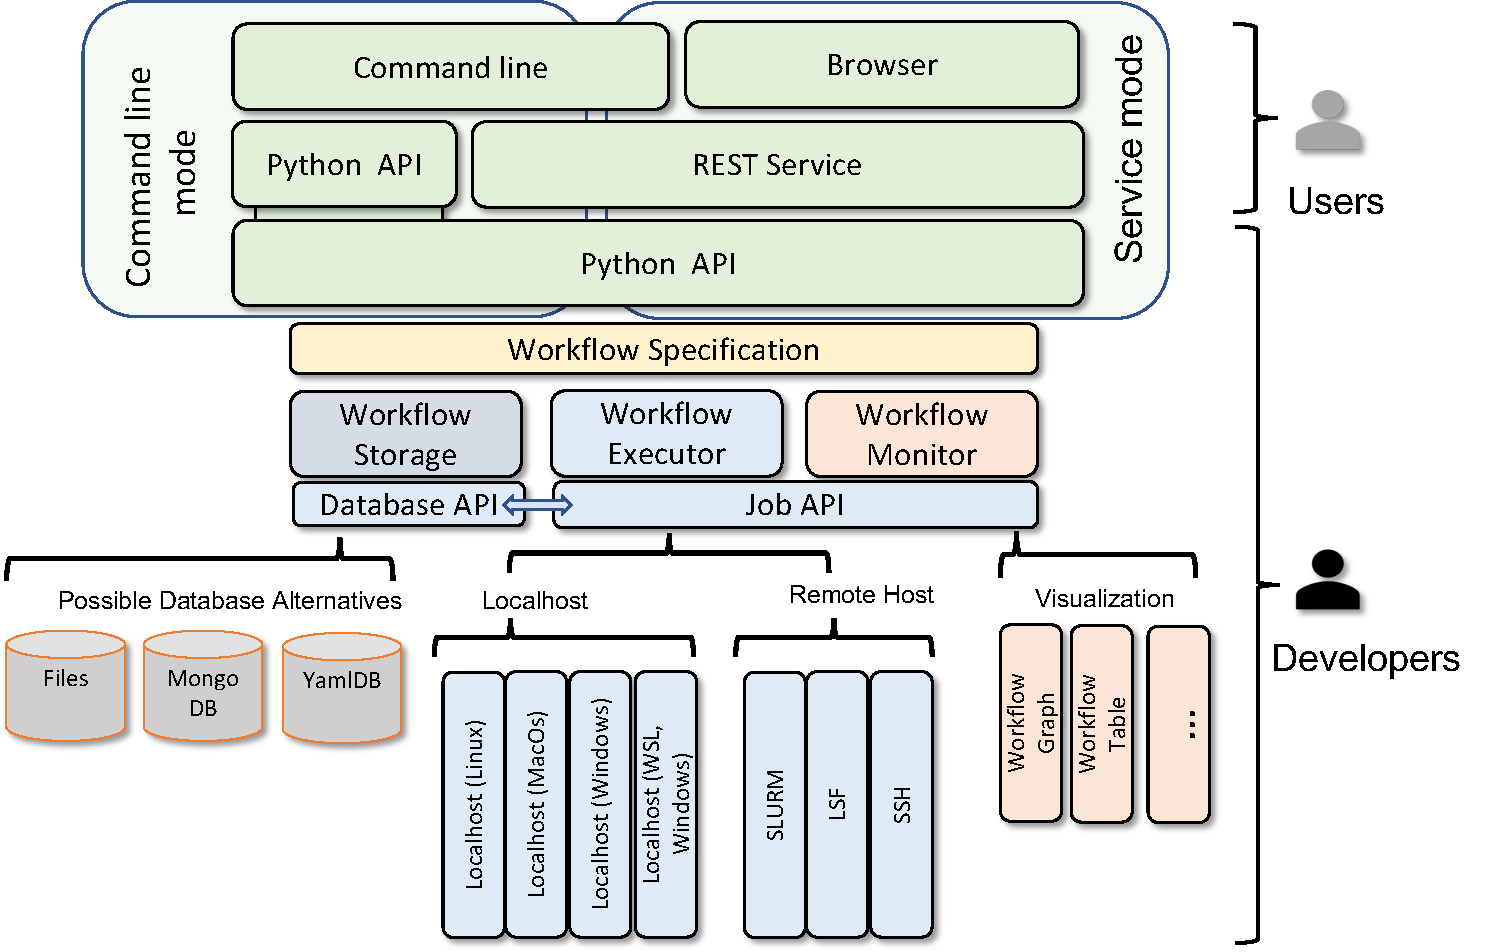
\includegraphics[width=1.0\columnwidth]{./images/cloudmesh-cc-arch.pdf}
}
\caption{Architecture of the Cloudmesh-cc Framework}\label{fig:arch}
\end{figure}



The framework is based on a layered architecture so it can be improved
and expanded on at each layer. We distinguish two kinds of users,
developers and end users, that define their workflows to run on
compute resources. For the end user, we provide a command line and a
very simple browser interface. Simplicity is important as it does not
require spending exorbitant amounts of time to learn how to use the
workflow framework. To support developers, we have designed a minimal
Python API that is also used to implement a REST Service.  Currently,
the REST Service is supposed to run on the client, but a service
deployment could also be conducted while assuring that proper
authentication and authorization are used. This is easily possible as
we use a well-known REST service framework (FastAPI) that can
integrate with common security frameworks to secure services. The API,
workflow specification, command line interface, and browser are well
documented with the help of Sphinx and OpenAPI.

The workflow specification plays an important role in not only
defining a workflow but also keeping the status of a currently
executed workflow. Here we have completely separated the status of the
workflow and synchronize the state of the workflow with pull requests
to the service that executes the computation. This allows the system
to be shut down at any time while the running jobs are completely
independent of the client application accessing the state. Thus, the
client appears to be stateless and fetches the state of the submitted
jobs on demand. It will return the latest state found on the job
execution services.

The workflows are defined with YAML. The workflow is stored in a
database that can be implemented using a variety of backends such as
YamlDB (which is file-based), MongoDB, or pickle. In our current
implementation, we simply use a file-based implementation as it is not
required to set up and manage more complex databases. This is an
important capability as we found that scientists and beginning
students do not want to engage in the hassle of setting up and
managing a datastore such as MongoDB.

As we use a YAML file to represent the status of the workflow, it is
easy to create monitoring components (for example, as part of a Web
browser). Various sophisticated graph display frameworks could be
used. For now, we have simply exposed the graph in table format using
datatables.net and the graph as SVG while leveraging Graphviz.

One of the most important parts of the framework is how we manage jobs
and monitor their status. For this, we have introduced an abstract job
class that is integrated into our workflow class. The job class can
define jobs, start them, and cancel them, to name only the most
important management methods. However, each job defines a status file
in which the actual progress of the job is recorded. This status file
is managed on the compute resource where the job is run and is queried
on demand to return the status to the client. This way, the status of
all jobs can be monitored. As our goal is not to run jobs that execute
in milliseconds, but rather in the second range, such status reporting
and propagation is well-suited for us. We have defined a special
status progress update specification that is universally
applicable. These jobs can be bash scripts, Python scripts, Jupyter
notebooks, or Slurm scripts.

Workflows are compilations of jobs to be run on nodes. These workflows
report information on the status of jobs as they are run, whether
locally or remotely. These types of jobs can be mixed with others into
a single workflow. This allows us, as already mentioned, to view the
progress of a workflow as it is being run in quasi-realtime.  The
workflow can be monitored as a graph or a DataTable. These interfaces
report the statuses of the jobs. Additionally, the order in which the
jobs are run can be specified, enabling prerequisite jobs and the
segmentation of a workflow.

To address the requirement of simplicity, the overall code is less
than 3600 lines of code, with additional 2600 lines for extensive test
cases.

The framework is managed as an open-source repository in GitHub and
uses Python as the implementation language. The code is compatible
with Windows, macOS, and Linux.

% \section{Specifying Workflows}\label{specifying-workflows}

Users of cloudmesh cc must follow a certain configuration style to best
specify how a workflow should be run. Customization options include
specifying the job types, the order of how the jobs should be run, and
the portrayal of the graph.

\subsection{Workflow YAML format}\label{workflow-yaml-format}

A workflow yaml file with three Shell script jobs \texttt{a},
\texttt{b}, and \texttt{c} is as follows:

\begin{verbatim}
```text
workflow:
  nodes:
    a:
       name: a
       user: gregor
       host: localhost
       kind: local
       status: ready
       label: '{name}\nprogress={progress}'
       script: test-a.sh
    b:
       name: b
       user: gregor
       host: localhost
       kind: local
       status: ready
       label: '{name}\nprogress={progress}'
       script: test-b.sh
    c:
      name: c
      user: gregor
      host: localhost
      kind: local
      status: ready
      label: '{name}\nprogress={progress}'
      script: test-c.sh
  dependencies:
    - a,b,c
```
\end{verbatim}

\subsection{Example Workflows}\label{example-workflows}

Sample yaml files can be found at the following link:

\url{https://github.com/cloudmesh/cloudmesh-cc/blob/main/tests/workflow-example/workflow-example.yaml}

\subsection{Defining nodes in the
workflow}\label{defining-nodes-in-the-workflow}

Nodes can be customized in various ways within the workflow
configuration YAML file, including their job types (python, sh, jupyter,
or slurm), their virtual Python environment (by specifying
\texttt{venv}), their appearance on the graph, and other
characteristics.

\subsubsection{Defining labels for the
workflow}\label{defining-labels-for-the-workflow}

These variables must be in curly braces when defining the labels inside
the yaml workflow files.

For example, a label could be defined as follows:

\begin{verbatim}
```text
workflow:
  nodes:
    start:
      label: 'start\nCreated={created.%Y/%m/%d, %H--%M--%S}\nWorkflow Started={t0.%Y/%m/%d, %H--%M--%S}\nNow={now.%Y/%m/%d, %H--%M--%S}\nElapsed={dt0.%M--%S}'
```
\end{verbatim}

This creates a node on the graph that looks similar to the following
example:

\begin{figure}
\centering
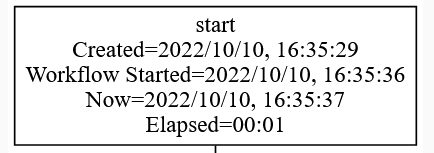
\includegraphics{images/labelmaker-example.png}
\caption{An example node with labels}
\end{figure}

Initially, the created and elapsed labels are \texttt{N/A} if the
workflow has not yet started, but they are replaced during runtime. This
can be observed by running a workflow in graph view in the web
interface.

Colons must be replaced with \texttt{-\/-} and the years, months, days,
hours, minutes, and seconds can be arranged as desired, as long as the
corresponding letters remain consistent (\texttt{\%Y} \texttt{\%m}
\texttt{\%d} \texttt{\%H} \texttt{\%M} \texttt{\%S} respectively). Also,
the format of the time must come immediately following the period.

\begin{itemize}
\tightlist
\item
  \texttt{name} name of job
\item
  \texttt{progress} progress of job from 0-100
\item
  time labels:

  \begin{itemize}
  \tightlist
  \item
    \texttt{now.} current time
  \item
    \texttt{now.\%Y/\%m/\%d,\ \%H-\/-\%M-\/-\%S} now in particular
    format (this can be used for other times as well)
  \item
    \texttt{created.} time when workflow was created
  \item
    \texttt{t0.} workflow start time
  \item
    \texttt{t1.} workflow end time
  \item
    \texttt{dt0.} elapsed time since workflow began
  \item
    \texttt{dt1.} total time of workflow once complete
  \item
    \texttt{tstart.} job start time
  \item
    \texttt{tend.} job end time
  \item
    \texttt{modified.} job modified time
  \end{itemize}
\item
  \texttt{os.} operating system environment variable (like os.HOME)
\item
  \texttt{cm.} cloudmesh variable that is read from \texttt{cms\ set}
\end{itemize}

\subsection{Defining format for timestamp
labels}\label{defining-format-for-timestamp-labels}

Various formats can be used for the timestamps, such as the American
datetime format \texttt{\%m/\%d/\%Y,\ \%H-\/-\%M-\/-\%S} or the
international datetime format \texttt{\%Y/\%m/\%d,\ \%H-\/-\%M-\/-\%S}.
As long as the letters stay consistent (\texttt{\%Y} \texttt{\%m}
\texttt{\%d} \texttt{\%H} \texttt{\%M} \texttt{\%S} for year, month,
day, hour, minute, and second, respectively), any format can be created.

If no format is specified following the period after the variable, the
datetime defaults to American format.

\subsection{Defining graphviz shapes and
styles}\label{defining-graphviz-shapes-and-styles}

Any shape and style for the nodes in the graph can be chosen, as long as
they are taken from the graphviz documentation:

\url{https://graphviz.org/doc/info/shapes.html}

\url{https://graphviz.org/docs/attr-types/style/}

The following is an example of a node in YAML format that uses a box
shape and an empty style. The empty style defaults to \texttt{filled},
which allows the node to change color when the job status is changed.

\begin{verbatim}
```text
workflow:
  nodes:
    start:
      label: 'start\nCreated={created.%Y/%m/%d, %H--%M--%S}\nWorkflow Started={t0.}\nElapsed={dt0.}'
      kind: local
      user: grey
      host: local
      status: ready
      exec: 'echo hello'
      name: start
      shape: box
      style: ''
```
\end{verbatim}

\subsection{Defining dependencies in the
workflow}\label{defining-dependencies-in-the-workflow}

Dependencies are specified in the order which jobs should be run, from
left to right. They are listed under the workflow in the yaml file.

\begin{verbatim}
```bash
workflow:
  nodes:
    a:
       name: a
    b:
       name: b
    c:
       name: c
  dependencies:
    - a,b,c
```
\end{verbatim}

\subsection{Reporting Progress}\label{reporting-progress}

When running scripts/jobs inside a workflow, the scripts must leverage
some format of cloudmesh.progress to run successfully. Otherwise, the
Workflow class cannot tell if the scripts are done, breaking the
progress functionality.

The examples that are provided with cloudmesh-cc are already augmented
with cloudmesh.progress. Thus, if a user is running self-made jobs and
workflows, they must adhere to the guidelines as follows.

\subsection{Shell and Slurm Scripts}\label{shell-and-slurm-scripts}

For shell and Slurm scripts \texttt{.sh}, the script must contain:

\begin{verbatim}
```bash
echo "# cloudmesh status=running progress=1 pid=$$"
```
\end{verbatim}

at the beginning of the script, and

\begin{verbatim}
```bash
echo "# cloudmesh status=done progress=100 pid=$$"
```
\end{verbatim}

at the end of the script.

\subsection{Python Scripts and Jupyter
Notebooks}\label{python-scripts-and-jupyter-notebooks}

For Python scripts \texttt{.py} and Jupyter notebooks \texttt{.ipynb},
the script must contain an import module from cloudmesh.common and calls
to the progress function.

py\_script.py

\begin{verbatim}
```bash
from cloudmesh.common.StopWatch import progress
from cloudmesh.common.Shell import Shell
filename = Shell.map_filename('./py_script.log').path
progress(progress=1, filename=filename)

# your script does what you want it to do here...

progress(progress=100, filename=filename)
```
\end{verbatim}

The statements do not need to be at the absolute beginning or end of the
script, but the progress must:

\begin{itemize}
\tightlist
\item
  be written to a filename with the same name as the script, ending in
  \texttt{.log}
\item
  begin at progress=1
\item
  and end at progress=100
\end{itemize}



\FILE{specifying-workflows.tex}

\section{Specifying Workflows}\label{specifying-workflows}

The workflow definition for cloudmesh is rather simple and intuitive.
An example is provided in Figure~\ref{fig:workflow-example}. Here, a
DAG with three nodes are specified ($start \rightarrow fetch-data
\rightarrow compute \rightarrow analyze \rightarrow end$). The
workflow executes three scripts
(test-[fetch-data,compute,analyze].sh). It contains a specific start
and end node.

\subsection{Dependencies}

Each dependency is specified in the {\em dependency} section while
providing sequences of names in a list such as
{\scriptsize\texttt -start,fetch-data}
or, in our case where 3 more nodes are defined,
additional nodes are appended with commas, as in
{\scriptsize\texttt ,compute,analyze,end}.

In case one wants to execute nodes in parallel, we can simply define
them through a list such as 


{\scriptsize
\begin{verbatim}
  dependencies:
    - start,a,end
    - start,b,end
    - start,c,end
\end{verbatim}
}

if the names of the nodes were $a$, $b$, and $c$. 

\subsection{Nodes}

Nodes can be customized in various ways within the workflow
configuration YAML file, including their job types (python, sh,
jupyter, or slurm), their virtual Python environment (by specifying
{\scriptsize\texttt venv}), their appearance on the graph, and other
characteristics. This is controlled through a number of attributes
used by the nodes in the DAG. The attributes are summarized in
Table~\ref{tab:node-attributes}.

\begin{figure}
{\scriptsize
\begin{verbatim}
workflow:
  nodes:
    start:
       name: start
    fetch-data:
       name: fetch-data
       user: gregor
       host: localhost
       kind: local
       status: ready
       label: '{name}\nprogress={progress}'
       script: test-fetch-data.sh
    compute:
       name: compute
       user: gregor
       host: localhost
       kind: local
       status: ready
       label: '{name}\nprogress={progress}'
       script: test-compute.sh
    analyze:
      name: analyze
      user: gregor
      host: localhost
      kind: local
      status: ready
      label: '{name}\nprogress={progress}'
      script: test-analyze.sh
    end:
       name: end
  dependencies:
    - start,fetch-data,compute,analyze,end
\end{verbatim}}
\caption{Workflow YAML Configuration file.}\label{fig:workflow-example}
\label{fig:yaml-file}
\end{figure}

\begin{table}[htb]
\caption{Node attributes.}\label{tab:node-attributes}
\resizebox{1.0\columnwidth}{!}{
\begin{tabular}{|l|p{6cm}|}
\hline
{\bf Attribute} & {\bf Description} \\
\hline
\hline
name &  A unique name of the job, must be the same as defined in the : line \\
\hline
user &  The username for the host \\
\hline
host &  The hostname \\
\hline
kind &  The kind of the job, which can be local, ssh, wsl, or slurm  \\
\hline
status &  The status of the job in integer value between 0 and 100 \\
\hline
label &  A custom-designed label \\
\hline
script &  The script name to be executed \\
\hline
\end{tabular}
}
\end{table}

\subsection{Node labels}

One particular useful attribute is that of a label. If no label is
used, the name of the node is used as the label. However, if a label
is specified, one can also use attribute names and timers to create
labels with implicit state information. This is done by introducing
variables through curly braces when defining the labels inside the
label defined in nodes within the YAML workflow file.

For example, a label could be defined as showcased in
Figure~\ref{fig:label-job}. The appropriate values will be dynamically
replaced during the execution of the workflow.  This creates a node on
the graph that looks similar to the node showcased in
Figure~\ref{fig:label-node}.

Initially, the created and elapsed labels are {\scriptsize\texttt N/A}
if the workflow has not yet started, but they are replaced during
runtime. This can be observed by running a workflow in graph view in
the web interface.

In this format, we must use two dashes {\scriptsize\texttt --} to
separate the various components. However, when rendered, the dashes
will be replaced with a colon. Thus you can easily use years, months,
days, hours, minutes, and seconds can be arranged as desired, as long
as the corresponding letters remain consistent:
({\scriptsize\texttt \%Y} 
{\scriptsize\texttt \%m}
{\scriptsize\texttt \%d} 
{\scriptsize\texttt \%H} 
{\scriptsize\texttt \%M} 
{\scriptsize\texttt \%S}).
The time format must be specified immediately following the period
after a format-supported time variable.  If no format is specified
following the period after the variable, the datetime defaults to the
American format.  See Table~\ref{fig:labels-list} for a summary of
options for defining time based attributed to being replaced in the
label.


Nodes can be customized in various ways within the workflow
configuration YAML file, including their job types (python, sh,
jupyter, or slurm), their virtual Python environment (by specifying
{\scriptsize\texttt venv}), their appearance on the graph, and other
characteristics.


\begin{figure}
\smallskip
    {\scriptsize
    \begin{verbatim}
    workflow:
      nodes:
        start:
          label: 'start\n
                  Created={created.%Y/%m/%d, %H--%M--%S}\n
                  Workflow Started={t0.%Y/%m/%d, %H--%M--%S}\n
                  Now={now.%Y/%m/%d, %H--%M--%S}\n
                  Elapsed={dt0.%M--%S}'
    \end{verbatim}}
    \caption{Example of job label in YAML configuration file.}
    \label{fig:label-job}

\centering
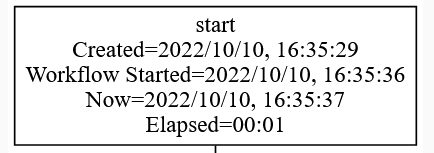
\includegraphics[width=0.7\columnwidth]{./images/labelmaker-example.png}
\caption{An example node with labels.}\label{fig:label-node}
\end{figure}

\begin{table}[htb]
\caption{List of possible labels for nodes on the graph.}
\label{fig:labels-list}

{\footnotesize
  \begin{tabular}{|p{3.5cm}|p{4cm}|}
    \hline
    {\bf Name} & {\bf Description} \\
    \hline
    \hline
    progress &  progress of job from 0-100 \\
    \hline
    now & current time \\
    \hline
    now.\verb|%Y%m%d,%H--%M--%S| &
   now in particular format (this can be used for other times as well) \\
    \hline
    created & time when workflow was created \\
    \hline
    t0.\verb|%Y%m%d,%H--%M--%S| &  workflow start time \\
    \hline
    t1.\verb|%Y%m%d,%H--%M--%S| & workflow end time \\
    \hline
    dt0.\verb|%Y%m%d,%H--%M--%S| & elapsed time since workflow began \\
    \hline
    dt1.\verb|%Y%m%d,%H--%M--%S| & total time of workflow once complete \\
    \hline
    tstart.\verb|%Y%m%d,%H--%M--%S| & job start time \\
    \hline
    tend.\verb|%Y%m%d,%H--%M--%S| & job end time \\
    \hline
    modified.\verb|%Y%m%d,%H--%M--%S| & job modified time \\
    \hline
    os. & operating system environment variable (like os.HOME) \\
    \hline
    cm. & cloudmesh variable that is read from \verb|cms set| \\
    \hline
\end{tabular}
}
\end{table}



\subsection{Shapes and Styles}

As we use graphviz for rendering, we have also added the ability to
change the shape and style of each node in the graph. The
available \href{https://graphviz.org/doc/info/shapes.html}{shapes}
and \href{https://graphviz.org/docs/attr-types/style/}{styles} are
listed in the Graphviz documentation \cite{www-graphviz}.

Figure~\ref{fig:shape-style-yaml} is an example of a node in YAML
format that uses a box shape and an empty style. The empty style
defaults to \verb|filled|, which allows the node to change
color when the job status is changed.

\begin{figure}
    {\scriptsize
    \begin{verbatim}
    workflow:
      nodes:
        start:
          label: 'start\n
                  Created={created.%Y/%m/%d, %H--%M--%S}\n
                  Workflow Started={t0.}\n
                  Elapsed={dt0.}'
          kind: local
          user: grey
          host: local
          status: ready
          exec: 'echo hello'
          name: start
          shape: box
          style: ''
    \end{verbatim}}
    \caption{Example of YAML config file that uses shape and style.}
    \label{fig:shape-style-yaml}
\end{figure}



\subsection{Reporting Progress}\label{reporting-progress}

When running scripts/jobs inside a workflow, the scripts must leverage
some format of {\em cloudmesh.progress} to notify the user and the
backend client monitoring system. If progress is not reported, the
Workflow class cannot tell if the scripts are done.

The examples that are provided with cloudmesh-cc are already augmented
with {\em cloudmesh.progress}. Thus, if a user is running jobs through
cloudmesh cc workflows, they must integrate progress strings into the
log files that are monitored. This is available for shell, batch,
Python, and Jupyter scripts.

For shell and Slurm scripts, the script must contain a progress update
lines as follows:

{\scriptsize
\begin{verbatim}
  echo "# cloudmesh status=running progress=1 pid=$$"
\end{verbatim}
}

\parindent0pt at the beginning of the script, and

{\scriptsize
\begin{verabtim}
  echo "# cloudmesh status=done progress=100 pid=\$\$"
\end{veratim}
}

at the end of the script.

For Python scripts and Jupyter notebooks, it is easiest to use our
built-in progress method and import it from the cloudmesh.common
module as the example in Figure~\ref{fig:py-progress}. 

\begin{figure}[htb]

{\scriptsize
\begin{verbatim}
  from cloudmesh.common.StopWatch import progress
  from cloudmesh.common.Shell import Shell
  filename = Shell.map_filename('./py_script.log').path
  progress(progress=1, filename=filename)
  # execute your analysis here ...
  progress(progress=100, filename=filename)
\end{verbatim}}
\caption{Progress report with the cloudmesh Python API.}
\label{fig:py-progress}

\end{figure}


When recording progress, the progress should be ascending between 1
and 100. The last value must report 100 or the node will not be
completed and the workflow gets stuck. The output of the progress will
be written into a {\scriptsize \verb|{workflowname}.log|} file that
will be probed continuously by the client to report the progress to
the user.

\subsection{Generating Progress Image as Graph}

The framework has a built-in capability to export the progress of the
workflow in a DAG.

In Figure~\ref{fig:workflow-process}, we depict a simple example
workflow to be executed, where each task is executed sequentially. The
status of the execution can be displayed as a table or as a graph. In
Figure~\ref{fig:workflow-process}, we showcase how the graph changes
its appearance over time while using no label in the start and end
node and a defined label in the nodes for fetch-data, compute, and
analyze:

{\scriptsize
\begin{verbatim}
  label: "{name}\nprogress={progress}"
\end{verbatim}
}

\begin{figure}[htb]
\resizebox{1.0\columnwidth}{!}{
\begin{minipage}[b]{0.18\textwidth}
Definition and start \\
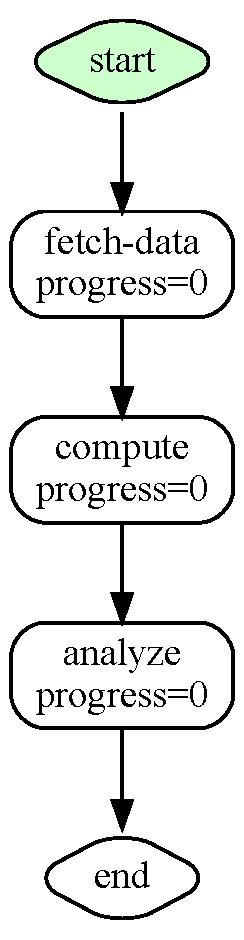
\includegraphics[height=9cm]{./images/workflow-example-1.pdf}
\end{minipage} \ \
\begin{minipage}[b]{0.18\textwidth}
Running 1st task \\
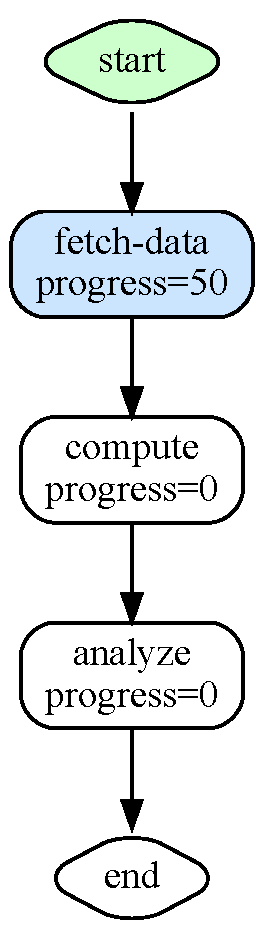
\includegraphics[height=9cm]{./images/workflow-example-1.5.pdf} 
\end{minipage} \ \
\begin{minipage}[b]{0.18\textwidth}
Complete 1st task \\
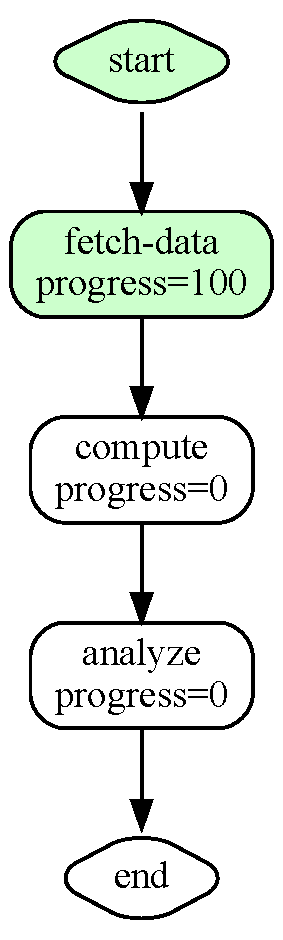
\includegraphics[height=9cm]{./images/workflow-example-2.pdf}
\end{minipage} \ \
\begin{minipage}[b]{0.18\textwidth}
Complete 2nd task \\
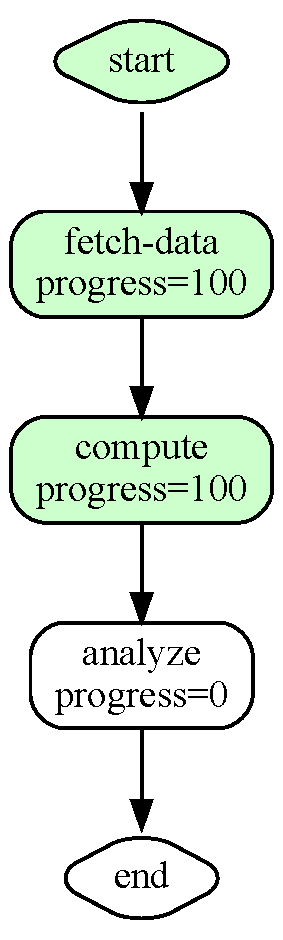
\includegraphics[height=9cm]{./images/workflow-example-3.pdf}
\end{minipage} \ \
\begin{minipage}[b]{0.18\textwidth}
Complete workflow \\
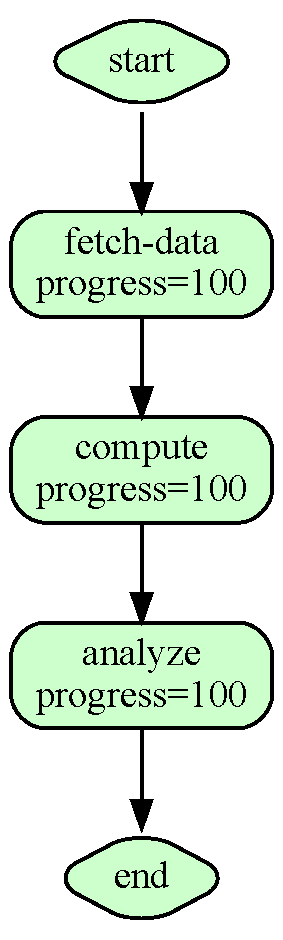
\includegraphics[height=9cm]{./images/workflow-example-5.pdf}
\end{minipage} 
}
\caption{The gradual process of a simple workflow.}\label{fig:workflow-process}
\end{figure}





% \FILE{quickstart.tex}

\section{Cloudmesh-cc Interfaces}

In this section we explain the various ways of interfacing with cloudmesh-cc.

It is important to note that we have a {\em commandline mode} that interfaces directly with the backends while not requiering a service. This includes an easy to use python API.

In addition we have used this API to implement a {\em service mode}, so we an stand up a REST service as well as a GUI that can ba accessed through a Web browser.
Please note that the service mode can also be access through te command line in a terminal. To distinguish how we operate cloudmesh-cc we use the term {\em mode} to deliniate it from a command that is entered ina terminal to query the status of the workflow.

We will now discuss tes interfaces in more detail and also showcase
hwo we can access them.


\subsection{Python API}

Cloudmesh-cc is implemented in Python. Extensive documentation is
available in GitHub and through GitHub action it is automatically
updated \cite{github-cloudmesh-cc}.  We distingush two main classes
that are easy to use. The first is a {\em Job class} that can adapted
to include new computational resource types for executing jobs. The
second is a {\em Workflow class} to ccordinate the execution of
multiple jobs. Selected methods of the Job class include are listed in
Figure~\ref{fig:code-job}. Important to note is that the code for the
scripts are all managed locally and a synchronization step is invoked
prior to one running the job to assure that the latest script and
code to be executed on the compute resource is available.

The most important part of using the Workflow Python API is showcased
in Figure~\ref{fig:code-job}, where we explain how easy it is to set up a workflow
with the Python API.

\begin{figure}[!h]
\begin{minted}[breaklines]{bash}
class Job:
   ...
   def clear():
      """Clear job progress."""
   def create(filename=None, script=None, exec=None):
      """Create a template for the script with progress."""
   def get_log(refresh=True):
      """Get the log of the job."""
   def get_pid(refresh=False):
      """Get the pid that the job is running within determined by the compute resource it is running on."""
   def get_progress(refresh=False):
       """Get the progress of the job from the compute resource."""
   def get_status(refresh=False):
       """Get the status of the job."""
   def kill():
       """Kill the job."""
   def run():
       """Run the job."""
   def sync():
       """Synchronise the current directory with the remote. Copies the shell script to the experiment directory and ensures that the file is copied with the sync command."""
   def watch(period=10):
       """Watch the job and check for changes in the given period."""
\end{minted}
\caption{Pseudo code for the Job class with selected methhods}
\label{fig:code-job}

\bigskip

\begin{minted}[breaklines]{bash}
class Workflow:
    ...
    def add_dependencies(dependency)
        """Add a job dependency to the workflow (and the graph)."""
    add_dependency(source, destination)
        """Add a job dependency to the workflow (and the graph)."""
    def add_job( ... ):
        """Add a job to the workflow with appropriate parameters."""
    def display(filename=None, name='workflow', first=True)
        """Show the graph of the workflow."""
    def job(name):
        """Return the details of a job within the workflow."""
    def load(filename, clear=True)
        """Load the workflow."""
    def remove_job(name, state=False)
        """Remove a particular job from the workflow."""
    def remove_workflow()
        """Delete workflow from the local file system."""
    def run_parallel( ... )
        """Run a workflow in a parallel fashion."""
    def run_topo(order=None, dryrun=False, show=True, filename=None)
        """Run the workflow in a topological order."""
    def save(filename=None):
        """Save the workflow."""
    def save_with_state(filename, stdout=False):
        """Save the workflow with state."""
    def sequential_order():
        """Return a list of the topological order of the workflow."""
    property table
        """Return a table of the workflow."""
    def update_progress(name):
        """Manually update the progress of a job according to its log file."""
    def update_status(name, status):
        """Manually update a job’s status."""
\end{minted}
\caption{Pseudo code for the Job class with selected methhods}
\label{fig:code-workflow}
\end{figure}


\begin{figure}[htb]
\begin{minted}[breaklines]{bash}
    w = Workflow(name="workflow-analyze")
    # load a preexisting workflow
    # w.load(filename="source.yaml")
    
    # add jobs and dependencies explicitly
    w.add_job(name="fetch-data",
              exec="hostname",
              host='supercomputer-a' # defined in .ssh
              label="{name}\nprogress={progress}",
              kind="local",
              status="ready",
              progress=0)
    w.add_job(name="compute", command="... TBD ...")
    w.add_job(name="analyze", command="... TBD ...")
    w.add_dependencies(
              dependency="start,fetch-data,compute,analyze")
    w.run_topo()
\end{minted}
\caption{Pseudo code for the Job class with selected methods}
\label{fig:code-workflow-example}

\bigskip

\begin{minted}[breaklines]{bash}
      cms cc workflow add [--name=NAME] [--job=JOB] ARGS...
      cms cc workflow add [--name=NAME] --filename=FILENAME
      cms cc workflow delete [--name=NAME] [--job=JOB]
      cms cc workflow list [--name=NAME] [--job=JOB]
      cms cc workflow run [--name=NAME] [--job=JOB] [--filename=FILENAME]
      cms cc workflow [--name=NAME] --dependencies=DEPENDENCIES
      cms cc workflow status --name=NAME [--output=OUTPUT]
      cms cc workflow graph --name=NAME
\end{minted}
\caption{Command line interface to the workflow in terminal mode}
\label{fig:code-workflow-commandline}

\bigskip

\begin{minted}[breaklines]{bash}
      cms cc start [-c] [--reload] [--host=HOST] [--port=PORT]
      cms cc stop
      cms cc status
      cms cc workflow service add [--name=NAME] FILENAME
      cms cc workflow service list [--name=NAME] [--job=JOB]
      cms cc workflow service add [--name=NAME] [--job=JOB] ARGS...
      cms cc workflow service run --name=NAME
\end{minted}
\caption{Command line interface to the workflow in service mode}
\label{fig:code-workflow-service-commandline}.

% \bigskip

{\centering
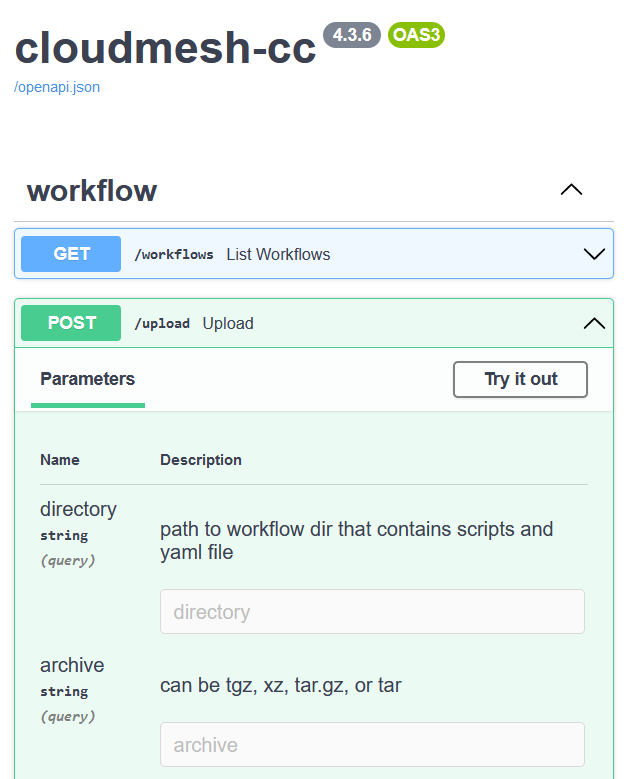
\includegraphics[width=0.52\columnwidth]{images/upload_api.png}
}
\caption{Browser API GUI for Cloudmesh Compute Cluster}

\label{fig:openapi}

\end{figure}


\subsection{Commandline Mode}

The commandline mode is an implementation that does not use a backend
service. It runs in the terminal until the workflow is completed. All
states of the jobs are managed on the compute service on which the job
is run and the status is replicated into the client on demand. This
allows easy reporting of the status through a table and a graph
display using client based rendering tools. The various commands to
interact with it on the commandline are shown in
Figure~\ref{fig:code-workflow-commandline}.


\subsection{Service Mode}

The Python API has ale been used to implement a REST service. To
easily interact with the REST service we have also added a couple of
conveneinet commannds one can issue from a terminal. They are listed
in Figure~\ref{fig:code-workflow-service-commandline}. It is clear for
these methods that starting stopping and getting the status of the
service is very easy, In contrast to the commandline mode this service
mode has an additional keyword {\em service} to interact with the rest service.

Certainly one can also directly interact with the REST service API for
this service. For ease of use we have exposed the interface through
an OpenAPI specification that is available to the user as shown in
Figure~\ref{fig:openapi}.



Thus other tools such as curl or other languages supporting url
requests can be used. A curl example to list the workflow
specifications uploaded to the service is

As we use a REST service, we can also easily upload the workflow
through a Python enabled REST call. We will use Python requests to
demonstrate this upload feature. To showcase the various ways to
access the service we focus on uploading a tar file that contains the workflow as well as the scripts or programs used in the workflow. The tar file is called {\em workflow.tar}

To also allow programming against the REST service in Python a Python
API similar to that pf the commandline mode is
available. Figure~\ref{fig:code-workflow-rest-commandline} showcases
this API.

To simplify interaction with the Rest service we create a special
RESTWorkflow class that is similar to the command module API but uses
instead the REST interface to the service rather than directly
communication with the command client API.

If the user wants to use instead just Python requests he can do so as
follows, while we just showcase the program in
Figure~\ref{fig:code-workflow-requests} for uploading.

\begin{figure}[t]
\begin{minted}[breaklines]{bash}
class RESTWorkflow
    ...
    def add_job(workflow_name, **kwargs):
        """Add a job to the workflow."""
    def delete_workflow(workflow_name, job_name=None):
        """Delete a workflow by using REST."""
    def get_workflow(workflow_name, job_name=None):
        """Retrieve a workflow by using REST."""
    def list_workflows():
        """Return a list of workflows that is found within
           the server."""
    def run_workflow( ... ):
        """Run a workflow by using REST."""
    def upload_workflow( ... ):
        """Upload a workflow by using REST."""
\end{minted}
\caption{Pseudo code for the Job class with selected methods}
\label{fig:code-workflow-rest-commandline}

\bigskip

\begin{minted}[breaklines]{python}
import requests
r = requests.post(
      'http://127.0.0.1:8000/workflow?archive=workflow-example.tar')
print(r.text)
\end{minted}
\caption{Upload to the REST service with Python requests}
\label{fig:code-workflow-requests}

\bigskip

\begin{minted}[breaklines]{bash}
$ curl -X 'POST' 'http://127.0.0.1:8000/ workflow?archive=workflow-example.tar'                           -H 'accept: application/json' -d ''
\end{minted}%$
\caption{Upload to the REST service with curl}
\label{fig:code-workflow-curl}

\end{figure}


\subsection{Webservice GUI}

A convenient Web service is included in Cloudmesh cc. It allows the user
to manage and visualize the status of workflows through a Web browser
interface. At this time the focus is that the interface can be run by a
singleuser on the local machine. This allows that remote executions of
workflow nodes run completely independent from cloudmesh cc and
interaction is possible in asynchronous mode.

As the service is using also an OpenAPI 2.0 specification the workflow
can also be uploaded implicitly through the specification
GUI. Navigate to \texttt{http://127.0.0.1:8000/docs} and use the POST
Upload method. Then click \texttt{Try\ it\ out} and enter the
location of the tar file, followed by clicking {\em Execute}.

Obviously, any REST service or REST API can be used allowing to
interface to it from different programming languages or frameworks.

The web server provides a more customizable, easy-to-use interface for
the Workflow class which can be started, viewed, and stoped with the
appropriate command line. 

\begin{minted}[breaklines]{bash}
  $ cms cc start
  $ cms cc view
  $ cms cc stop
\end{minted}%$

The view can also be achieved by opening the 
the link {\scriptsize \verb|http://127.0.0.1:8000/}.

Now the browser provides an interface to view preexisting workflows in both
a DataTable format and as a graph format. Both views will update
automatically, in a live fashion, as the workflows are run, reporting
live job status and progress.

For a quick and easy example of leveraging this GUI interface, click
on the Example tab in the left-hand sidebar. Then, a workflow-example
will appear underneath Workflows. Click on the workflow-example and
run the workflow by clicking the green Run button in the top-right. As
the workflow runs, the user is able to click on the Graph button (see
Figure~\ref{fig:graph}) and back to the Table button (see
Figure~\ref{fig:table}, as desired, to view the workflow's
progression.


\begin{figure}[htb]
{\centering
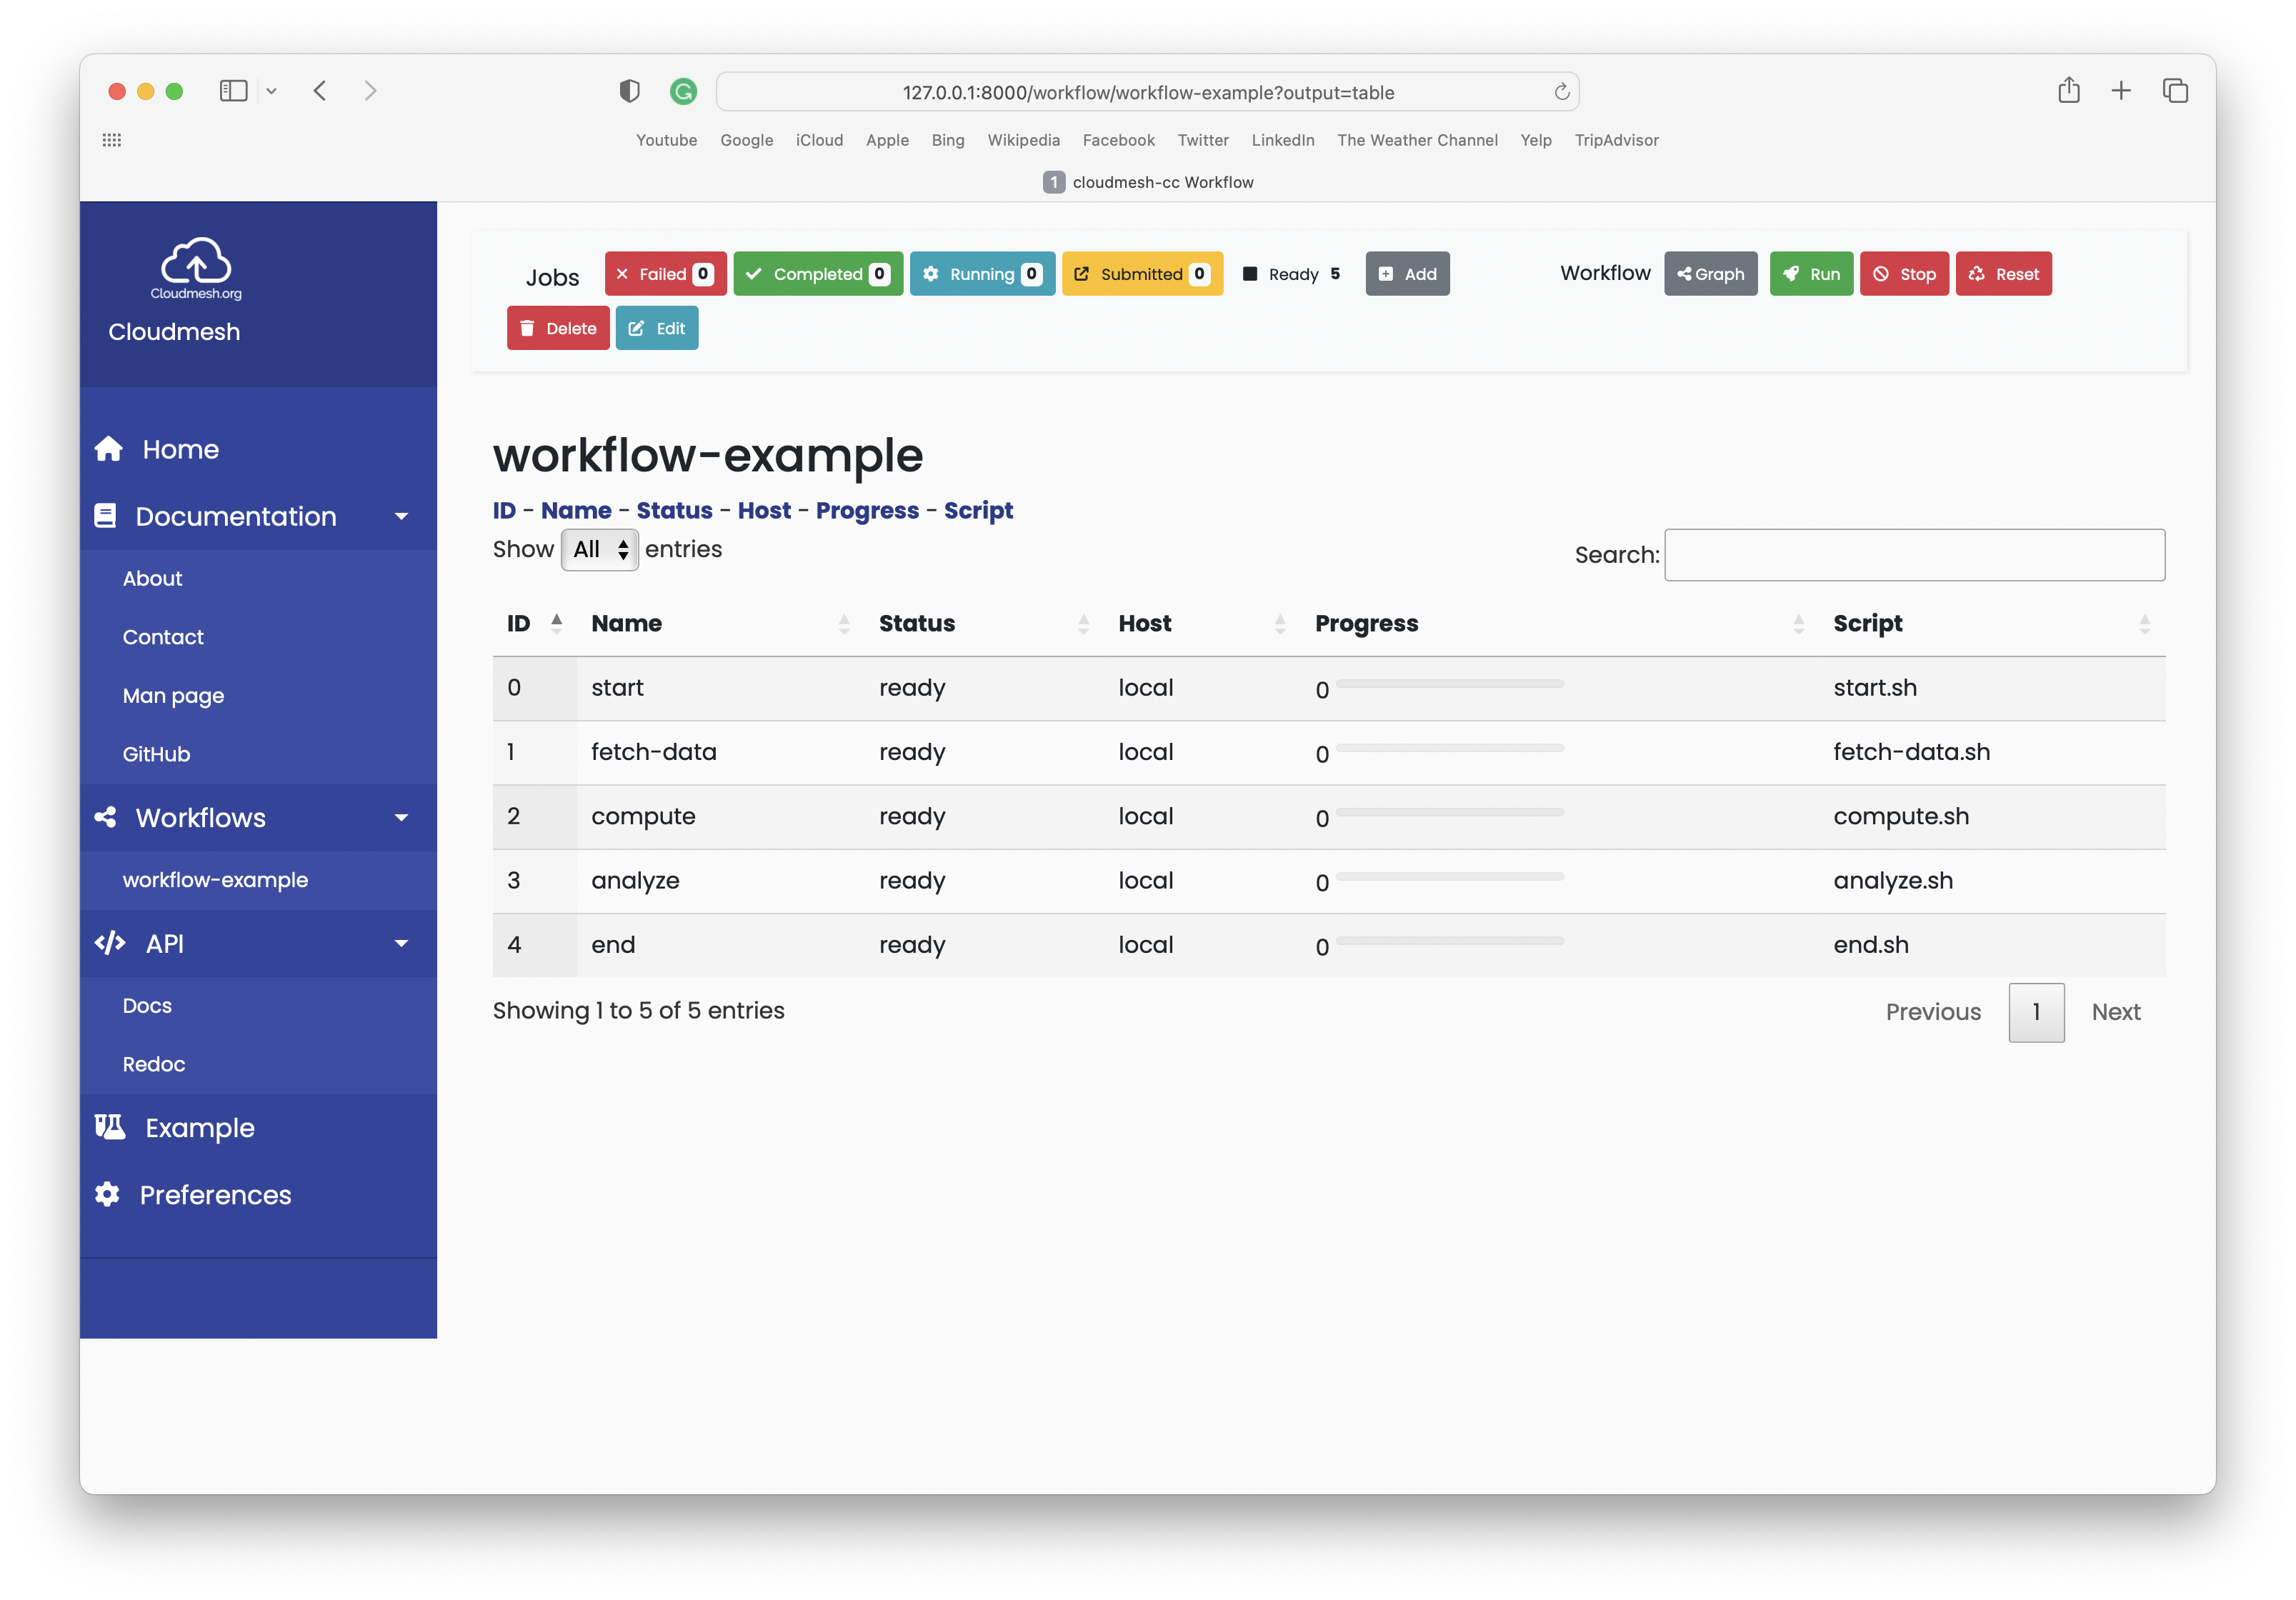
\includegraphics[width=1.05\columnwidth]{images/service-table.png}}
\caption{Cloudmesh cc workflow table view}\label{fig:table}

{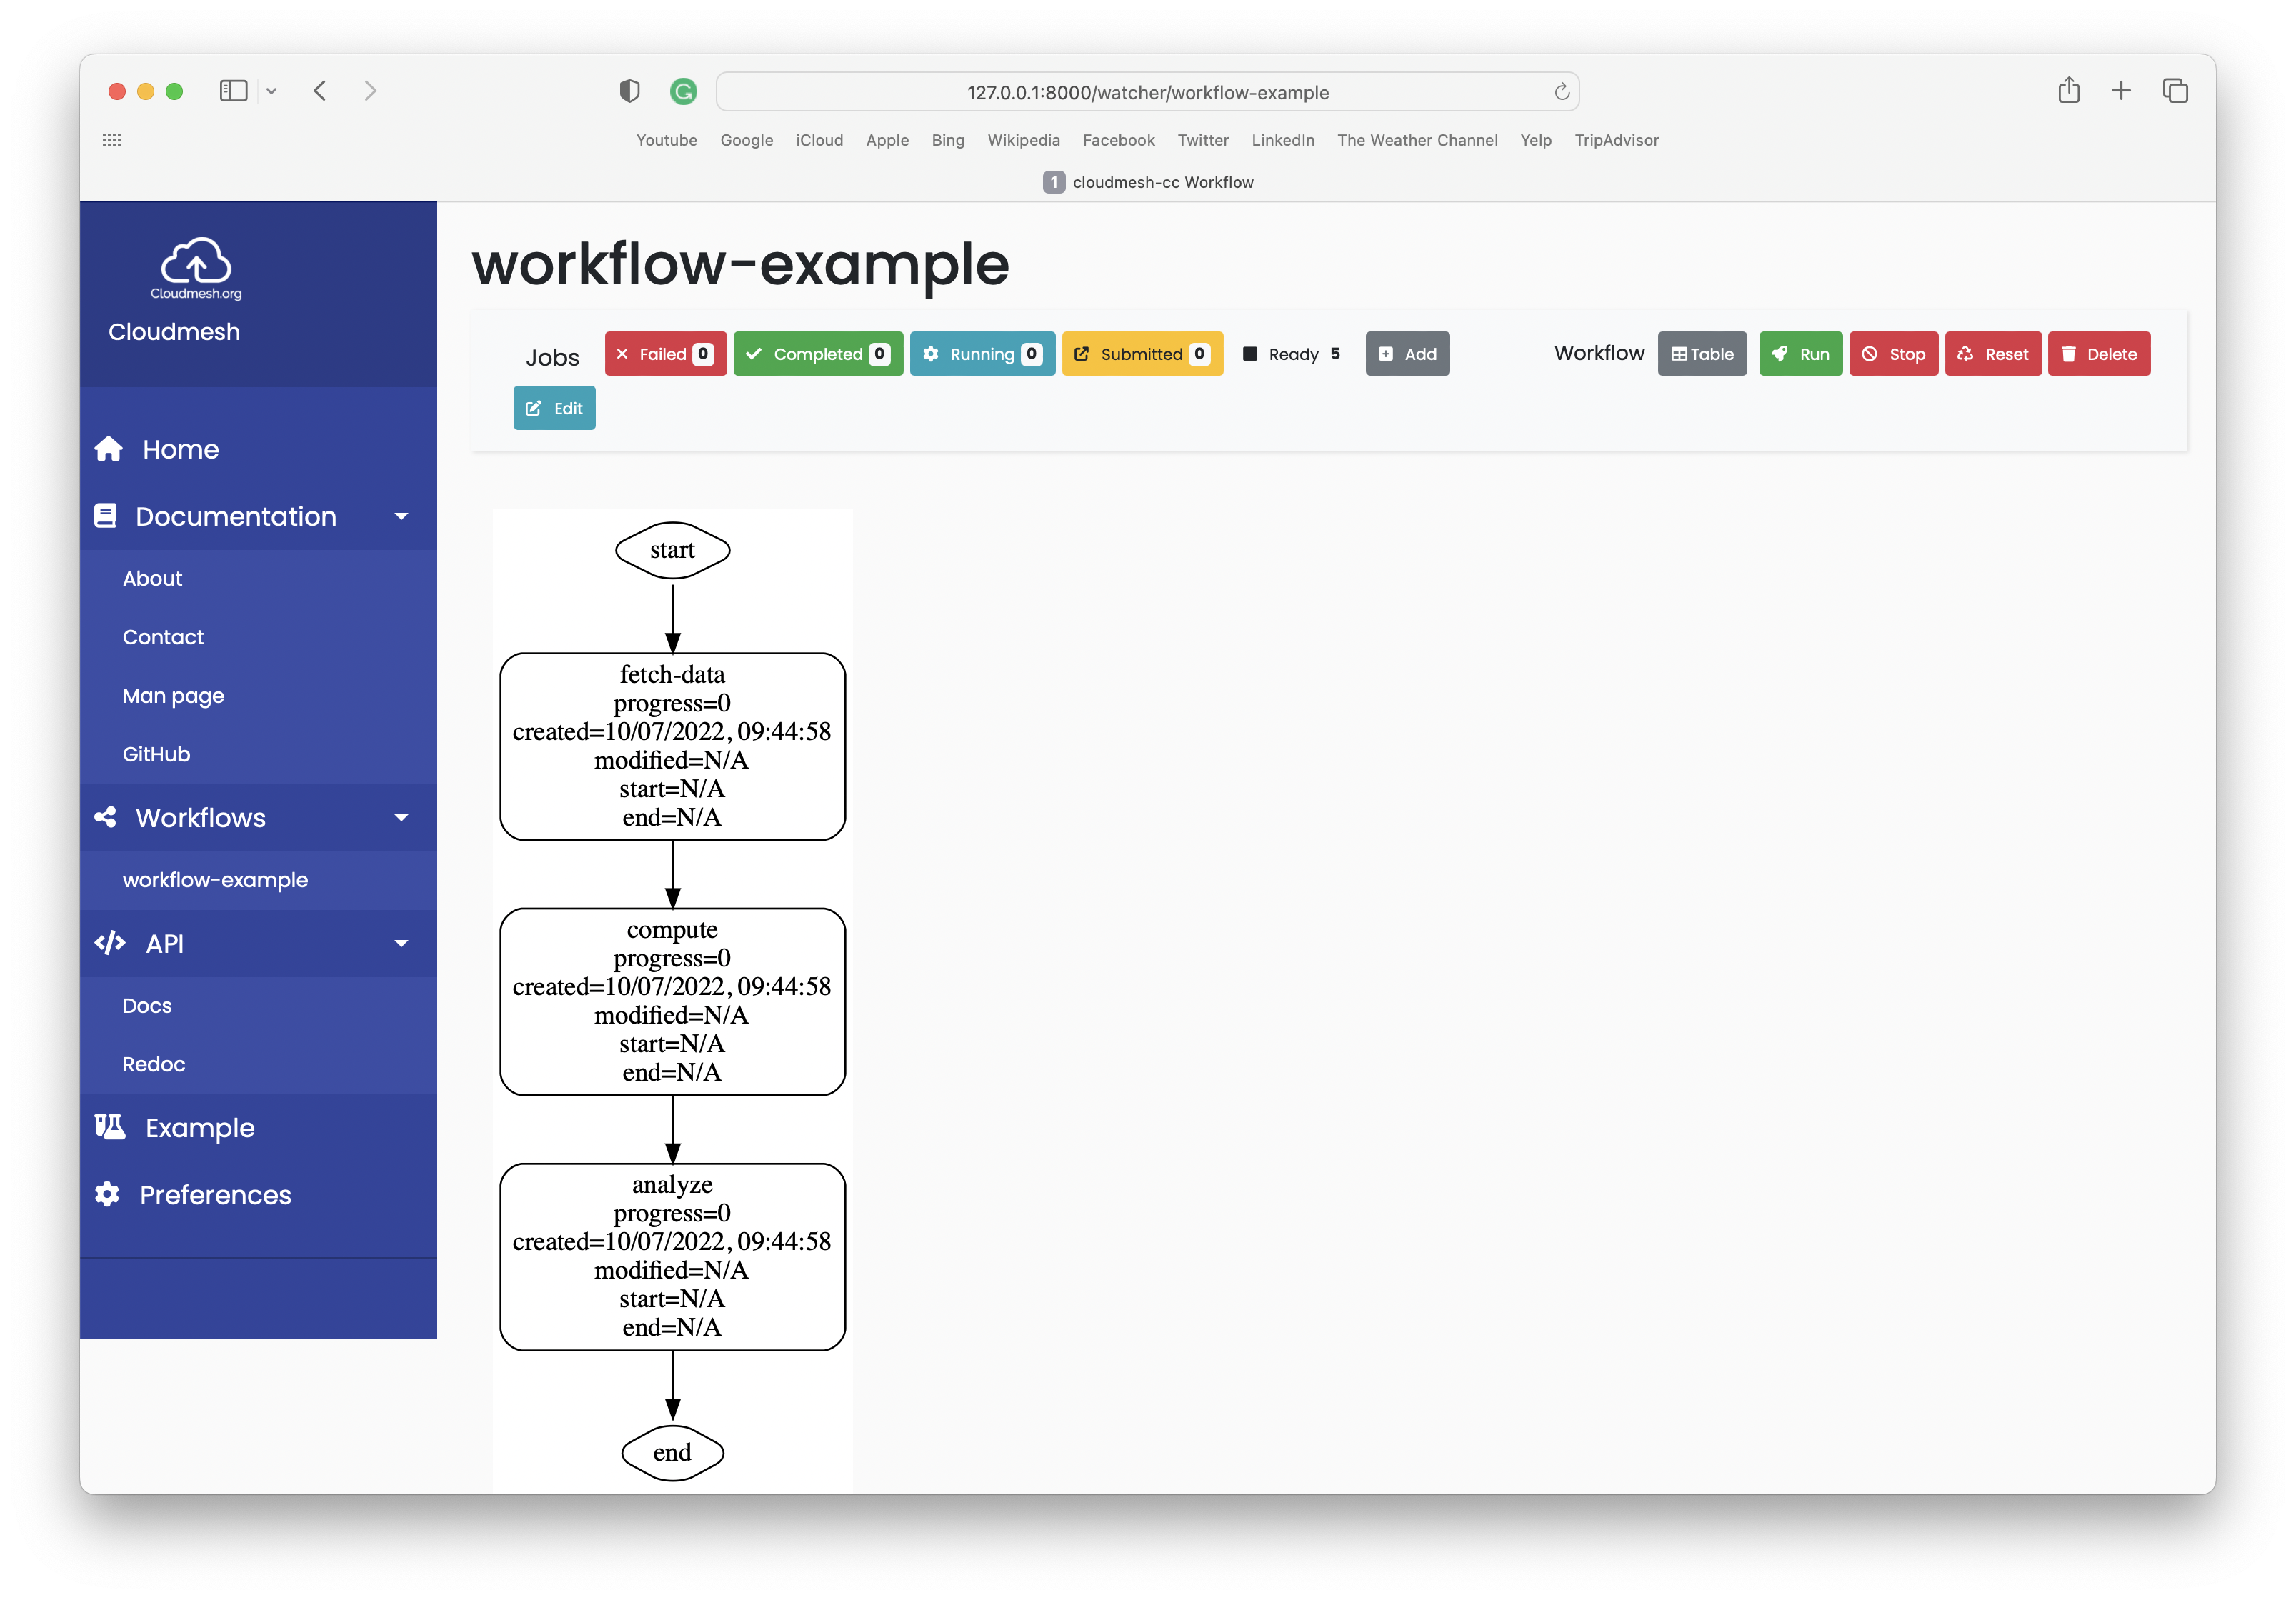
\includegraphics[width=1.05\columnwidth]{images/service-graph.png}
  \caption{Cloudmesh cc workflow graph view}}
\label{fig:graph}
\end{figure}



\subsection{Run the workflow}\label{run-the-workflow}

To run a workflow, you can use the various interfaces to do so. As an
example we will showcase here how to run is in the service mode bey
either the GUI or a curl call.

\paragraph{GUI.} To run, navigate to homepage at
\texttt{http://127.0.0.1:8000/} and click the workflow-example on the
left side. Then click Run.


\paragraph{Curl.} to run a workflow with curl please use

\begin{minted}[breaklines]{bash}
$ curl -X 'GET' 'http://127.0.0.1:8000/workflow/run/workflow-example
?show=True' -H 'accept: application/json'
\end{minted}%$

\paragraph{RESTWorkflow API}

To run the workflow with the Python cloudmesh REST API, please use the code

\begin{minted}[breaklines]{python} 
from cloudmesh.cc.workflowrest import RESTWorkflow
rest = RESTWorkflow()
result = rest.run_workflow('workflow-example')
\end{minted}

\paragraph{Python request API.} To run the workflow with the Python
request API, please use the code

\begin{minted}[breaklines]{python}
import requests
url = f'http://127.0.0.1:8000/workflow/run/workflow-example?show=True'
r = requests.get(url)
print(r)
\end{minted}








\FILE{interfaces.tex}

\section{Cloudmesh-cc Interfaces}

In this section, we explain the various ways of interfacing with
cloudmesh-cc that are part of our design (see Figure~\ref{fig:arch}).

It is important to note that we have a {\em command line mode} that
interfaces directly with the backends while not requiring a
service. This includes an easy-to-use Python API.

In addition, we have used this API to implement a {\em service mode}, so we can
stand up a REST service as well as a GUI that can be accessed through a Web browser.
Please note that the service mode can also be accessed through the command line
in a terminal. To distinguish how we operate cloudmesh-cc, we use the term
{\em mode} to delineate it from a command that is entered in a terminal to
query the status of the workflow.

We will now discuss these interfaces in more detail and also showcase
how we can access them.


\subsection{Python API}

Cloudmesh-cc is implemented in Python. Extensive documentation is
available in GitHub and, using GitHub Actions, it is automatically
updated~\cite{github-cloudmesh-cc}. We distinguish two main classes
that are easy to use. The first is a {\em Job class} that can be
adapted to include new computational resource types for executing
jobs. The second is a {\em Workflow class} to coordinate the execution
of multiple jobs. Selected methods of the Job class include are listed
in Figure~\ref{fig:code-job}. Important to note is that the code for
the scripts are all managed locally, and a synchronization step is
invoked prior to one running the job to assure that the latest script
and code to be executed on the compute resource is available.

The most important part of using the Workflow Python API is showcased
in Figure~\ref{fig:code-job}, where we explain how easy it is to set
up a workflow with the Python API.

\begin{figure}[!h]
{\scriptsize
\begin{verbatim}
class Job:
   ...
   def clear():
      """Clear job progress."""
   def create(filename=None, script=None, exec=None):
      """Create a template for the script with progress."""
   def get_log(refresh=True):
      """Get the log of the job."""
   def get_pid(refresh=False):
      """Get the pid that the job is running within determined by 
         the compute resource it is running on."""
   def get_progress(refresh=False):
       """Get the progress of the job from the compute resource."""
   def get_status(refresh=False):
       """Get the status of the job."""
   def kill():
       """Kill the job."""
   def run():
       """Run the job."""
   def sync():
       """Synchronise the current directory with the remote. Copies 
          the shell script to the experiment directory and ensures 
          that the file is copied with the sync command."""
   def watch(period=10):
       """Watch the job and check for changes in the given period."""
\end{verbatim}}
\caption{Pseudo code for the Job class with selected methods.}
\label{fig:code-job}

\bigskip

{\scriptsize
\begin{verbatim}
class Workflow:
    ...
    def add_dependencies(dependency):
        """Add a job dependency to the workflow (and the graph)."""
    def add_dependency(source, destination):
        """Add a job dependency to the workflow (and the graph)."""
    def add_job( ... ):
        """Add a job to the workflow with appropriate parameters."""
    def display(filename=None, name='workflow', first=True):
        """Show the graph of the workflow."""
    def job(name):
        """Return the details of a job within the workflow."""
    def load(filename, clear=True):
        """Load the workflow."""
    def remove_job(name, state=False):
        """Remove a particular job from the workflow."""
    def remove_workflow():
        """Delete workflow from the local file system."""
    def run_parallel( ... ):
        """Run a workflow in a parallel fashion."""
    def run_topo(order=None, dryrun=False, show=True, filename=None):
        """Run the workflow in a topological order."""
    def save(filename=None):
        """Save the workflow."""
    def save_with_state(filename, stdout=False):
        """Save the workflow with state."""
    def sequential_order():
        """Return a list of the topological order of the workflow."""
    property table:
        """Return a table of the workflow."""
    def update_progress(name):
        """Manually update the progress of a job according to its log 
           file."""
    def update_status(name, status):
        """Manually update a job’s status."""
\end{verbatim}}
\caption{Pseudo code for the Job class with selected methods.}
\label{fig:code-workflow}
\end{figure}


\begin{figure}[htb]
{\scriptsize
\begin{verbatim}
    w = Workflow(name="workflow-analyze")
    # load a preexisting workflow
    # w.load(filename="source.yaml")
    
    # add jobs and dependencies explicitly
    w.add_job(name="fetch-data",
              exec="hostname",
              host="supercomputer-a", # defined in .ssh
              label="{name}\nprogress={progress}",
              kind="local",
              status="ready",
              progress=0)
    w.add_job(name="compute", command="... TBD ...")
    w.add_job(name="analyze", command="... TBD ...")
    w.add_dependencies(
              dependency="start,fetch-data,compute,analyze")
    w.run_topo()
\end{verbatim}}
\caption{Pseudo code for the Job class with selected methods.}
\label{fig:code-workflow-example}

\bigskip

{\scriptsize
\begin{verbatim}
      cms cc workflow add [--name=NAME] [--job=JOB] ARGS...
      cms cc workflow add [--name=NAME] --filename=FILENAME
      cms cc workflow delete [--name=NAME] [--job=JOB]
      cms cc workflow list [--name=NAME] [--job=JOB]
      cms cc workflow run [--name=NAME] 
                          [--job=JOB] 
                          [--filename=FILENAME]
      cms cc workflow [--name=NAME] --dependencies=DEPENDENCIES
      cms cc workflow status --name=NAME [--output=OUTPUT]
      cms cc workflow graph --name=NAME
\end{verbatim}
\caption{Command line interface to the workflow in terminal mode.}
\label{fig:code-workflow-commandline}

\bigskip

{\scriptsize
\begin{verbatim}
      cms cc start [-c] [--reload] [--host=HOST] [--port=PORT]
      cms cc stop
      cms cc status
      cms cc workflow service add [--name=NAME] FILENAME
      cms cc workflow service list [--name=NAME] [--job=JOB]
      cms cc workflow service add [--name=NAME] [--job=JOB] ARGS...
      cms cc workflow service run --name=NAME
\end{verbatim}}
\caption{Command line interface to the workflow in service mode.}
\label{fig:code-workflow-service-commandline}.

% \bigskip

{\centering
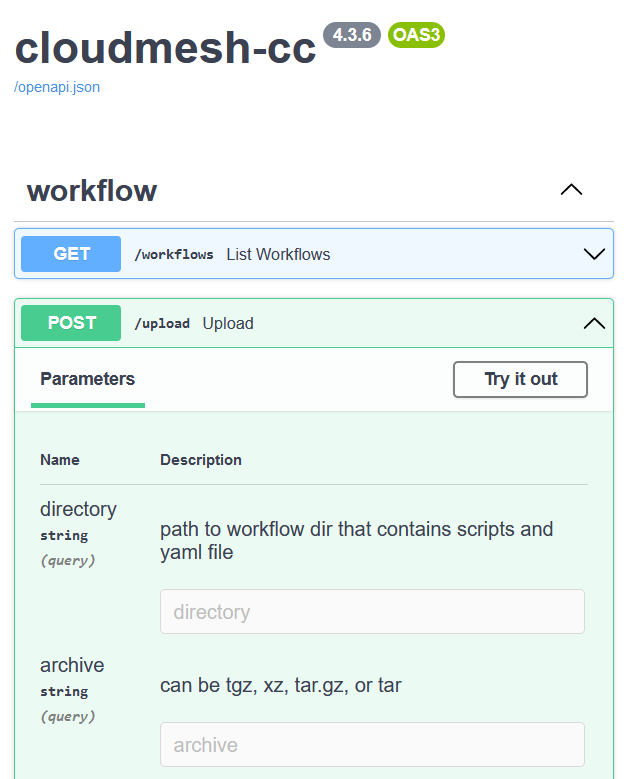
\includegraphics[width=0.52\columnwidth]{./images/upload_api.png}
}
\caption{Browser API GUI for Cloudmesh Compute Cluster.}

\label{fig:openapi}

\end{figure}


\subsection{Command Line Mode}

The command line mode is an implementation that does not use a backend
service. It runs in the terminal until the workflow is completed. All
states of the jobs are managed on the compute service on which the job
is run and the status is replicated into the client on demand. This
allows easy reporting of the status through a table and a graph
display using client-based rendering tools. The various commands to
interact with workflows on the command line are shown in
Figure~\ref{fig:code-workflow-commandline}.


\subsection{Service Mode}

The Python API has been used to implement a REST service. To easily
interact with the REST service we have also added a couple of
convenient commands one can issue from a terminal. They are listed in
Figure~\ref{fig:code-workflow-service-commandline}. It is clear from
these methods that starting, stopping, and getting the status of the
service is very easy. In contrast to the command line mode, this
service mode has an additional keyword {\em service} to interact with
the rest service.

Certainly one can also directly interact with the REST service API for
this service. For ease of use, we have exposed the interface through
an OpenAPI specification that is available to the user as shown in
Figure~\ref{fig:openapi}.

Thus, other tools such as curl or other languages supporting URL
requests can be used. A curl example to list the workflow
specifications uploaded to the service is as follows:

{\scriptsize
\begin{verbatim}
$ curl -X 'GET' 'http://127.0.0.1:8000/workflows' -H 'accept: application/json'
\end{verbatim}}
% $

As we use a REST service, we can also easily upload the workflow
through a Python-enabled REST call. We will use Python requests to
demonstrate this upload feature. To showcase the various ways to
access the service, we focus on uploading a tar file that contains the
workflow as well as the scripts or programs used in the workflow. The
tar file is called {\em workflow-example.tar}.

To also allow programming against the REST service in Python, a Python
API similar to that of the command line mode is
available. Figure~\ref{fig:code-workflow-rest-commandline} showcases
this API.

To simplify interaction with the REST service, we have created a special
{\em RESTWorkflow class} that is similar to the command module API,
but instead uses the REST interface to the service rather than direct
communication with the command client API.

The user can also simply use the requests module in Python to
interface with the API. Figure~\ref{fig:code-workflow-requests}
demonstrates how to use requests to upload a workflow by using an
archive file that contains the YAML configuration file and the
scripts.

\begin{figure}[t]

{\scriptsize
\begin{verbatim}
class RESTWorkflow
    ...
    def add_job(workflow_name, **kwargs):
        """Add a job to the workflow."""
    def delete_workflow(workflow_name, job_name=None):
        """Delete a workflow by using REST."""
    def get_workflow(workflow_name, job_name=None):
        """Retrieve a workflow by using REST."""
    def list_workflows():
        """Return a list of workflows that is found within
           the server."""
    def run_workflow( ... ):
        """Run a workflow by using REST."""
    def upload_workflow( ... ):
        """Upload a workflow by using REST."""
\end{verbatim}}

\caption{Pseudo code for the Job class with selected methods.}
\label{fig:code-workflow-rest-commandline}

\bigskip

{\scriptsize
\begin{verbatim}
  import requests
  r = requests.post(
      'http://127.0.0.1:8000/workflow?archive=workflow-example.tar')
  print(r.text)
\end{verbatim}}

\caption{Upload to the REST service with Python requests.}
\label{fig:code-workflow-requests}

\bigskip

{\scriptsize
\begin{verbatim}
  $ curl -X 'POST' 'http://127.0.0.1:8000/ 
                    workflow?archive=workflow-example.tar'
         -H 'accept: application/json' -d ''
\end{verbatim}}% $

\caption{Upload to the REST service with curl.}
\label{fig:code-workflow-curl}

\end{figure}


\subsection{Webservice GUI}

A convenient Web service is included in Cloudmesh cc. It allows the
user to manage and visualize the status of workflows through a Web
browser interface. At this time, the focus is that the interface can
be run by a single user on the local machine. This allows remote
executions of workflow nodes run completely independent from cloudmesh
cc and interaction is possible in asynchronous mode.

As the service is using also an OpenAPI 2.0 specification, the
workflow can also be uploaded implicitly through the specification
GUI. Navigate to {\scriptsize \texttt{http://127.0.0.1:8000/docs}} and
use the POST Upload method. Then click {\scriptsize \texttt{Try\ it\ out}}
and enter the location of the tar file, followed by clicking
{\scriptsize \texttt{Execute}}.

Obviously, any REST service or REST API can be used, allowing the user
to interface to it from different programming languages or frameworks.

The web server provides a more customizable, easy-to-use interface for
the Workflow class which can be started, viewed, and stopped with the
appropriate command suc as

{\scriptsize
\begin{verbatim}
  $ cms cc start
  $ cms cc view
  $ cms cc stop
\end{verbatim}}
%$

The view can also be achieved by opening the 
link \newline {\scriptsize \texttt{http://127.0.0.1:8000/}}.

The browser provides an interface to view preexisting workflows in
both a DataTable format and as a graph format. Both views will update
in a live, automatic fashion as the workflows are run, reporting
dynamic job status and progress.

For a quick and easy example of leveraging this GUI interface, click
on the Example tab in the left-hand sidebar. Then, a workflow-example
will appear underneath Workflows. Click on the workflow-example and
run the workflow by clicking the green Run button in the top-right. As
the workflow runs, the user is able to click on the Graph button to
view the graph interface (see Figure~\ref{fig:graph}) and back to the
Table button for the table interface (see Figure~\ref{fig:table}), as
desired, to view the workflow's progression.


\begin{figure}[htb]
{\centering
  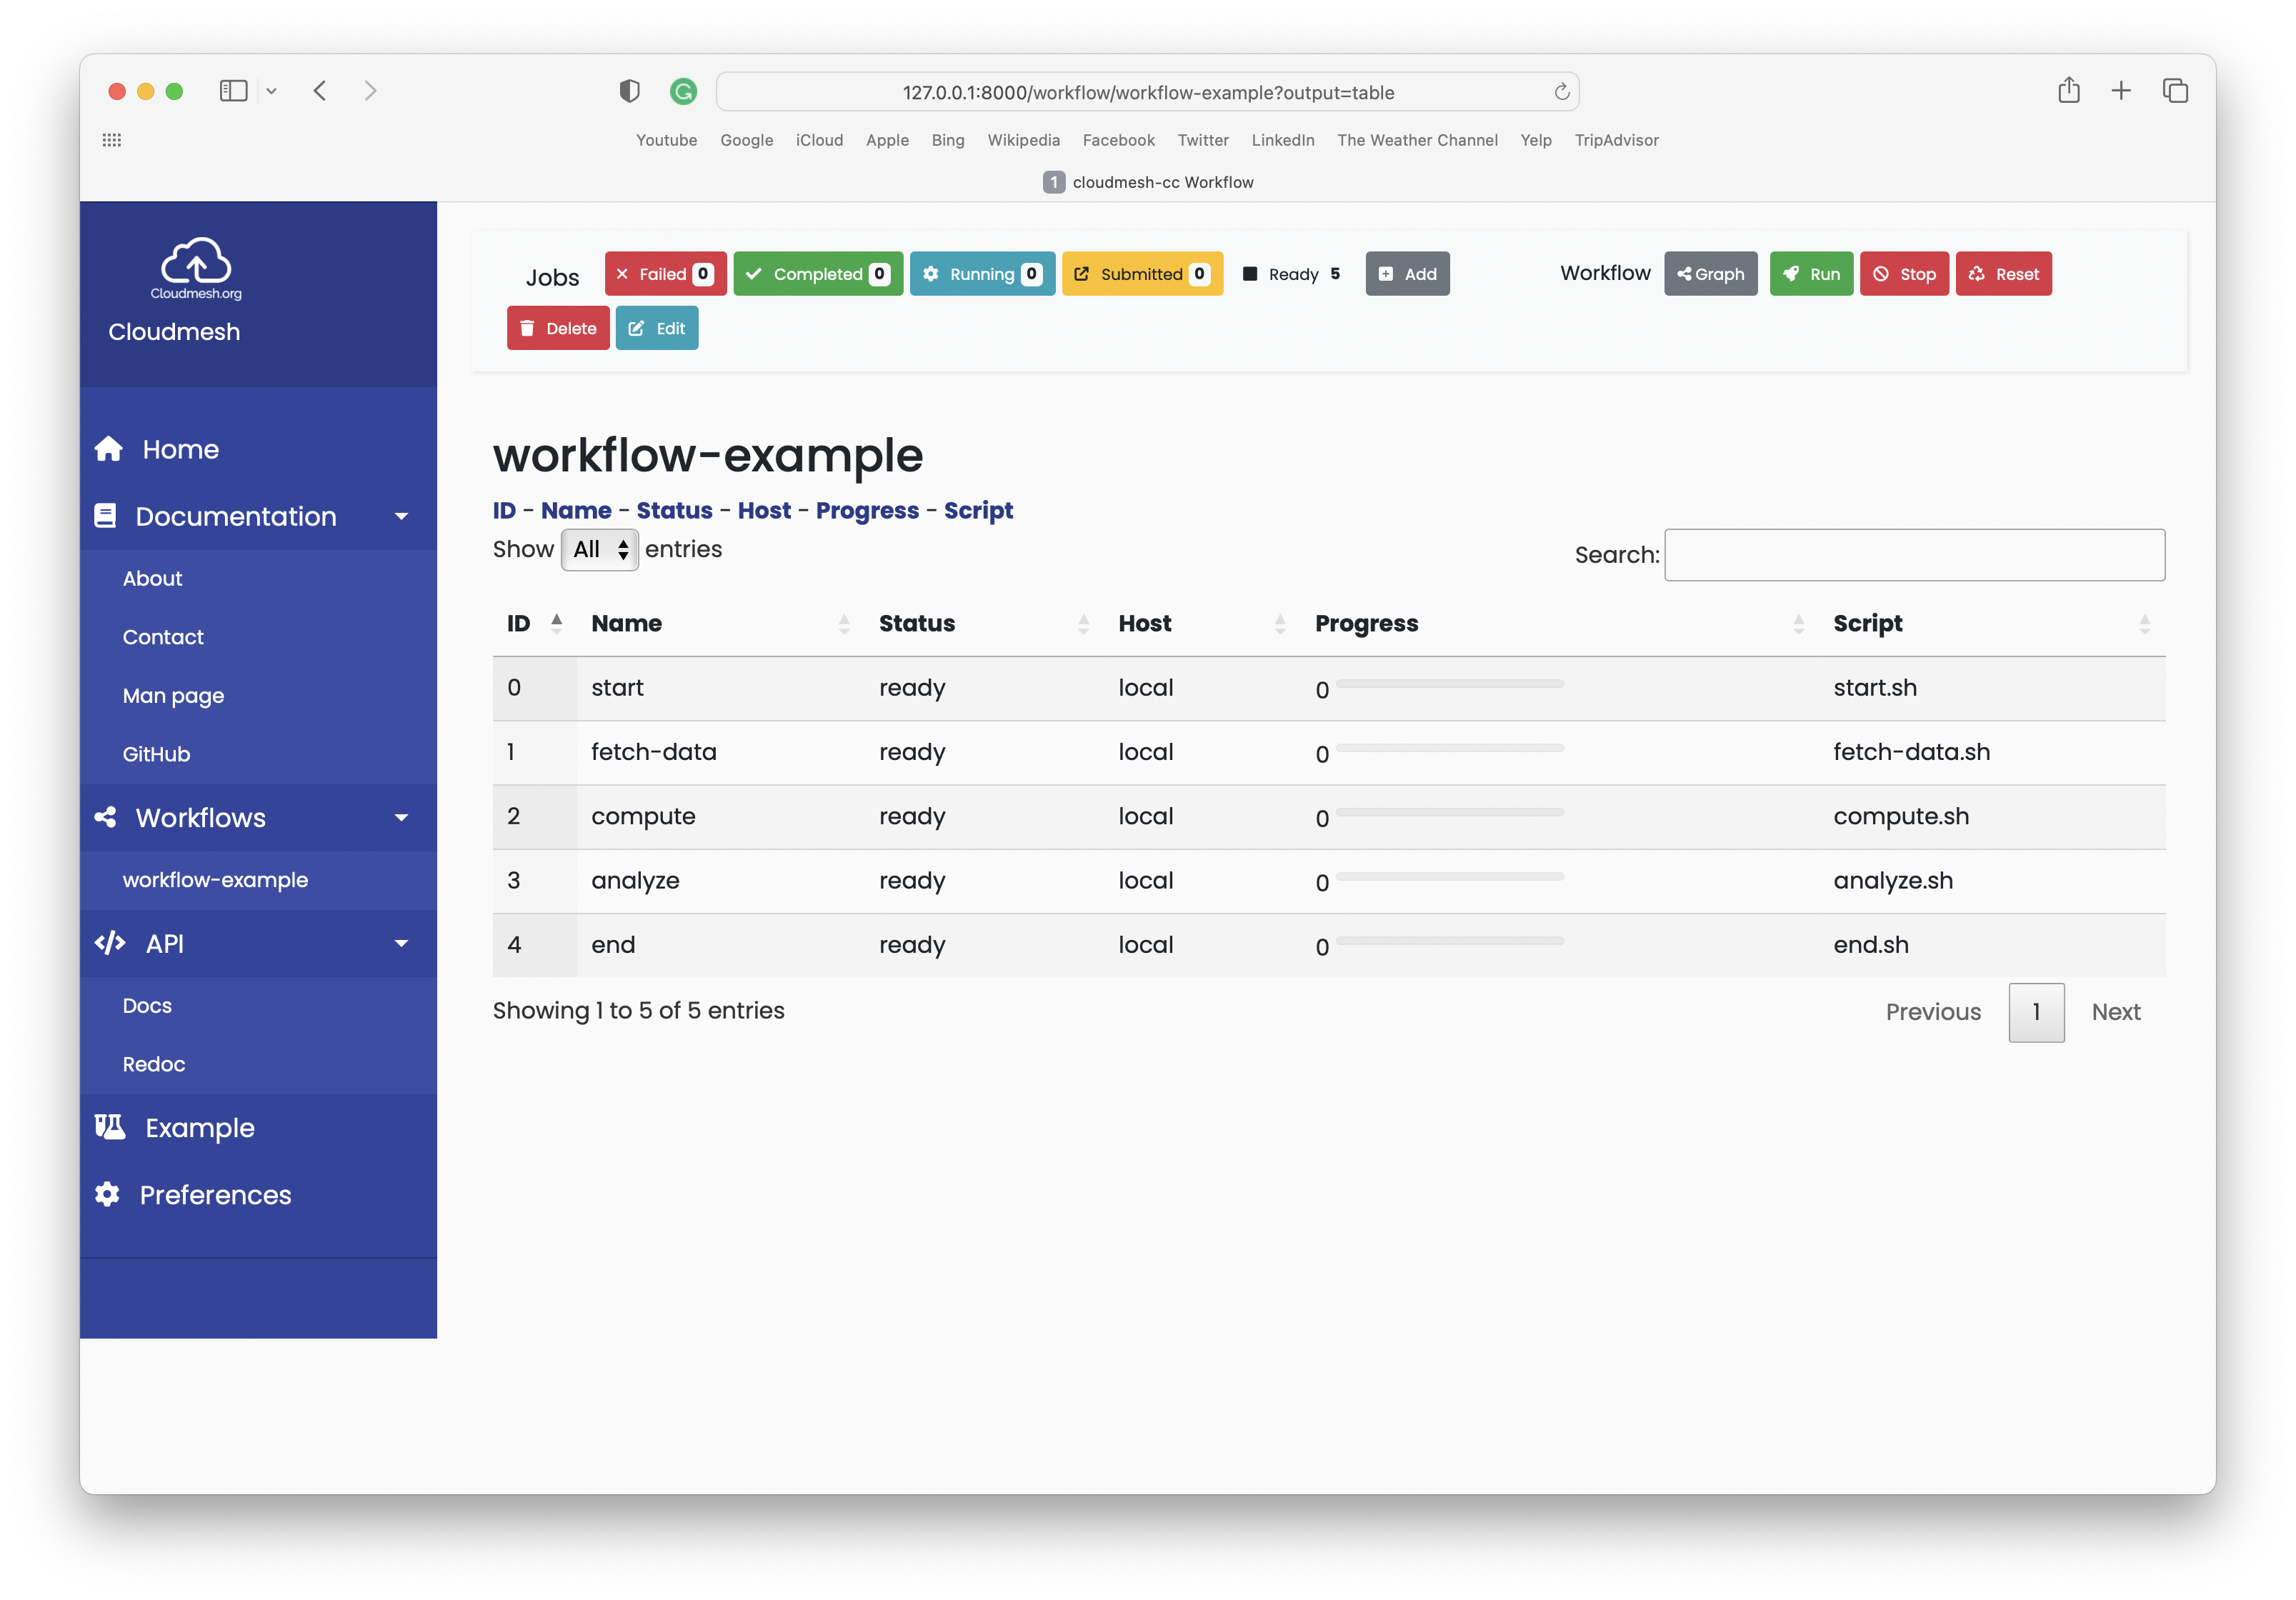
\includegraphics[width=1.0\columnwidth]{./images/service-table.png}
}
\vspace{-1.0cm}
\caption{Cloudmesh cc workflow table view.}\label{fig:table}

\bigskip
{\centering
  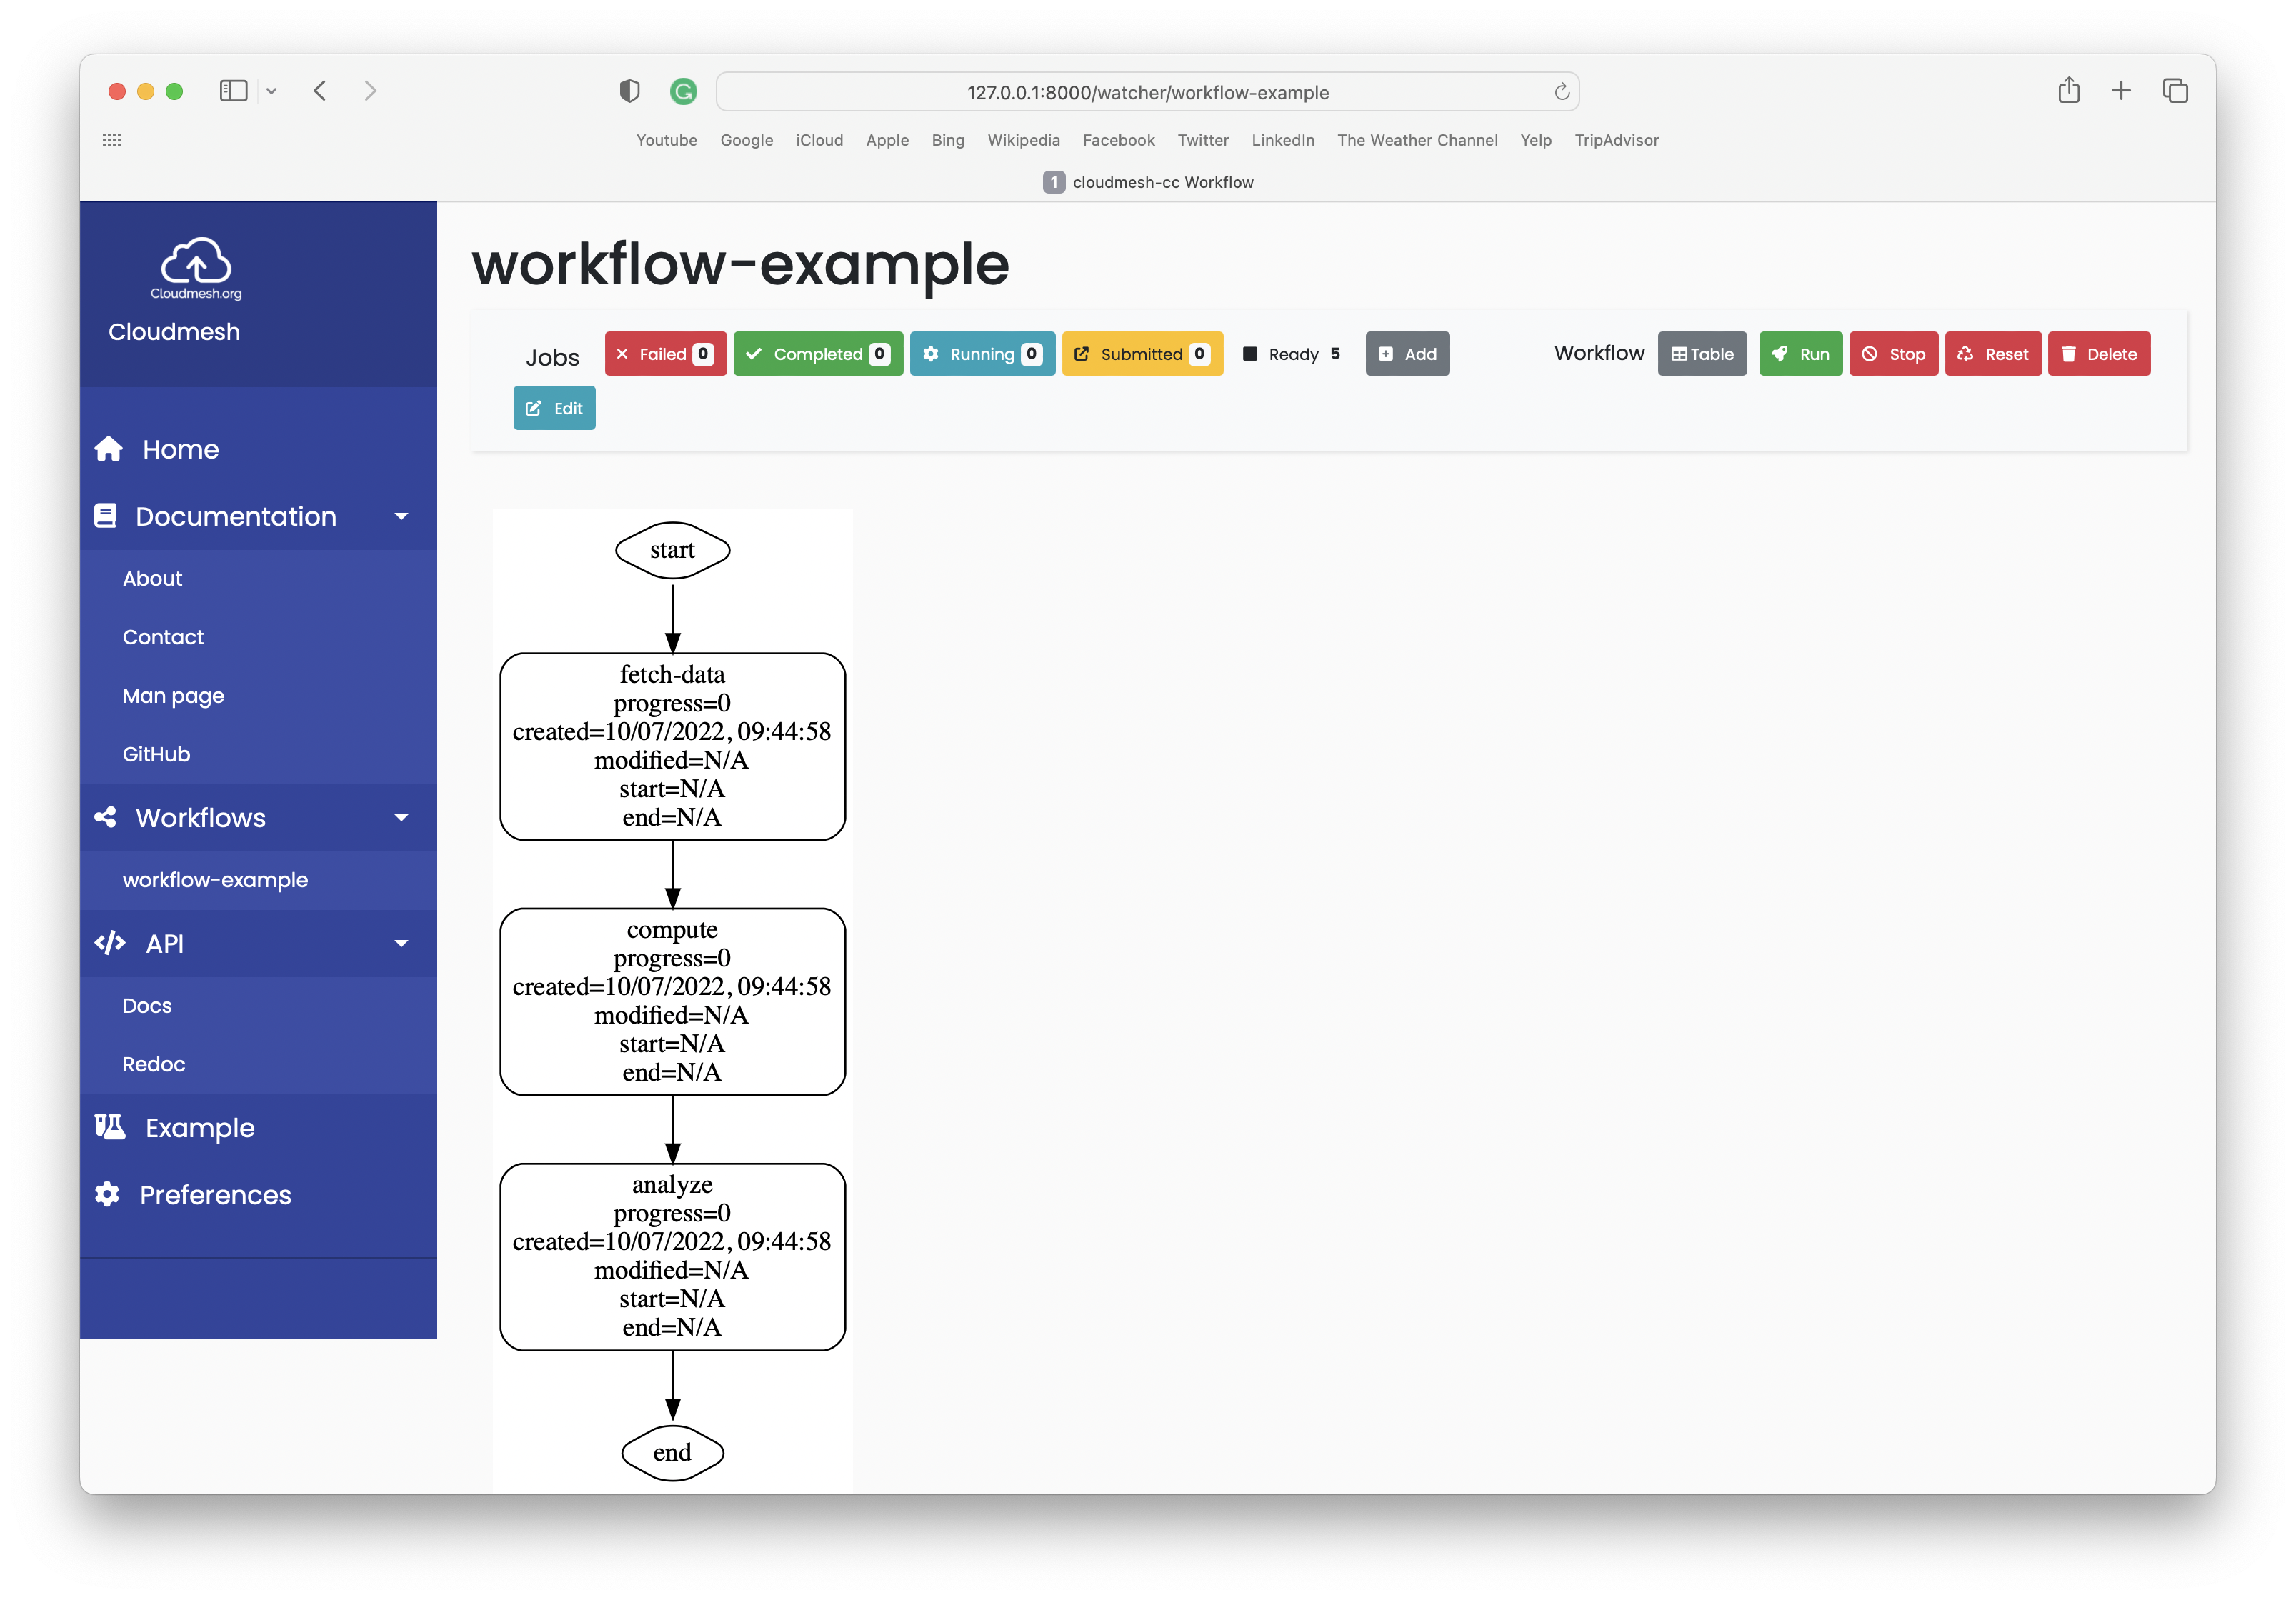
\includegraphics[width=1.0\columnwidth]{./images/service-graph.png}
 }
\vspace{-1.0cm}
 \caption{Cloudmesh cc workflow graph view.}

\label{fig:graph}
\end{figure}



\subsection{Run the workflow}\label{run-the-workflow}

The workflow can be run easily via the GUI. We added a special set of
buttons to the workflow table and graph display to simplify running of
the workflow. Certainly, the workflow can also be activated while
calling the appropriate REST call, either through Python, the OpenAPI
docs page, or, for example, a curl call.
Figures~\ref{fig:workflow-run-a}-\ref{fig:workflow-run-c}
showcase various methods to run the example workflow, which is called
{\em workflow-example}.


\begin{figure}[htb]

{\scriptsize\begin{verbatim}
  $ curl -X 'GET' 'http://127.0.0.1:8000/
                   workflow/run/workflow-example?show=True'
         -H 'accept: application/json'
\end{verbatim}}% $

\caption{Running the example workflow with curl.}
\label{fig:workflow-run-a}
\bigskip

{\scriptsize\begin{verbatim}
  from cloudmesh.cc.workflowrest import RESTWorkflow
  rest = RESTWorkflow()
  result = rest.run_workflow('workflow-example')
\end{verbatim}}

\caption{Running the example workflow with cloudmesh RESTWorkflow API.}
\label{fig:workflow-run-b}
\bigskip

{\scriptsize\begin{verbatim}
  import requests
  url = f'http://127.0.0.1:8000/workflow/run/workflow-example?show=True'
  r = requests.get(url)
  print(r)
\end{verbatim}}

\caption{Running the example workflow with requests API.}
\label{fig:workflow-run-c}

\end{figure}









% \FILE{cloudmesh.tex}

\section{Other Cloudmesh Features}

Cloudmesh comes with a sophisticated package management system, allowing to integrate packages on demand targeting varipus providers ond capabilities including a build in command shell and not just aonly a commanline tool.  Cloudmesh was first develped as a hybrid cloud API, commandline and command shell framework. It provided interfaces to AWS, Azure, Google, and OpenStack clouds for virtual machine\footnote{cloudmesh also provded support for clouds that are no longer supported such as Eucalyptsus and open cirrus. Academic clouds such as Chameloncloud were also supported.} and data file services. It is characterized be defining default templates for virtual machine management on these clouds. Hence it was possible to switch with only a view commands between clouds and stage virtual machines on them such as demonstarted in Figure~\ref{fig:cms}.

\begin{figure}[htb]

\begin{minted}[breaklines]{bash}
$ cms vm start --cloud aws
$ cms vm start --cloud azure
\end{minted}

  \caption{Simple VM managegment for hybrid clouds}
\label{fig:cms}.
\end{figure}  

In addition we have also developed a pacage called GAS that addresses the creation of analytics REST services from python functios. This package was developed to address the problem that integrating deployment frameworks in the age of cloud computing is often out of reach for domain experts.  GAS is a simple frameworks allowing even non-experts to deploy and host services in the cloud. To avoid vendor lock-in it supports multiple vendors through the use of cloudmesh vm management \cite{las21-gas}.


\FILE{cloudmesh.tex}

\section{Other Cloudmesh Features}

Cloudmesh comes with a sophisticated package management system,
allowing the integration of packages on demand targeting various providers
and capabilities including a built-in command shell (not just only
a command line tool). Cloudmesh was first developed as a hybrid cloud
API, command line and command shell framework. It provided interfaces
to AWS, Azure, Google, and OpenStack clouds for virtual
machine\footnote{cloudmesh also provided support for clouds that are no
longer supported such as Eucalyptus and Open Cirrus. Academic clouds
such as Chameleon Cloud were also supported.} and data file services. It
is characterized by defining default templates for virtual machine
management on these clouds. Hence, it was possible to switch between clouds
with only a few commands and stage virtual machines on them, such
as with the commands demonstrated in Figure~\ref{fig:cms}.

\begin{figure}[htb]

{\scriptsize\begin{verbatim}
  $ cms vm start --cloud aws
  $ cms vm start --cloud azure
\end{verbatim}}

\caption{Simple VM management for hybrid clouds}
\label{fig:cms}.
\end{figure}  

In addition, we have developed a package called GAS that addresses
the creation of analytics REST services from Python functions. This
package was developed to address the problem that integrating
deployment frameworks in the age of cloud computing is often out of
reach for domain experts. GAS is a simple framework allowing even
non-experts to deploy and host services in the cloud. To avoid vendor
lock-in, it supports multiple vendors through the use of cloudmesh vm
management~\cite{las21-gas}.


% \FILE{applications.tex}

\section{Workflow Applications}

We have applied the workflow system on a number of appliactions. All workflows for these applications are avaialable in our GitHub and can be adapted easily.
This includes the Cloudmask and MNIST application workflows which we describe next in more details.



\FILE{applications.tex}

\section{Workflow Applications}

We have applied the workflow system on a number of applications. All
workflows for these applications are available in our GitHub and can
be adapted easily. This includes the Cloudmask and MNIST application
workflows which we describe next in more details.




% \section{Cloudmask Workflow}\label{cloudmask-workflow}

Cloudmesh cc comes with an example workflow that runs Cloudmask, which
is a program that develops a model to classify sections of satellite
images. Information regarding Cloudmask can be found at
\url{https://github.com/laszewsk/mlcommons/tree/main/benchmarks/cloudmask\#readme}

\subsection{Running the Cloudmask Workflow on
Rivanna}\label{running-the-cloudmask-workflow-on-rivanna}

To execute the workflow on UVA's HPC supercomputer, Rivanna, first
ensure that your UVA Computing ID is set with the following command,
replacing the X's with your ID:

\begin{verbatim}
me@mycomputer $ cms set username=XXXXXX
\end{verbatim}

Then, connect to the UVA Anywhere VPN and then download the satellite
data into your
\href{https://www.rc.virginia.edu/userinfo/storage/non-sensitive-data/\#scratch}{scratch}
directory on Rivanna:

\begin{verbatim}
me@mycomputer $ cms vpn connect
me@mycomputer $ ssh rivanna
rivanna $ cd /scratch/$USER
rivanna $ git clone https://github.com/laszewsk\
/mlcommons.git
rivanna $ cd mlcommons/benchmarks/cloudmask\
/target/rivanna
rivanna $ make data
# downloading the data will take a while.
rivanna $ exit
\end{verbatim}

Next, clone the \texttt{mlcommons} repository on your local machine and
run the workflow:

\begin{verbatim}
me@mycomputer $ cd ~/cm
me@mycomputer $ git clone https://github.com\
/laszewsk/mlcommons.git
me@mycomputer $ cd mlcommons
me@mycomputer $ pytest -v -x --capture=no \ 
benchmarks/cloudmask/target/rivanna/run_cloudmask\
_workflow.py
\end{verbatim}

The workflow iterates through the five GPUs available on Rivanna---
A100, V100, P100, RTX2080, and K80--- and runs the program three times
on each GPU. Each run trains the model with 10, 30, and 50 epochs for
benchmarking.

Upon completing a run, the logs and benchmarks of the program can be
found in the target folder:

\begin{verbatim}
me@mycomputer $ ssh rivanna
rivanna $ cd /scratch/$USER/mlcommons\
/benchmarks/cloudmask/target
\end{verbatim}

Additionally, the generated \texttt{.h5} model file can be found in the
home directory:

\begin{verbatim}
 rivanna $ cd ~/sciml_bench/outputs/slstr_cloud/
 \end{verbatim}

The program may take a while to run if the resources on Rivanna are
being used by other jobs.


\FILE{Cloudmask.tex}

\subsection{MLCommons Cloudmask Workflow}
\label{cloudmask-workflow}

Cloudmask is a program that develops a model to classify sections of
satellite images as either containing clouds or clear sky by using
machine learning. This is beneficial for temperature measurement and
meteorology. Information regarding Cloudmask can be found on its
GitHub page~\cite{www-cloudmask}. One of our goals is to run
Cloudmask for benchmarking. As benchmarking Cloudmask requires
several phases and scripts, including a mixture of shell scripts and
Python scripts, leveraging Cloudmesh-cc provides a much easier runtime
instead of manually issuing many commands at a terminal. We have
created a sample workflow the runs a coordinated workflow across a
number of hybrid resources. This includes an HPC computer at the
University of Virginia called Rivanna, as well as two desktop
computers. This workflow can easily be adapted to include other
machines. In this particular workflow, we execute the benchmarks on a
number of different CUDA cards (see Figure~\ref{fig:cloudmaskwf}. For
Rivanna, the code also utilizes our cloudmesh-vpn component that
provides the ability to connect to the UVA VPN from Python, then
fetches the data and executes the various benchmarks once the data is
available.

\begin{figure*}[htb]
\centering
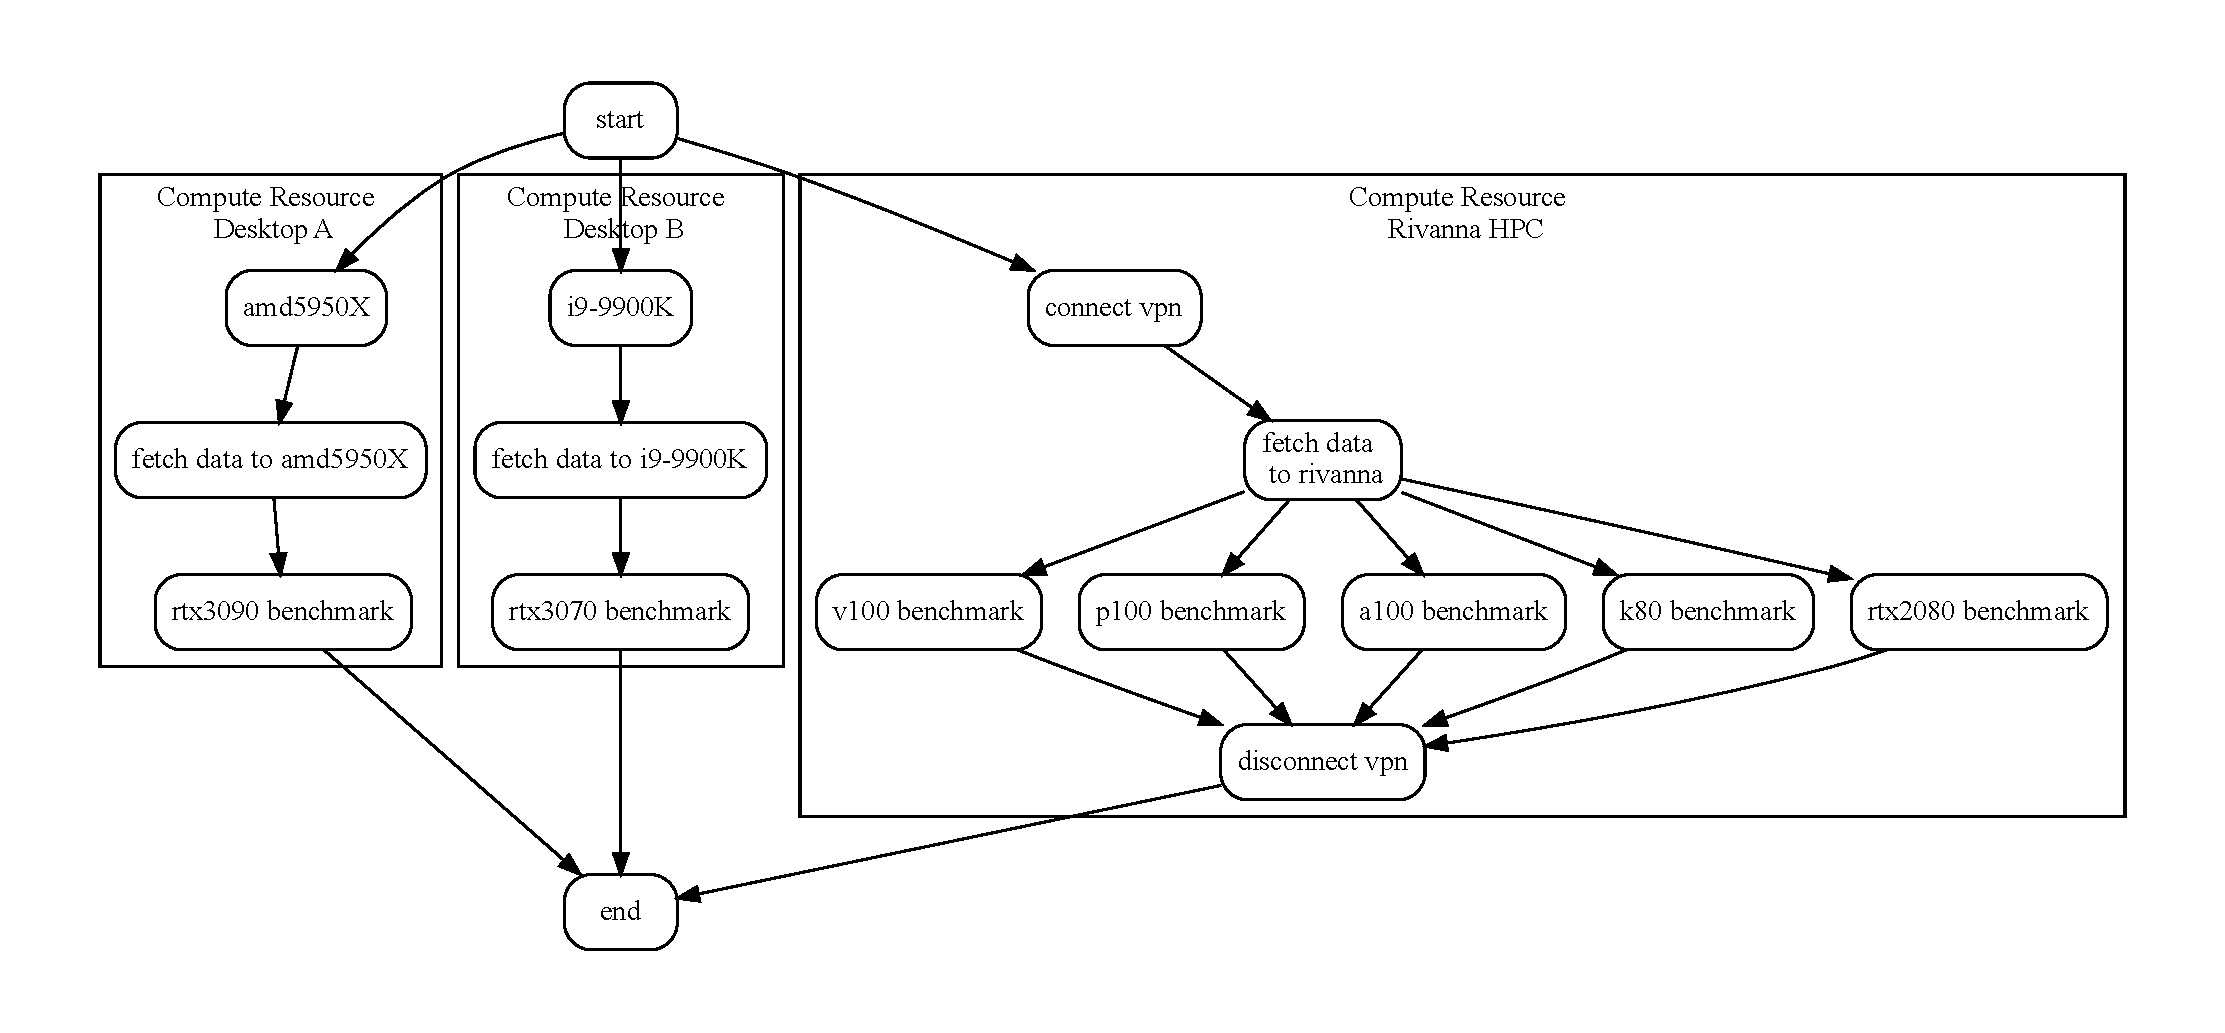
\includegraphics[width=0.75\textwidth]{./images/cloudmask-wf.pdf}
%\vspace{-1cm}
\caption{Workflow for Cloudmask}\label{fig:cloudmaskwf}
\end{figure*}

The workflow will take approximately 24 hours to run if resources are
available. The workflow iterates through the five GPUs available on
Rivanna, including V100, P100, A100, K80, and RTX2080, and runs the
program three times on each GPU. Each run trains the model with 10,
30, and 50 epochs for benchmarking. Upon completing a run, the logs
and benchmarks are written into a results folder. In the appendix, we
showcase how to run a portion of this workflow while utilizing
only Rivanna (see Appendix~\ref{sec:running-cloudmask}).



%\section{MNIST Workflow}\label{mnist-workflow}

For this example we use UVA's Rivanna machine. Please adopt it to your
HPC machine.

We can test Rivanna's GPUs and benchmark their runtimes for running
several MNIST Python programs. These programs include machine learning
processing, convolutional neural network, long short-term memory,
recurrent neural network, and others. The programs can be found at
\url{https://github.com/cybertraining-dsc/reu2022/tree/main/code/deeplearning/mnist}

To run the MNIST remote workflow on Rivanna, first ensure that your UVA
computing ID is set with the following command:

\begin{verbatim}
cms set username=XXXXXX
\end{verbatim}

where the X's are substituted with your computing ID.

Then, issue commands:

\begin{verbatim}
cd ~/cm/cloudmesh-cc
pytest -v -x --capture=no examples/example_run_mnist_workflow_exec.py
\end{verbatim}

This program uses SLURM and a shell script to iterate through the
available GPUs on Rivanna, which are V100, A100, K80, P100, and RTX2080.

On a successful run, the output will be similar to the following:

\begin{verbatim}
+---------+----------+---------+---------+---------------------+
| Name    | Status   |    Time |     Sum | Start               |
|---------+----------+---------+---------+---------------------+
| v100    | ok       | 138.087 | 138.087 | 2022-09-29 18:15:45 |
| a100    | ok       | 106.046 | 106.046 | 2022-09-29 18:18:05 |
| k80     | ok       | 171.057 | 171.057 | 2022-09-29 18:19:52 |
| p100    | ok       | 202.055 | 202.055 | 2022-09-29 18:22:44 |
| rtx2080 | ok       | 138.048 | 138.048 | 2022-09-29 18:26:07 |
+---------+----------+---------+---------+---------------------+
\end{verbatim}


\FILE{mnist.tex}

\subsection{MNIST Workflow}\label{mnist-workflow}

MNIST is a well-known program to detect handwritten digits. It
provides value for our work because it is well understood and is used
in many educational efforts. Also, we created a workflow that
integrates the UVA Rivanna HPC (the workflow can easily be adapted to other
machines). The nice feature about this application is that it can be
configured to run very quickly while still using various GPUs and
benchmark their runtimes for running several MNIST Python
programs. These programs include machine learning processing,
convolutional neural network, long short-term memory, recurrent neural
network, and others. The programs can be found on
GitHub~\cite{www-mnist-programs}.

As for the workflow, we adapted it not only to run one algorithm but
multiple in an iteration across the GPUs (similar to
\ref{fig:cloudmaskwf}).

On a successful run, the output will be receiving runtimes similar to:

\begin{table}[!ht]
\caption{MNIST Performance as obtained by cloudmesh-cc on various graphics cards using workflow scheduling}
    \centering
    \begin{tabular}{lr}
    \hline
        Name & Time \\ \hline
        a100 & 106.046 \\ 
        v100 & 138.087 \\ 
        rtx2080 & 138.048 \\
        k80 & 171.057 \\ 
        p100 & 202.055 \\
    \end{tabular}
    \label{table:mnist-times}
  \end{table}
  


% \FILE{conclusion.tex}

\section{Conclusion}

TBD

\FILE{conclusion.tex}

\section{Conclusion}

We have designed and implemented a Hybrid Reusable Computational
Analytics Workflow Management with the help of the cloudmesh component
framework. The component added focuses on the management of workflows
for computational analytics tasks and jobs. The tasks can be executed
on remote resources via ssh and even access queuing systems such as
Slurm. In addition, we can integrate the current computer on which the
workflow is running. This can include operating systems such as Linux,
macOS, Windows, and even Windows Subsystem for Linux. Through
cloudmesh, access to a command line and a command shell is provided. A
simple API and a REST interface are provided. The framework also has
an elementary Web browser interface that allows visualizing the
execution of the workflow. It is important to know that the workflow
can be started on remote resources and is running completely
independently from the client tool once a task is started. This allows
a ``stateless'' model that can synchronize with the remotely started
jobs on demand. Hence, the framework is self-recovering in case of
network interruptions or power failure. Due to our experiences with
real (and many) infrastructure failures at the authors' locations, the
availability of such a workflow-guided system was
beneficial. Furthermore, the developed code is rather small and, in
contrast to other systems, is less complex. Hence, it is suitable for
educational aspects as it is used for master's and undergraduate level
research projects. The project has also been practically utilized
while generating benchmarks for the MLCommons Science Working Group
showcasing real-world applicability beyond a student research project.


% \FILE{acknowledgements.tex}

%\begin{ack}

\section*{Acknowledgements}

Continued work was in part funded by the NSF CyberTraining: CIC:
CyberTraining for Students and Technologies from Generation Z with the
award numbers 1829704 and 2200409 and NIST 60NANB21D151T. We like to
thank the students that participated in the REU for their help and
evaluation in a pre-alpha version of the code. We are excited that
this effort contributed significantly to their increased understanding
of Python and how to develop in a team using the Python ecosystem.

%\end{ack}


\FILE{acknowledgements.tex}

%\begin{ack}

\section*{Acknowledgements}

Continued work was in part funded by the NSF CyberTraining: CIC:
CyberTraining for Students and Technologies from Generation Z with the
award numbers 1829704 and 2200409 and NIST 60NANB21D151T. We would like to
thank the students that participated in the REU for their help and
evaluation in a pre-alpha version of the code. We are excited that
this effort contributed significantly to their increased understanding
of Python and how to develop in a team using the Python ecosystem.

%\end{ack}


\bibliographystyle{ACM-Reference-Format}
\bibliography{vonLaszewski-cloudmesh-cc}


\appendix

\section{Appendix}

% \FILE{installation.tex}

\section{Installation}\label{installation}

To leverage cloudmesh-cc, use the cloudmesh-installer to install the
Cloudmesh suite of repositories. Optionally, to utilize the graph
visualization you must install also {\em graphviz} must be
installed. On Windows, Git Bash is required, in addition.  The overall
installation is very simple and is supported on a variety of operating
systems.  We leverage the cloudmesh-installer to locally install the
cloudmesh suite of repositories by executing the following commands:

\begin{minted}[breaklines]{bash}
$ mkdir ~/cm
$ cd ~/cm
$ pip install cloudmesh-installer -U
$ cloudmesh-installer get cc
\end{minted}

To install graphviz you can use the following commands on the appropriate operating system:

\begin{description}

\item[Windows.]
Git Bash and Graphviz must be installed. The user can use Chocolatey to run
as an administrator for convenience:

\begin{minted}[breaklines]{bash}
$ choco install git.install --params "/GitAndUnixToolsOnPath /Editor:Nano /PseudoConsoleSupport /NoAutoCrlf" -y
$ choco install graphviz -y
\end{minted}

\item[macOS.] Graphviz must be installed. The user can use Homebrew for convenience:

\begin{minted}[breaklines]{bash}
$ brew install graphviz
\end{minted}

\item[Linux.] Graphviz must be installed. The user can use apt for convenience:

\begin{minted}[breaklines]{bash}
$ sudo apt install graphviz -y
\end{minted}

\end{description}

To test the workflow program, prepare a cm directory in your home
directory by executing the following commands:

\begin{minted}[breaklines]{bash}
$ cd ~/cm/cloudmesh-cc
$ pytest -v -x --capture=no tests
\end{minted}

A variety of separate tests are available that test individual capabilities. 


\FILE{installation.tex}

\subsection{Installation}\label{installation}

To leverage cloudmesh-cc, use the cloudmesh-installer to install the
Cloudmesh suite of repositories. Optionally, to utilize the graph
visualization you must install also {\em graphviz} must be
installed. On Windows, Git Bash is required, in addition. The overall
installation is very simple and is supported on a variety of operating
systems. We leverage the cloudmesh-installer to locally install the
cloudmesh suite of repositories by executing the following commands:

{\scriptsize\begin{verbatim}
  $ mkdir ~/cm
  $ cd ~/cm
  $ pip install cloudmesh-installer -U
  $ cloudmesh-installer get cc
\end{verbatim}}

To install graphviz you can use the following commands on the
appropriate operating system:

\begin{description}

\item[Windows.]  Git Bash and Graphviz must be installed. The user
can use an instance of Chocolatey that is run as an administrator for
convenience:

{\scriptsize\begin{verbatim}
  $ choco install git.install
          --params "/GitAndUnixToolsOnPath
                    /Editor:Nano
                    /PseudoConsoleSupport
                    /NoAutoCrlf" -y
  $ choco install graphviz -y
\end{verbatim}}

\item[macOS.] Graphviz must be installed. The user can use Homebrew
for convenience:

{\scriptsize\begin{verbatim}
  $ brew install graphviz
\end{verbatim}}

\item[Linux.] Graphviz must be installed. The user can use apt for
convenience:

{\scriptsize\begin{verbatim}
  $ sudo apt install graphviz -y
\end{verbatim}}

\end{description}

To test the workflow program, prepare a {\scriptsize \verb|cm|}
directory in your home directory by executing the following commands:

{\scriptsize\begin{verbatim}
  $ cd ~/cm/cloudmesh-cc
  $ pytest -v -x --capture=no tests
\end{verbatim}}

A variety of separate tests are available that test individual
capabilities.


% \FILE{cloudmask-appendix.tex}

\subsection{Running Cloudmask Workflow}\label{sec:running-cloudmask}

To run the Cloudmask workflow, run the following commands:

\begin{minted}[breaklines]{bash}
$ cd ~/cm
$ git clone https://github.com/laszewsk/mlcommons.git
$ cd mlcommons
$ pytest -v -x --capture=no benchmarks/cloudmask/target/rivanna/run_cloudmask_workflow.py
\end{minted}


\FILE{cloudmask-appendix.tex}

\subsection{Running Cloudmask Workflow}\label{sec:running-cloudmask}

To run the Cloudmask workflow, run the following commands:

{\scriptsize\begin{verbatim}
  $ cd ~/cm
  $ git clone https://github.com/laszewsk/mlcommons.git
  $ cd mlcommons
  $ pytest -v -x --capture=no
           benchmarks/cloudmask/target/rivanna/run_cloudmask_workflow.py
\end{verbatim}}


% \section{Contributing}\label{contributing}

\subsection{GitHub}\label{github}

The code is maintained on GitHub

\begin{itemize}
\tightlist
\item
  \href{https://github.com/cloudmesh/cloudmesh-cc}{Code}
\item
  \href{https://github.com/cloudmesh/cloudmesh-cc/issues}{Issues}
\item
  \href{https://github.com/cloudmesh/cloudmesh-cc/pulls}{Pull Requests}
\item
  \href{https://github.com/cloudmesh/cloudmesh-cc/actions}{Actions}
\item
  \href{https://github.com/cloudmesh/cloudmesh-cc/pulse}{Insights}
\end{itemize}

The code was developed by Gregor von Laszewski and J.P. Fleischer. Other
contributors to a pre alpha version are listed at

\begin{itemize}
\tightlist
\item
  \href{https://github.com/cloudmesh/cloudmesh-cc/graphs/contributors}{Contributors}
\end{itemize}

\subsection{Management}\label{management}

All contributions will be done under the apache license. The code will
be managed in open-source. Pull requests need to be made in the
repository. The main branch is the release branch. Contributions will
first be done in other branches, and once we agree that they need to be
integrated into the code, they will be merged into main. All new code
must have sufficient pytests. The pytests may need to be documented in
case special authentication is required.

We follow a
\href{https://docs.github.com/en/get-started/quickstart/github-flow}{typical
GitHub workflow} of:

\begin{itemize}
\tightlist
\item
  create a personal fork of this repo
\item
  create a branch
\item
  open a pull request
\item
  fix findings of various linters and checks
\item
  work through code review
\end{itemize}

For each pull request, the documentation is built and deployed to make
it easier to review the changes in the pull request.

\hypertarget{tests}{%
\subsection{Tests}\label{tests}}

Before creating a pull request it is important that the tests in the
test directory pass.

The tests are organized as follows:

\begin{itemize}
\tightlist
\item
  \texttt{pytest\ tests/test\_0??\_*} will run locally and only use
  ascii output
\item
  \texttt{pytest\ tests/test\_1??\_*} will run locally but also present
  graphs
\end{itemize}

in future we will likely change this and allow a test variable
\texttt{cms\ set\ test\_with\_graph=False/True} and if it is not
existent it is False. In case it is false the graohs will not be
displayed. but the test will be run. This change will also allow tests
with 1?? to be run on github workflows

\begin{itemize}
\tightlist
\item
  \texttt{pytest\ tests/test\_5??\_*} will run on remote machines and
  require at this time rivanna from UVA
\end{itemize}

in future this test will be modified so we can specify the remote user
and remote host \texttt{cms\ set\ test\_remote\_user=TBD}
\texttt{cms\ set\ test\_remote\_host=TBD}. If they do not exist they
will use the defualts from ssh config rivanna. verify if logic is ok.

\begin{itemize}
\tightlist
\item
  \texttt{pytest\ tests/test\_6??\_*} will test the rest service
\item
  \texttt{pytest\ tests/test\_9??\_*} will cleanup the tests
\end{itemize}


\FILE{contributing.tex}

\subsection{Contributing}\label{contributing}

All contributions are done under the Apache License. The code is
maintained as an open-source project on GitHub while using the typical
GitHub code management tools such as:

\begin{itemize}
\item
  \href{https://github.com/cloudmesh/cloudmesh-cc}{Code Repository}
\item
  \href{https://github.com/cloudmesh/cloudmesh-cc/issues}{Issue Management}
\item
  \href{https://github.com/cloudmesh/cloudmesh-cc/pulls}{Pull Request Management}
\item
  \href{https://github.com/cloudmesh/cloudmesh-cc/actions}{Automatic verification with GitHub Actions}
\end{itemize}

The main branch is the release branch and is supposed to be functional
at all times. Hence, contributions are first done in other branches,
and once agreeing that they need to be integrated into the code, they
are merged into main. All new code must be documented and have
sufficient automated tests. Before creating a pull request, it is
important that the tests within the test directory are passing. The
repository already contains several pytests that can be leveraged to
conduct routine testing of the code, including its SSH remote
functionality, REST capability, and Python interface, among others.



\end{document}
\endinput
%%
%% End of file `sample-sigplan.tex'.
